\documentclass{article}
\usepackage{polski}
\usepackage{babel}[polish]
\usepackage[utf8]{inputenc}
\usepackage{makecell}
\usepackage{hyperref}
\usepackage{xcolor}
\setcounter{tocdepth}{3}
\textheight 23.2 cm
\textwidth 6.0 in
\hoffset = -0.7 in % -0.5 in
\voffset = -2.4 cm
\usepackage{natbib}
\usepackage{graphicx}
\begin{document}

\title{
\includegraphics[width=\textwidth]{MINI logo long.png}\\
        System rezerwacji pokoi hotelowych
        \noindent\rule{\textwidth}{1pt}\\
        IO PROJEKT - Finalna Specyfikacja}
\author{Artur Michalski, Ignacy Sujecki, Mateusz Tabor,\\Dawid Maksymowski, Damian Wyszołmirski}
\maketitle

\tableofcontents
\addtocontents{toc}{\protect\hypertarget{toc}{}}
\newpage
\section{Wprowadzenie}

Celem projektu jest stworzenie systemu do rezerwacji pokoi w hotelach. Aplikacja pozwala obsłudze hotelu na udostępnienie oferty w systemie, a użytkownikowi na zarezerwowanie pokoju z oferty w określonym oknie czasowym. Obsługa hotelu dzieli się na pracowników z różnym poziomem dostępu do zasobów aplikacji. Manager hotelu pełni rolę administratora modułu hotelowego. Serwer aplikacji przetrzymuje kopie wszystkich ofert, więc po złożeniu rezerwacji i sprawdzeniu kieruje prośbę do systemu hotelowego, gdzie hotel jeszcze raz potwierdza dostępność.
%i oczekuje na płatność. Po otrzymaniu zapłaty system potwierdza rezerwację.\\
\subsection{Glosariusz}
Poniżej znajdują się definicje kluczowych elementów naszego systemu. Warto wśród nich zwrócić uwagę na rozróżnienie Pokoju oraz Oferty. Podział taki został zastosowany, aby nie powielać tych samych informacji wśród różnych pokoi, będących w istocie takimi samymi z punktu widzenia Klienta.

\begin{itemize}
    \item \textbf{Pokój}\\
    Reprezentuje fizyczny pokój obecny w hotelu, w którym się znajduje. Jest konkretnym reprezen\-tantem Oferty (patrz: następny punkt). Dane dotyczące pokoi są przechowywane w bazie danych Hotelu. Najwygodniej, gdy jego ID jest tożsame z fizycznym numerem pokoju, jednak – jako, że informacje o tych obiektach są przechowywane w lokalnej bazie hotelu – identyfikacja leży całkowicie w gestii zarządcy tej bazy.
    \item \textbf{Oferta}\\
    Reprezentuje pokoje o takich samych parametrach, które są nierozróżnialne z punktu widzenia Klienta rezerwującego pokój. Oferta ma określoną liczbę gości (dorosłych oraz dzieci), posiada opis i (opcjonalnie) zdjęcia.
    Ponieważ oferta jest tworzona lokalnie w module hotelowym, jest rozróżnialna przez ID hotelu, w którym się znajduje oraz jej lokalne ID.
    \item \textbf{Rezerwacja}\\
    Reprezentuje wynajem pokoju przez klienta w określonym odcinku czasowym. Klient dokonuje rezerwacji pokoju poprzez wybranie Oferty. To, który Pokój zostanie przypisany do Rezerwacji jest decyzją hotelu.
    ID rezerwacji jest przypisywane przez hotel i unikatowe w obrębie modułu hotelowego.
    \item \textbf{Opinia}\\
    Po pobycie w danym hotelu w ciągu 30 dni klient ma możliwość wystawienia opinii, czyli krótkiego opisu swoich przeżyć w hotelu wraz z oceną w skali od 1 do 10. Opinia jest przetrzy\-mywana przez serwer i dołączana do wysyłanych ofert hotelu którego dotyczy.
    ID opinii jest przypisywane przez serwer więc jest unikalne w całym systemie.
    \item \textbf{Klient}\\
    Użytkownik Aplikacji klienckiej, który może w systemie się zarejestrować oraz zalogować. Tylko za pośrednictwem konta Klienckiego możliwe jest przeglądanie Ofert, Hoteli oraz złożenie rezerwacji.
    ID klienta jest przypisywane przez serwer więc jest unikalne w całym systemie.
    \item \textbf{Hotel}\\
    Reprezentuje fizyczną jednostkę hotelu rzeczywistego świata. Dodawanie Ofert i reklamowanie się do potencjalnych klientów za pośrednic\-twem Systemu jest możliwe wyłącznie za pośrednictwem takiego konta.
    \item \textbf{Pracownik}\\
    Reprezentuje fizyczną osobę pracującą w hotelu. Posiada uprawnienia i w zależności od nich może edytować i pobierać dane z systemu hotelowego, które mogą usprawniać jego pracę.
\end{itemize}

\newpage
\section{Podział na moduły}
System składa się z 3 modułów niezależnych od siebie. Mogą one (choć nie muszą) być uruchomione i działać na oddzielnych maszynach.
Moduły te to:
\begin{itemize}
  \item Aplikacja Kliencka
  \item System Hotelowy
  \item Moduł Serwerowy
\end{itemize}

\subsection{Aplikacja Kliencka}
Ten moduł wyposażony jest w interfejs graficzny pozwalający na wyświetlanie ofert wraz ze zdjęciami i list dostępnych ofert do wyboru oraz w wyszukiwarkę. Pozwala również klientowi zarezerwować pokój(przez wybór oferty i kliknięcie "rezerwuj"), anulować rezerwacje, a także zostawiać opinię dotyczącą odbytego pobytu.
Moduł ten porozumiewa się tylko z modułem serwerowym.
W systemie jest dowolna liczba instancji modułów Aplikacji Klienckiej.

\subsection{Moduł Hotelowy}
Moduł zwiera interfejs graficzny pozwalający na wyświetlanie informacji oraz modyfikowanie i dostęp do danych hotelowych związanych z dostępnymi ofertami jak i rezerwacjami, pokojami hotelowymi czy użytkownikami systemu hotelowego (obsługa hotelowa). Moduł hotelowy zawiera system uprawnień użytkowników jak i konto administracyjne służące do zarządzania systemem hotelowym. Moduł ten komunikuje się tylko z serwerem.
W systemie może być dowolna liczba instancji modułów hotelowych.

\subsection{Moduł Serwerowy}
System ten posiada interfejs konsolowy. Pośredniczy on w komunikacji pomiędzy hotelami i klientami, oraz przechowuje dane o ofertach udostępnianych użytkownikom oraz o ocenach jakie użytkownicy wystawili poszczególnym hotelom. Serwer powinien mieć tyle informacji, aby bez komunikacji z poszczególnymi hotelami móc przedstawić klientowi oferty spełniające jego zapytanie. Wymagana jest zatem synchronizacja dostępności ofert serwera z systemami hotelowymi wystawiającymi te oferty w celu stwierdzenia dostępności oferty w imieniu danego hotelu.
W systemie jest tylko jeden moduł serwerowy.\\


\section{Diagramy PU i User stories}\label{userStories}
\subsection{User stories}
\begin{center}
\resizebox{\linewidth}{!}{%
\begin{tabular}{|c|c|c|c| }
\hline
ja jako... & chcę... & po to, żeby... & Flaga \\ 
 \hline\hline
 klient & dokonać płatności za rezerwację & potwierdzić rezerwację & MH\\
 klient & zarezerwować pokój &  nie martwić się jego brakiem & MH\\
 klient & wyszukiwać pokoje po kryteriach & \makecell{znaleźć pokój, który spełnia\\ moje oczekiwania} & MH \\
 klient & wyszukiwać hotele po kryteriach & \makecell{znaleźć hotel, który spełnia\\ moje oczekiwania} & MH \\
 klient & móc anulować rezerwację & & SH\\
 klient & móc zostawić opinię z oceną & wyrazić swoją opinię na temat oferty & SH \\
  klient & mieć kontakt z hotelem & móc dopytać o szczegóły oferty & CH \\
 \hline
 manager hotelu & umieszczać nowe oferty &  & MH \\   
 manager hotelu & edytować oferty & \makecell{zmieniać wolne terminy i\\pokazać klientowi moją aktualną ofertę} & MH\\  
 manager hotelu & zdejmować oferty &  & MH\\  
 manager hotelu & wprowadzać promocje do swoich ofert & zachęcić klientów do pobytu & CH\\
 manager hotelu & móc zdjąć rezerwację z oferty & anulować rezerwację & CH\\
 manager hotelu & dodawać zdjęcia & uatrakcyjnić ofertę & CH \\ 
 manager hotelu & mieć kontakt z klientem & poinformować go o statusie rezerwacji & CH\\
 manager hotelu & zakładać konta pracownikom & zautomatyzować przepływ informacji & CH \\
 manager hotelu & grupować pokoje & ułatwić przypisywanie pracownikom zadań & CH \\
 \hline
 system hotelowy & \makecell{mieć możliwość wymiany\\ informacji z serwerem} & \makecell{przetworzyć zapytania klientów\\ i dostarczać serwerowi informacji o hotelu} & MH \\
 system hotelowy & \makecell{mieć możliwość edycji kalendarza\\dostępności pokoi w hotelu} & - & MH \\
 system hotelowy & móc rezerwować pokoje & - & SH \\
 system hotelowy & \makecell{anulować rezerwację pokoju} & - & CH \\
 system hotelowy & \makecell{mieć możliwość kontaktu z klientem} & \makecell{poinformować\\ o ewentualnych zmianach} & CH \\
 \hline
 obsługa hotelowa & móc rezerwować pokoje & \makecell{klienci mogli rezerwować\\ pokoje na miejscu u recepcjonisty} & CH \\
 obsługa hotelowa & \makecell{anulować rezerwację pokoju\\ na życzenie klienta} & - & CH \\
 obsługa hotelowa & wiedzieć kiedy zwalnia się pokój & móc go posprzątać & CH\\
 obsługa hotelowa & \makecell{mieć przejrzyste podsumowanie \\zwalniających się pokoi} & móc sobie łatwo zorganizować pracę & CH \\
 obsługa hotelowa & wiedzieć ile osób wykupiło wyżywienie & wiedzieć ile przygotować porcji & CH\\
 obsługa hotelowa & wiedzieć ile jest dzieci, dorosłych & \makecell{animator mógł lepiej\\ dostosowywać treść pokazów, zajęć} & WH\\ 
 \hline
 serwer & wysyłać zapytania o wolne pokoje & odpowiadać na zapytania klienta & MH \\
 serwer & \makecell{znać lokalizacje hoteli} & \makecell{ pokazywać oferty z miejsc\\ wybranych przez klienta} & MH \\
 serwer & \makecell{znać opinie hoteli} & \makecell{ pokazywać oferty o minimalnym \\ standardzie wybranym przez klienta} & MH \\
 serwer & \makecell{znać średnie ceny hoteli} & \makecell{pokazywać oferty z zakresu cenowego \\ wybranego przez klienta} & MH \\
  serwer & \makecell{znać rodzaj dostępnych pokoi hotelu} & \makecell{pokazywać hotele mające\\ w ofercie konkretne pokoje} & MH \\
  serwer & \makecell{znać udogodnienia hoteli} & \makecell{pokazywać oferty z z udogodnieniami \\ wybranymi przez klienta} & MH \\
 \hline 
\end{tabular}}
\end{center}
\indent Powyższa tabela przedstawia przewidywane przez nasz zespół historie użytkowników naszego systemu. Na jej podstawie można w relatywnie prosty sposób określić granice działania systemu jak i jego funkcjonalności. Szczególnie użyteczne w tym celu są określone dla każdego user stories flagi oznaczające priorytety wyróżnionych przez nas funkcjonalności. Zastosowany model MoSCoW w sposób przejrzysty prezentuje, które user stories uważamy za krytyczne dla prawidłowego funkcjono\-wania systemu (\textbf{M}ust \textbf{H}ave/\textbf{S}hould \textbf{H}ave), a których implementację rozważamy (\textbf{C}ould \textbf{H}ave) czy wykluczamy, bądź uznaliśmy za mało istotną (\textbf{W}on't \textbf{H}ave).\\
%Klient
\indent Tabela uwzględnia podział na zdefiniowane przez nas we wcześniejszych sekcjach moduły. Klient definiuje jakie interakcje przewidujemy pomiędzy aplikacją kliencką a wspomnianym klientem. Są to między innymi:
\begin{itemize}
    \item Wyszukiwanie hoteli po określonych kryteriach - proces znajdowania pobytu rozpoczyna się od wyszukania hotelu, który swoją ofertą zadowala potrzeby klienta. Użytecznym narzędziem jest zestaw filtrów zawężających listę hoteli
    \item Wyszukiwanie pokoi po określonych kryteriach - udostępniamy funkcjonalność pozwalającą na filtrację pokoi w obrębie jednego hotelu, aby znaleźć pokój zadowalający nasze wymagania
    \item Rezerwacja pokoju - po znalezieniu hotelu jak i oferty spełniającej oczekiwania klienta umożliwiamy bezpośrednio z poziomu aplikacji dokonanie rezerwacji
    \item Dokonanie płatności za zarezerwowany pokój - bezpośrednio po dokonaniu rezerwacji klient powinien opłacić swój pobyt. Umożliwiamy realizację tego zadania bezpośrednio z poziomu aplikacji
    \item Anulowanie rezerwacji - w przypadku jakichkolwiek trudności po stronie klienta uniemożliwiają\-cych zrealizowanie pobytu udostępniamy funkcjonalność anulowania rezerwacji bez potrzeby bezpośredniego kontaktu z obsługą hotelu
    \item Kontakt z hotelem - w przypadku jakichkolwiek wątpliwości dotyczących oferty umożliwiamy bezpośredni kontakt z poziomu aplikacji z obsługą hotelu
    \item Pozostawienie opinii wraz z oceną - po zakończonym pobycie umożliwiamy wystawienie ofercie opinii jak i punktowej oceny. Ocena może stanowić kryterium wyszukiwania, więc pomaga innym klientom w znalezieniu wymarzonej oferty
\end{itemize}
%Hotel
\indent \indent Kolejne wiersze tabeli poświęcone są obsłudze hotelowej i jej interakcjom z systemem hotelowym. Przewidujemy w ramach hotelowego personelu różny dostęp do systemu. Przejdźmy do omówienia użytkownika najbardziej uprzywilejowanego w systemie jakim jest manager. W realizowaniu powierzo\-nych zadań wspierać go mają następujące funkcjonalności:
\begin{itemize}
    \item umieszczanie nowych ofert - manager w każdym momencie działania systemu ma możliwość tworzenia i umieszczania na serwerze nowych ofert tak, aby dotrzeć do jak najszerszego grona klientów
    \item edytowanie ofert - udostępniamy możliwość edycji oferty bez potrzeby usuwania ich z serwera i ponownego wgrywania. W ten sposób odzwierciedlanie bieżącego stanu oferty jak i wolnych terminów nie wymaga dodatkowych nakładów niż to konieczne
    \item usunięcie ofert - w przypadku jakichkolwiek problemów z ofertą, bądź wygaśnięciu terminu oferty manager ma możliwość usunięcia oferty z serwera
    \item wprowadzanie promocji do ofert - funkcjonalność szczególnie przydatna w okresie świątecznym, bądź też przy tworzeniu ofert grupowych. Manager w sposób dynamiczny może zmieniać cenę ofert wprowadzając szeroko pojęte promocje czy też rabaty
    \item dodawanie zdjęć - system wspiera także dodawanie do oferty zdjęć, co czyni ją dużo bardziej atrakcyjną dla klienta jak i odzwierciedla realny wygląd oferty
    \item usunięcie rezerwacji z oferty - w przypadku gdy manager zostanie poinformowany o niemożliwości zrealizowania rezerwacji przez klienta ma możliwość anulowania rezerwacji nie zmieniając przy tym stanu oferty
    \item kontakt z klientem - to funkcjonalność przewidziana do bezpośredniego kontaktu pomiędzy obsługą hotelu, a klientem. Możemy w ten sposób aktywnie informować klienta o statusie jego rezerwacji czy atrakcjach przewidzianych na pobyt   
    \item zakładanie kont pracownikom - w ramach działaniu systemu przewidujemy również narzędzia wspomagające w pracy pozostałą część personelu. Manager ma możliwość zarządzania dostępem do systemu dla każdego z pracowników osobna lub skorzystać z przygotowanych uprzednio profili odzwierciedlających role
    \item grupowanie pokoi - to kolejna funkcjonalność wspierająca interakcję z pozostałą częścią personelu. Udostępniamy narzędzie pozwalające na przypisywanie pokoi do konkretnych grup takich jak na przykład: do posprzątania, gotowe, goście wymagający specjalnego traktowania co znacząco zoptymalizuje wykonywanie przez personel zadań
\end{itemize}
\indent \indent Za esencjonalną funkcjonalność naszego systemu nie uważamy wyłącznie wspieranie działań managera, ale także ułatwienie organizacji pracy całego personelu. Przejdziemy teraz do zwięzłego omówienia narzędzi dla obsługi hotelowej:
\begin{itemize}
    \item rezerwacja pokoi 
    \item anulowanie rezerwacji na życzenie klienta
    \item monitorowanie stanu pokoi 
    \item informacja o liczbie gości jak i ich wieku
    \item informacja o rodzaju wyżywienia czy innych pakietach
\end{itemize}
\indent \indent Aby opisana wyżej komunikacja i interakcja z systemem odbywała się w sposób ciągły konieczne są następujące funkcjonalności modułu hotelowego:
\begin{itemize}
    \item wymiana informacji z serwerem - absolutnie newralgiczna funkcjonalność zapewniająca płynną i nieprzerwaną wymianę informacji pomiędzy systemem hotelowym, a serwerem. Wysoka wydaj\-ność zostanie osiągnięta dzięki zastosowanym rozwiązaniom opartych na lokalnej i serwerowej bazie danych
    \item pozostałe funkcjonalności wynikające z realizacji opisanych wyżej interakcji z Hotelem, a docelowo serwerem. Są to między innymi: rezerwacja pokoi, anulowanie rezerwacji, edycja kalendarza dostępności ofert czy kontakt z klientem  
\end{itemize}
%Serwer
\indent \indent Przybliżone zostały interakcje pomiędzy klientem, a aplikacją kliencką a także pomiędzy system hotelowym, a obsługą hotelu. Przejdziemy teraz do omówienia kulis działania wspomnianych funkcjo\-nalności, a mianowicie do serwera stanowiącego filar całego systemu. Do jego zadań należy przede wszystkim zapewnienie niezachwianej komunikacji pozostałych modułów, a część z koniecznych w tym celu funkcjonalności została opisana poniżej:
\begin{itemize}
    \item wysyłanie zapytań o wolne pokoje - serwer w części przypadków jest w stanie samodzielnie odpowiedzieć na zapytania klientów, jednakże w celu weryfikacji przesyła również żądanie do konkretnego systemu hotelowego
    \item znajomość lokalizacji i udogodnień hoteli - przed przekierowaniem klienta do wybranego modułu hotelowego następuje wstępna filtracja obiektów poprzez zdefiniowane przez klienta kryteria. Takie rozwiązanie pozwala na wyświetlanie wyłącznie hoteli spełniających oczekiwania klienta
    \item znajomość opinii i średnich cen hoteli - to kolejne parametry mające na celu precyzyjniejsze wskazanie ofert przeznaczonych dla konkretnego klienta
    \item znajomość rodzai dostępnych pokoi każdego hotelu - informacja ta pozwala już na wstępie odrzucić zapytanie czy rezerwację złożoną przez klienta w przypadku gdy oczekiwane usługi nie mogą być przez dany hotel świadczone
\end{itemize}
%Use cases
\newpage
\subsection{Diagramy PU}
\subsubsection{Aplikacja kliencka}
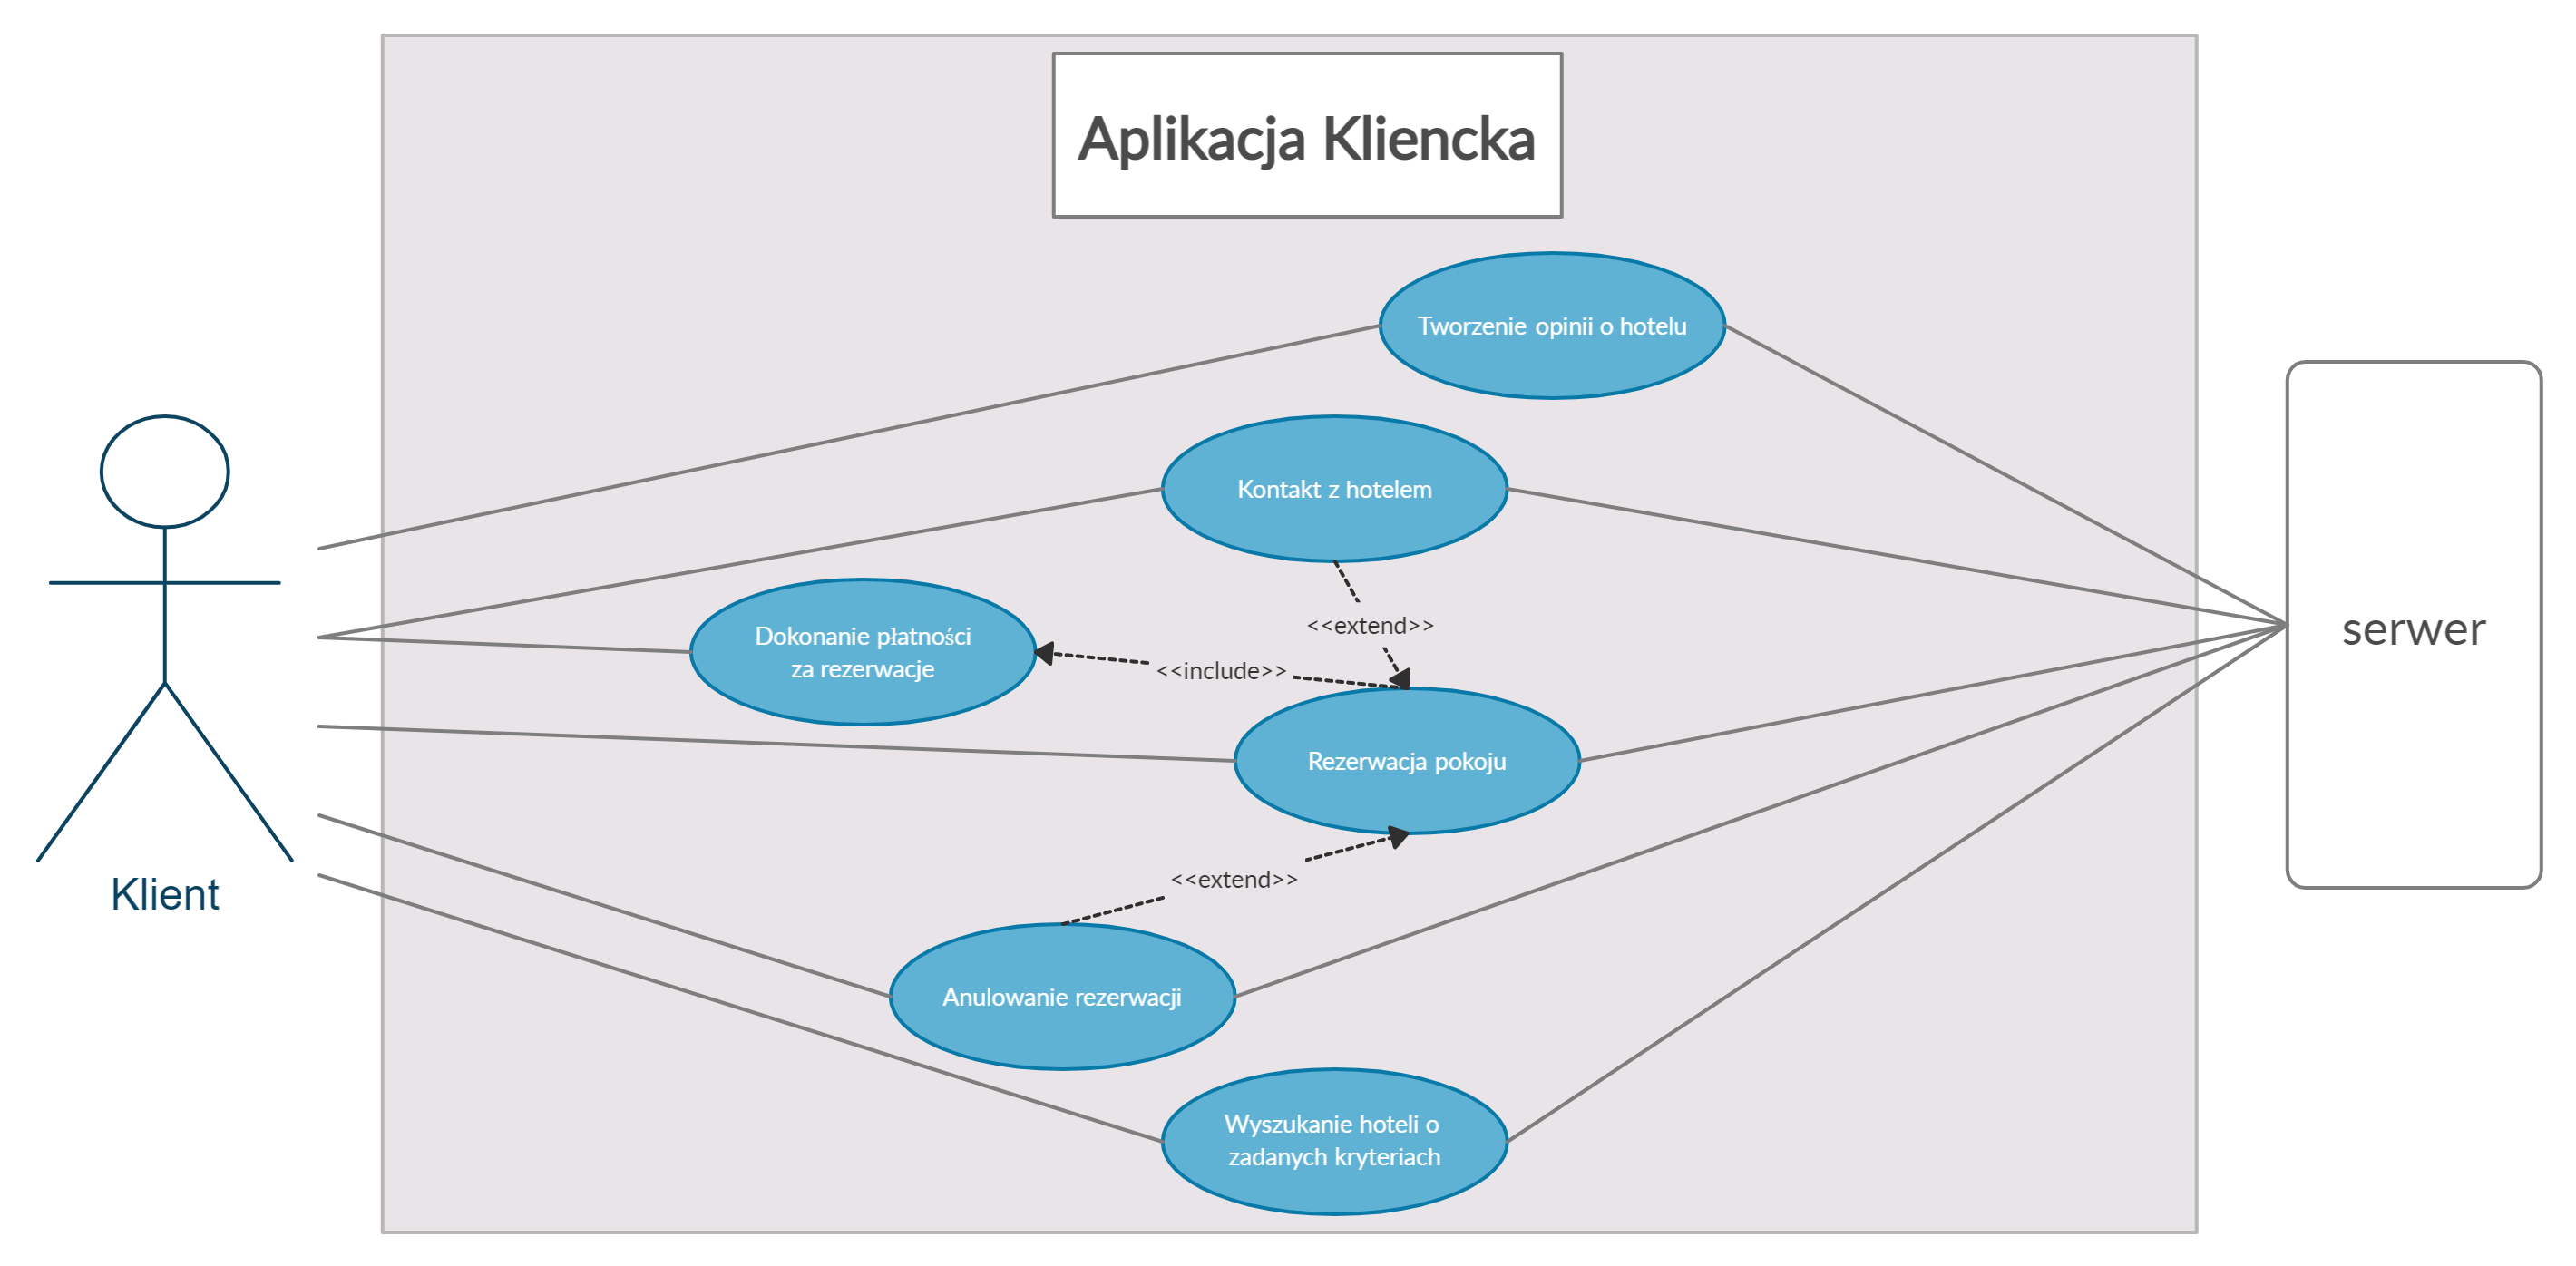
\includegraphics[width=\linewidth]{checkpoint1/Use cases - klient.png}
\indent W obrębie aplikacji klienckiej dowolny klient będzie mógł wyszukać interesujący go hotel lub hotele wysyłając zapytanie z podanymi przez niego kryteriami do serwera, zarezerwować interesujący go pokój (równocześnie opłacając daną rezerwację) lub zarządzać swoimi rezerwacjami - anulować je lub pozyskać dodatkowe informacje poprzez kontakt z hotelem, lub też zostawić opinię o danym hotelu po zakończonym pobycie.

\subsubsection{Hotel}
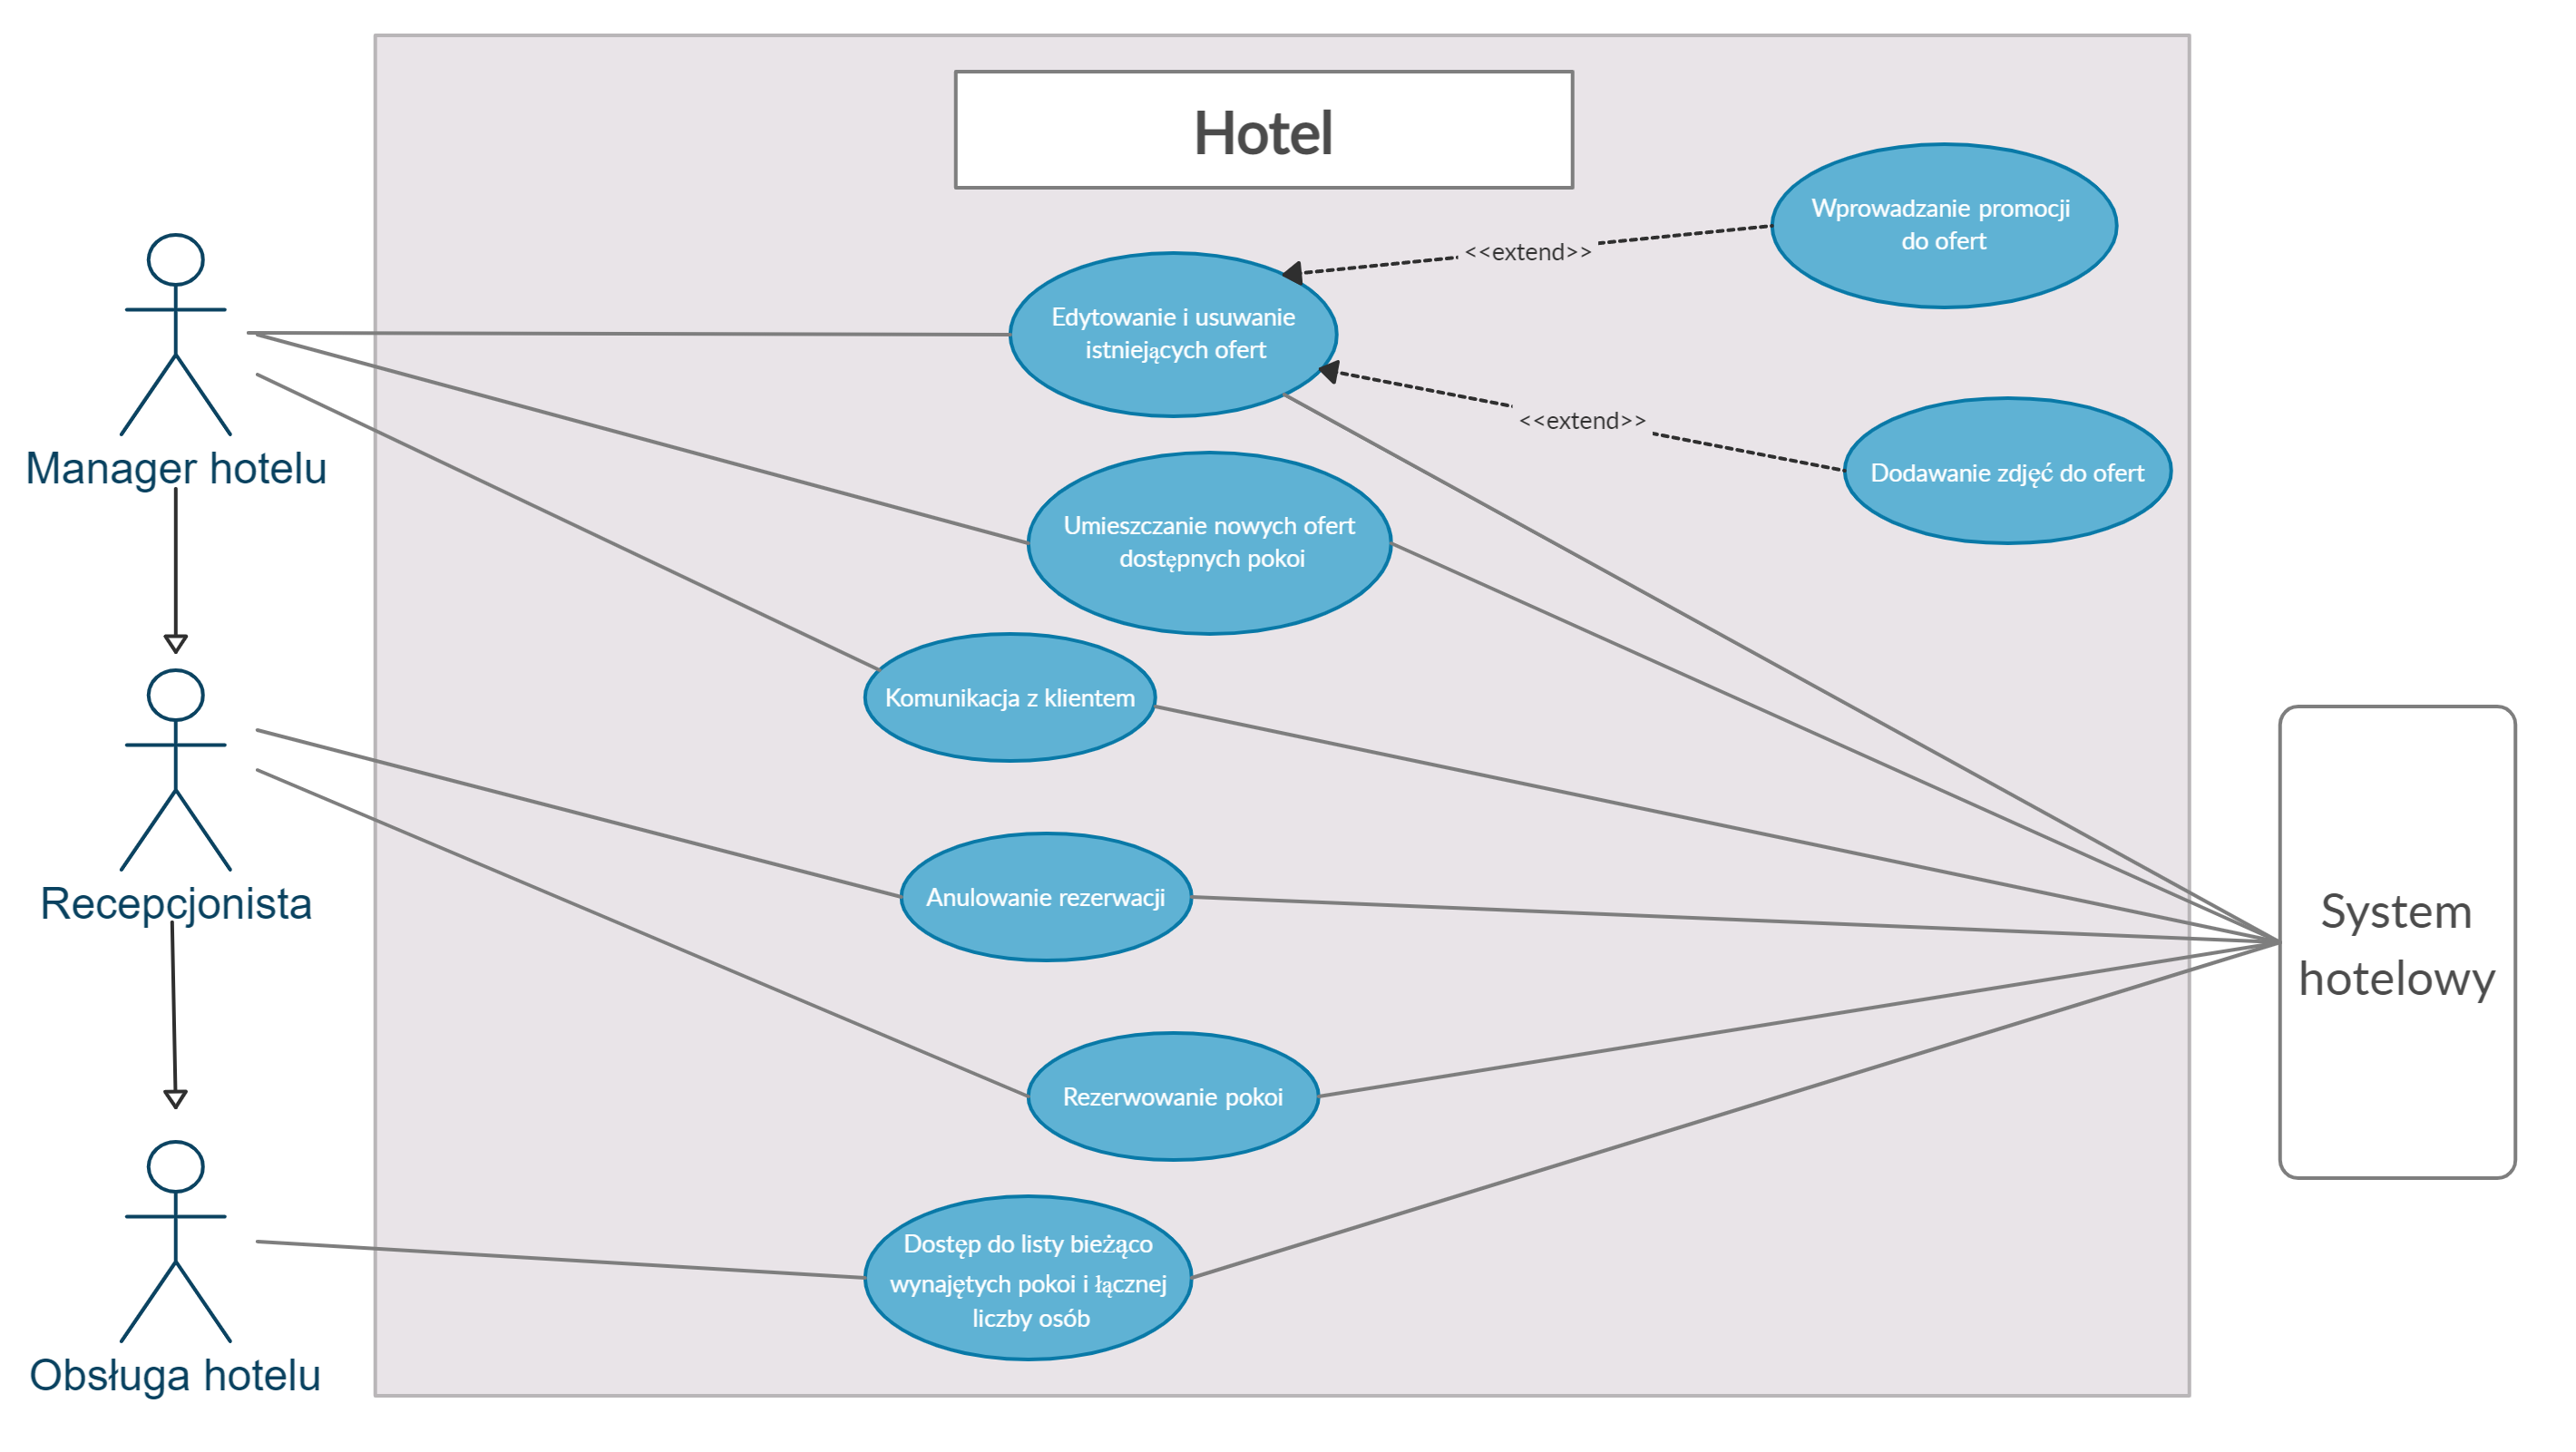
\includegraphics[width=\linewidth]{checkpoint1/Use cases - hotel.png}
\indent Moduł hotelowy wspomaga operowanie danym hotelem jego obsłudze poprzez system hotelowy. W obrębie systemu obsługa hotelu ma dostęp do listy obecnie wynajętych pokoi i łącznej liczby osób w celu np. wyznaczenia odpowiedniej pory posprzątania danych pokoi.
Recepcjoniści, oprócz posiadania tych samych uprawnień co obsługa, mogą dokonywać rezerwacji na rzecz klienta lub je anulować, jeśli zaistnieje taka potrzeba.
Z kolei dla managera danego hotelu, który ma najwyższe uprawnienia, zarezerwowane są możliwości dodania ofert do hotelu, (a zarazem ich edycji/aktualizacji np. umieszczenie zdjęć, opisu czy też ustalenie promocji), jak również bezpośrednia komunikacja z klientem.

\subsubsection{Serwer}
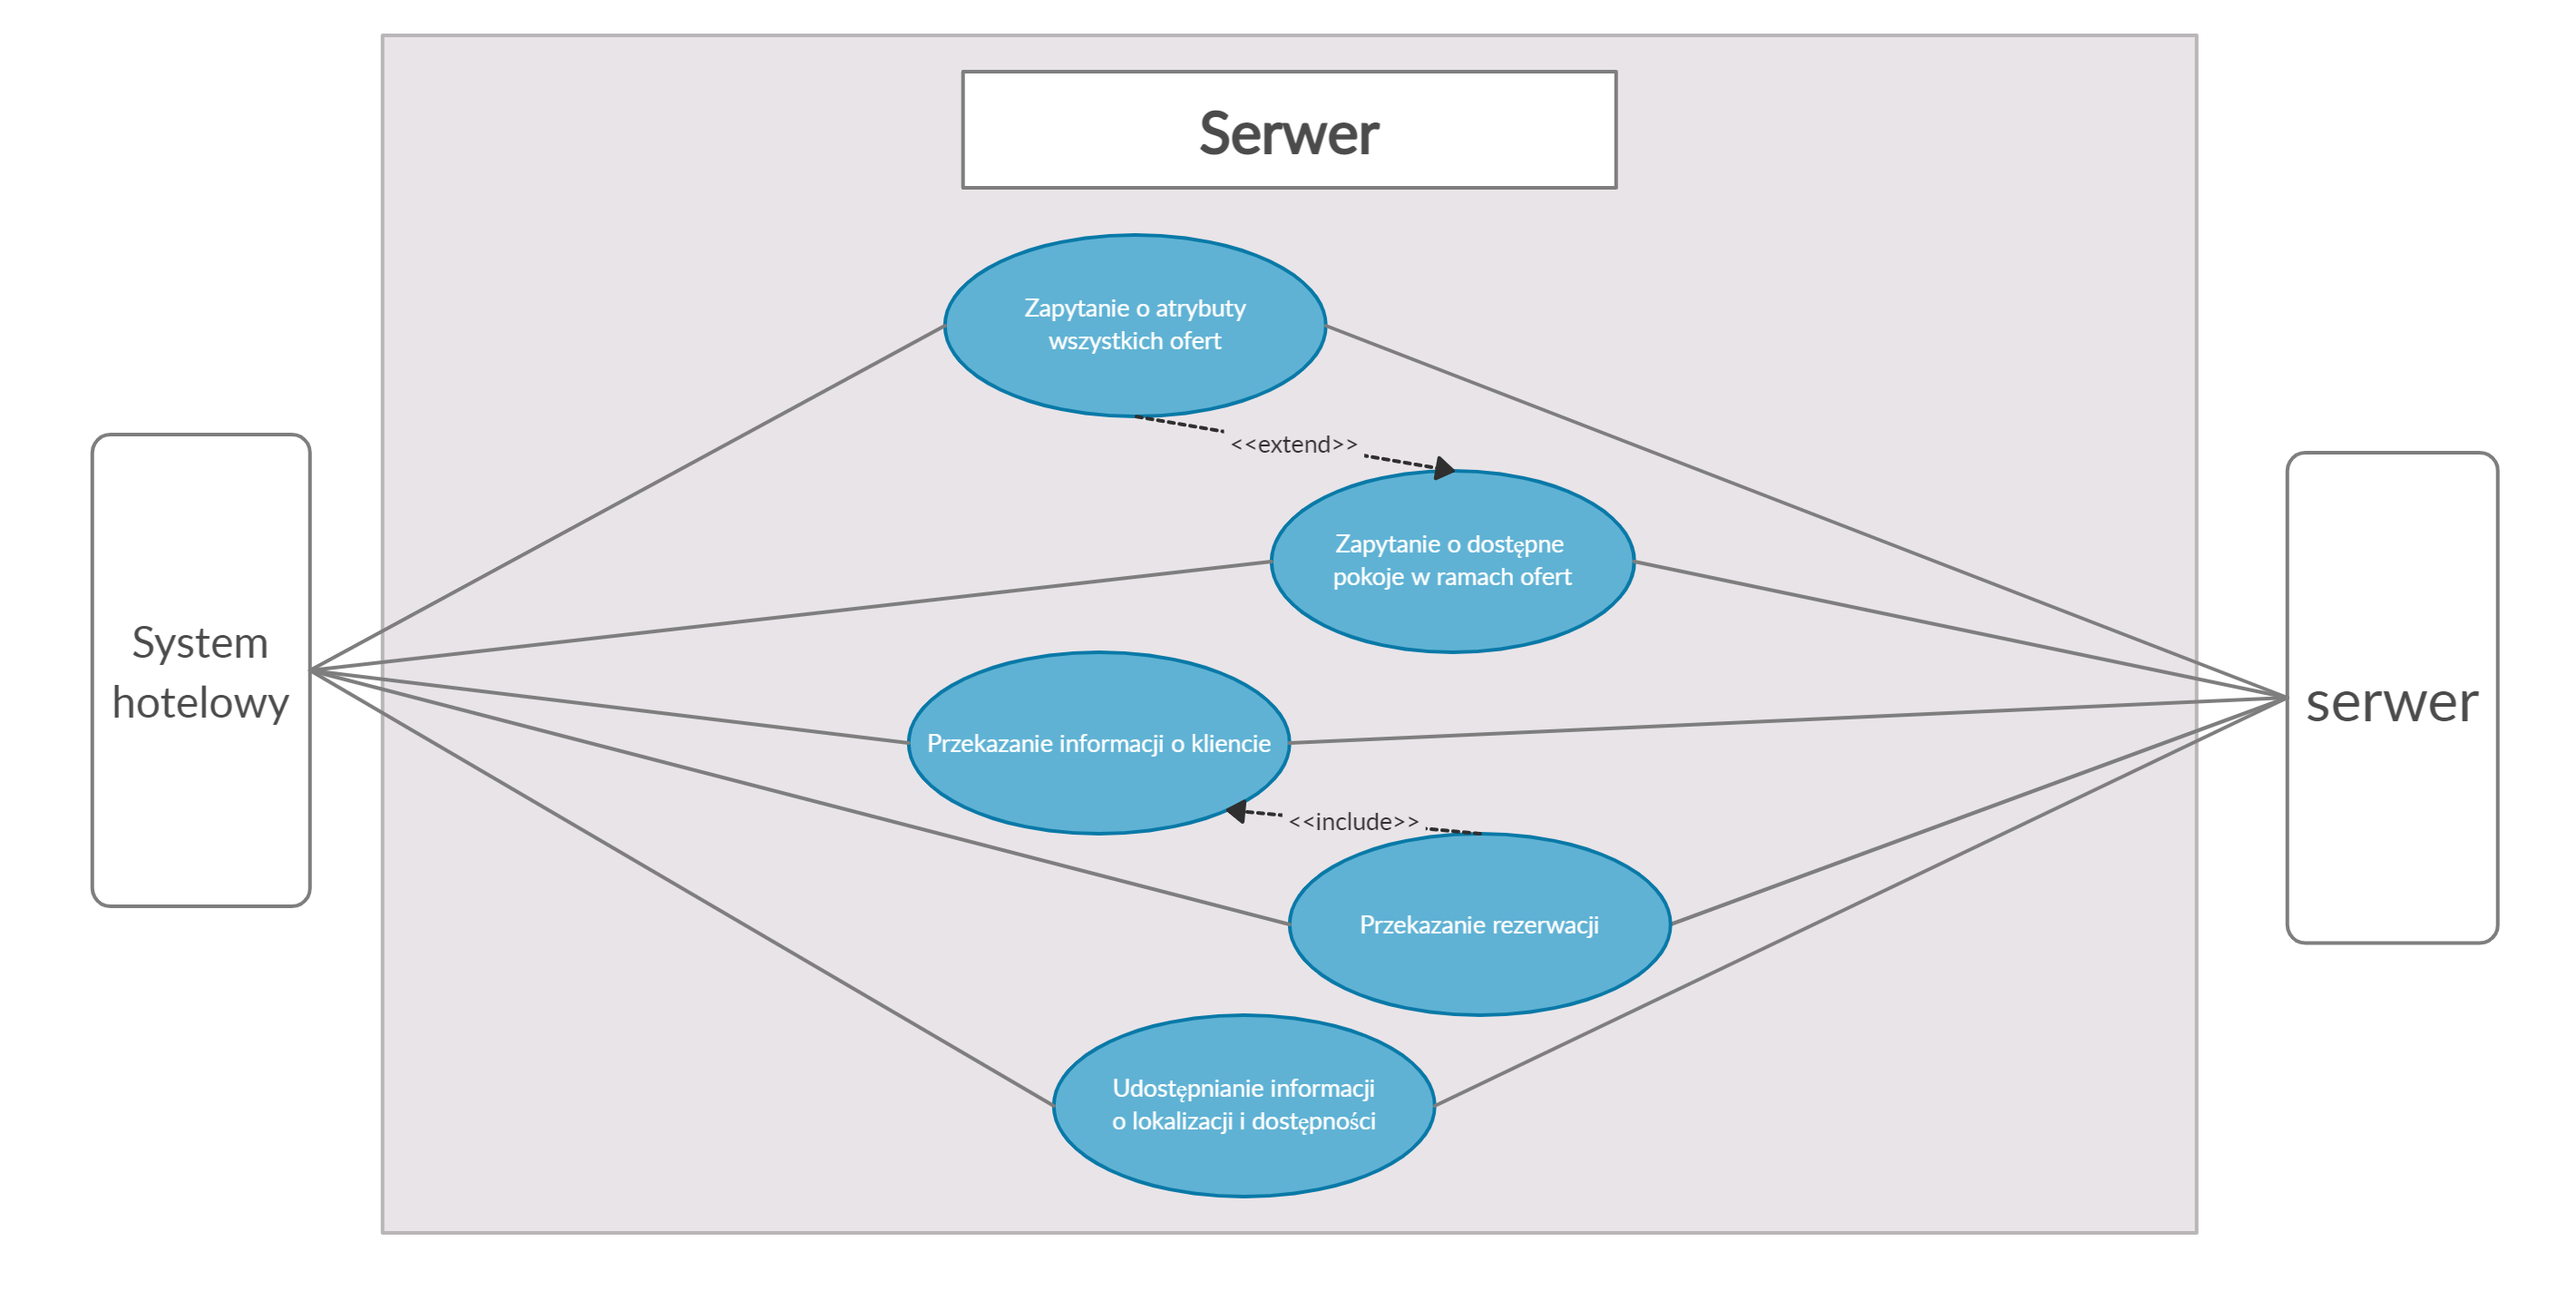
\includegraphics[width=\linewidth]{checkpoint1/Use cases - serwer.png}
\indent W module serwera przewidywane są funkcjonalności synchronizacji (udostępnienia) danych o lokalizacji i dostępności danego hotelu między serwerem a systemem hotelowym, przekazania infor\-macji o rezerwacji jakiegoś pokoju (w tym również danych o kliencie, który dany pokój postanowił zare\-zerwować) lub odpytania o dostępność pokoi w ramach ofert danego hotelu. Ostatnie zapytanie może zostać rozszerzone o atrybuty wszystkich dostępnych ofert danego hotelu. Są to funkcje niezbędne do prawidłowej wymiany informacji między systemem hotelowym a serwerem, a zarazem ich efektywnej pracy.

%\begin{center}
%    \begin{figure}[h!]
%    \centering
%    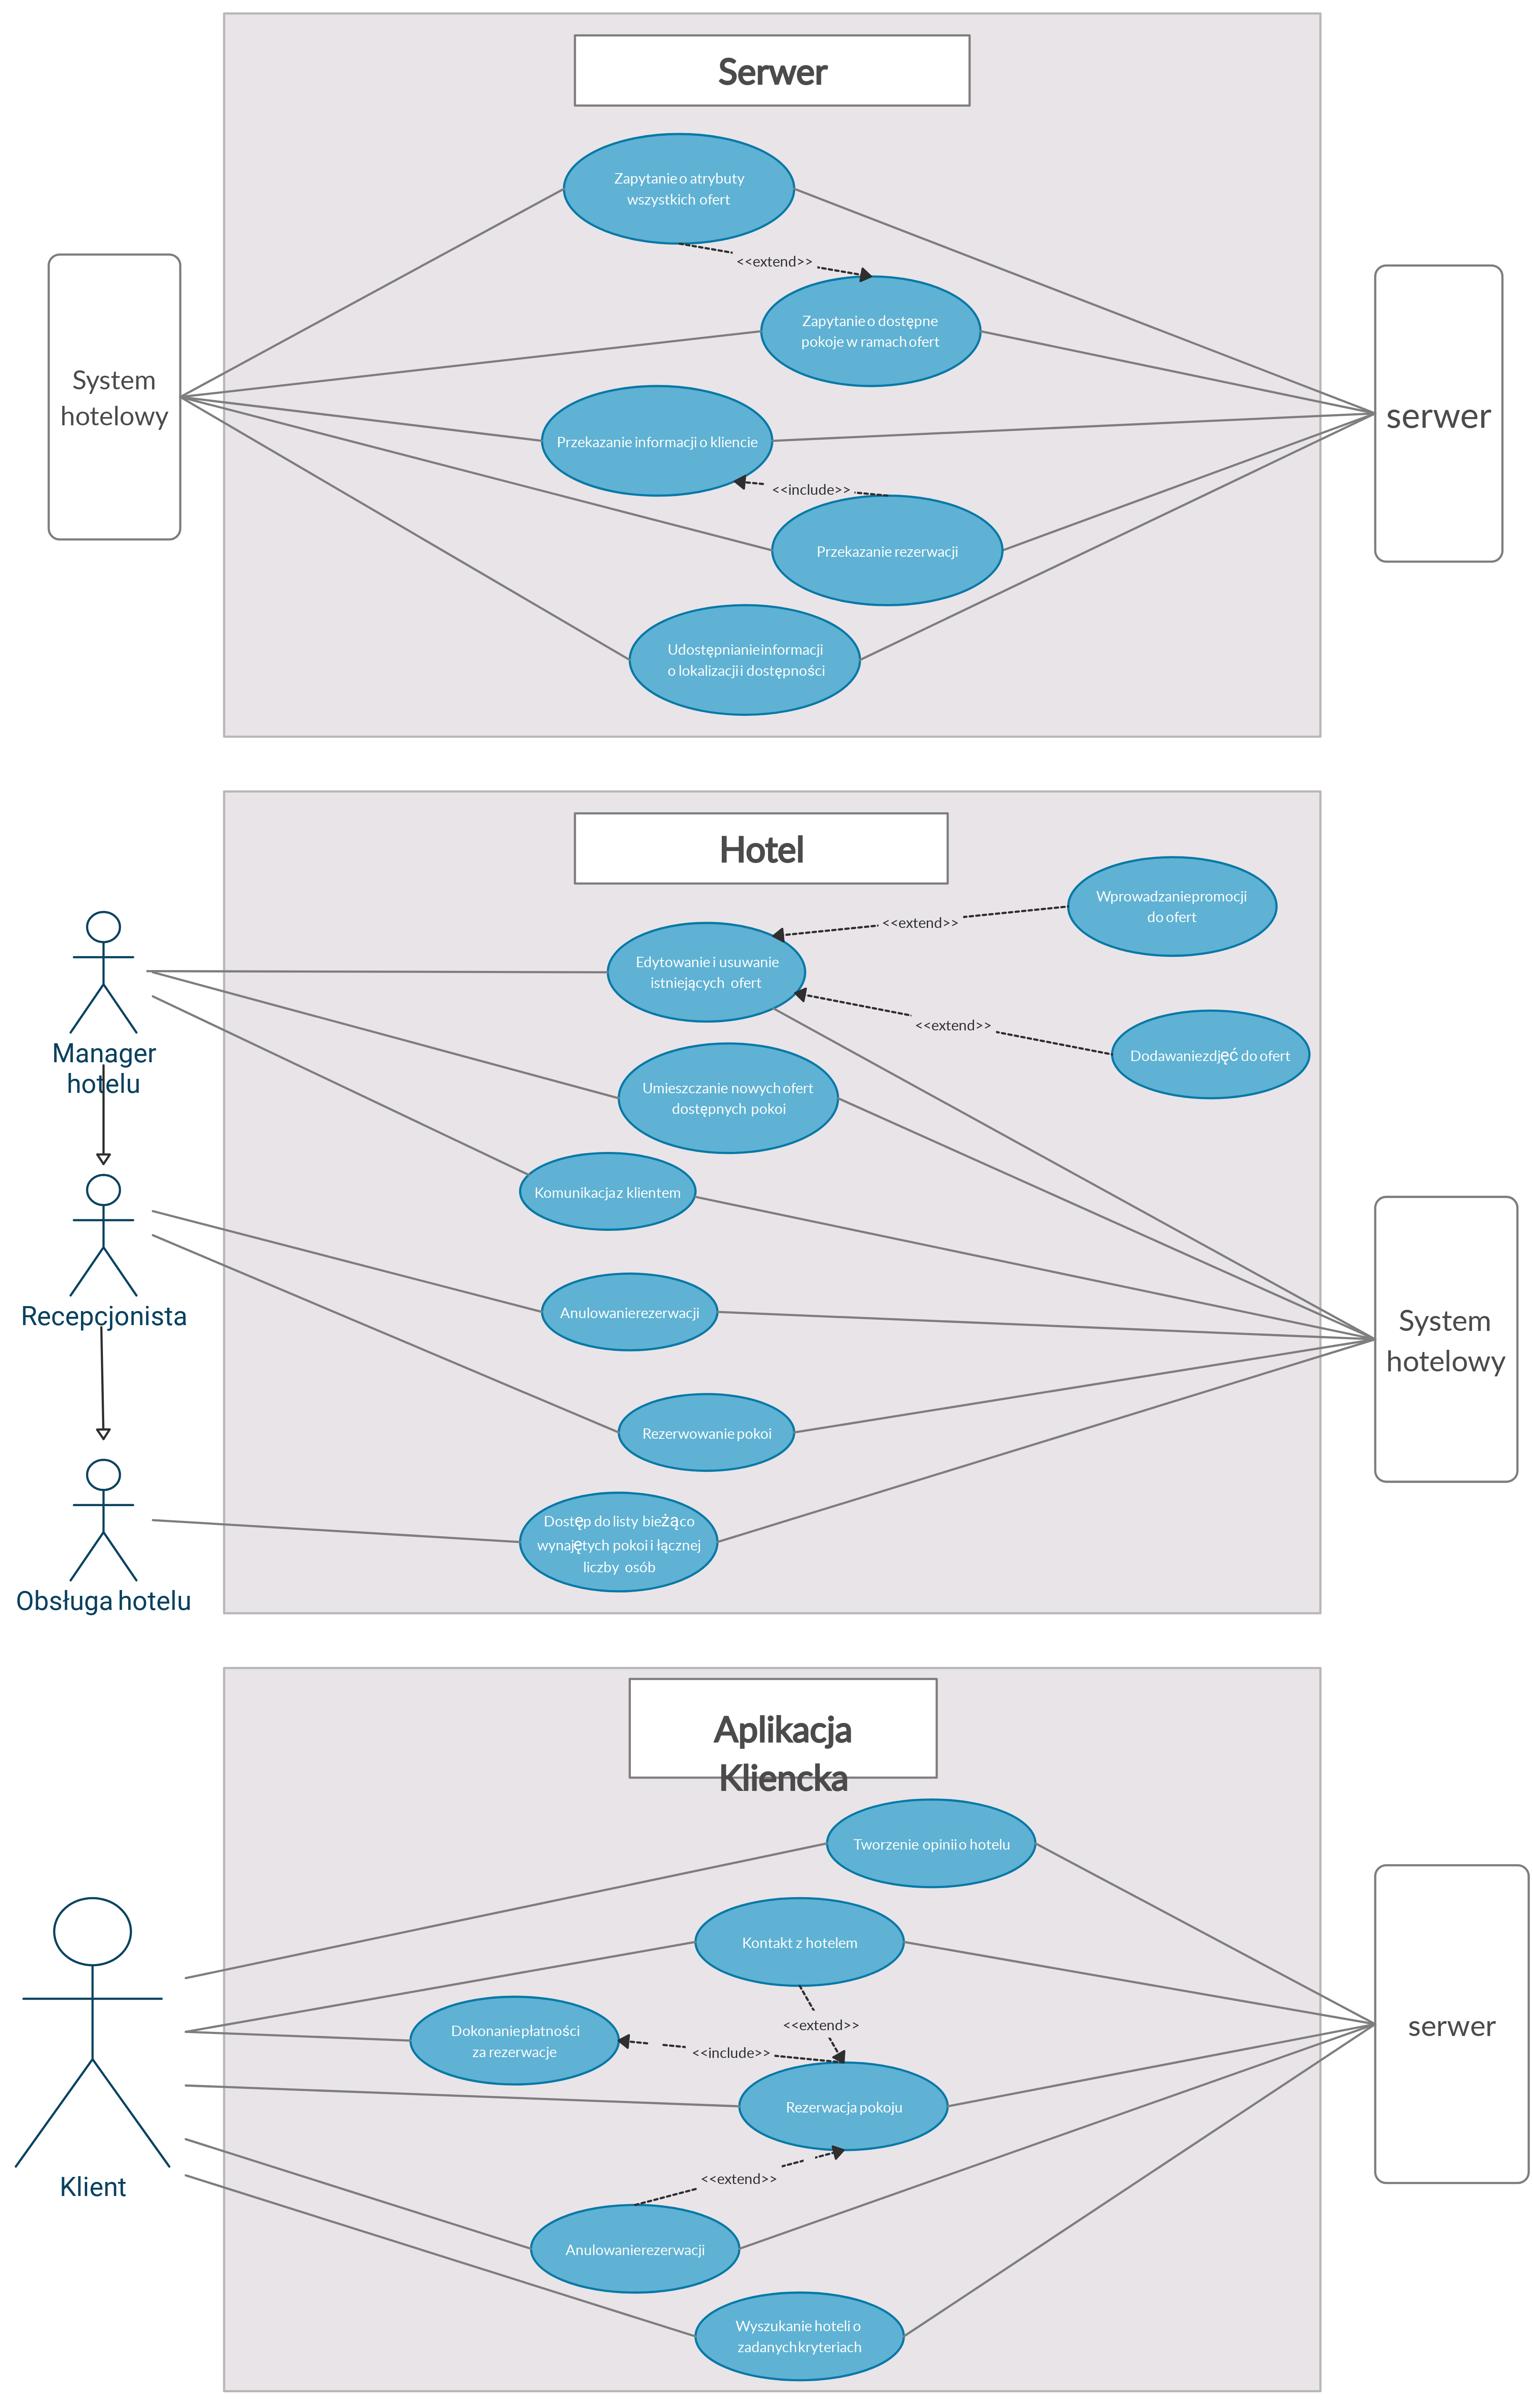
\includegraphics[scale=0.1]{Use.png}
%    \caption{UML}
%    \label{fig:UML}
%    \end{figure}
%\end{center}


\subsection{Przykładowe przypadki użycia (use cases)}
\subsubsection{Wyszukanie pokoju przez klienta}
\begin{flushleft}
\resizebox{\linewidth}{!}{%
\begin{tabular}{  |l|l| }
\hline
Nazwa: & Klient wyszukuje pokój\\
\hline
Krótki opis: & Na życzenie klienta do hoteli wysyłane jest zapytanie o pokoje spełniające dane kryteria \\
\hline
Warunki startowe: & Klient wybrał hotele i warunki jakie muszą spełniać pokoje\\
\hline
Warunki kończące: & Klient widzi listę pokoi spełniających warunki\\
\hline
Możliwe błędy & \makecell[l]{Przerwanie połączenia}\\

\hline
W razie błędu: & \makecell[l]{Informacja o błędzie połączenia}\\
\hline
Aktorzy: & Klient, serwer, system hotelowy\\
\hline
Zapalnik: & Klient wysyła prośbę do serwera z podanymi atrybutami filtrowania (region, ocena itp.) \\
\hline
Standardowy proces: & \makecell[l]{(1) Klient wysyła zapytanie\\
(2) Serwer odsyła listę do klienta wraz z dołączonymi do ofert opiniami\\
(3) Klientowi wyświetlona jest lista pokoi}\\
\hline
Proces alternatywny: & \makecell[l]{Zerwanie połączenia, może nastąpić w każdym kroku.\\
Klient jest informowany o zaistniałych problemach z połączeniem }\\
\hline
\end{tabular}}
\end{flushleft}

W przypadku wyszukiwania przez klienta interesujących go ofert musi on najpierw wybrać hotele oraz parametry pokoi, następnie wysłać zapytanie z danymi parametrami do serwera.
Ten następnie na podstawie własnych, lokalnych danych dotyczących wszystkich modułów hotelowych przeszukuje oferty i wysyła listę, która następnie zostaje pokazana klientowi.
Jeśli w dowolnym momencie interakcji wystąpią problemy z połączeniem, użytkownikowi zostanie wyświetlona odpowiednia informacja o braku połączenia.
W przypadku gdy któraś instancja systemu hotelowego nie jest osiągalna przez serwer agregujący, klientowi zostanie wyświetlona odpowiednia informacja.

\subsubsection{Dodanie nowej oferty pokoju do systemu przez managera hotelu}
\begin{flushleft}
\resizebox{\linewidth}{!}{%
\begin{tabular}{  |l|l| }
\hline
Nazwa: & Manager umieszcza nową ofertę\\
\hline
Krótki opis: & Manager umieszcza w bazie hotelowej nową ofertę \\
\hline
Warunki startowe: & Serwer hotelowy działa\\
\hline
Warunki kończące: & Nowa oferta jest w bazie\\
\hline
Możliwe błędy & Brak wymaganego pola \\
\hline
W razie błędu: & Wyświetlić komunikat o błędzie i nie dodawać oferty do bazy\\
\hline
Aktorzy: & Manager i system hotelowy\\
\hline
Zapalnik: & Próba dodania oferty do bazy \\
\hline
Standardowy proces: & \makecell[l]{(1) Manager stwierdza że chce wprowadzić nową ofertę\\
(2) Manager wprowadza dane do formularza\\
(3) Potwierdza zakończenie\\
(4) Formularz został wypełniony poprawnie\\
(5) System hotelowy zgodnie z formularzem wkleja nową ofertę do bazy danych\\
(6) System hotelowy synchronizuje się z modułem serwerowym\\ co skutkuje pojawieniem się oferty w bazie danych serwera }\\
\hline
Proces alternatywny: & \makecell[l]{(4) Formularz nie został wypełniony poprawnie\\
(5) Manager zostaje poinformowany o błędzie i oferta nie jest dodawana}\\
\hline
\end{tabular}}
\end{flushleft}

W sytuacji, kiedy wymagane jest dodanie nowej oferty pokoju, manager hotelu wypełnia odpowiedni formularz z parametrami pokoju. Jeśli któreś pole nie zostało wypełnione poprawnie (np. pola wymagane są puste lub wprowadzone dane są nieprawidłowe), aplikacja zwraca błąd i nie dodaje oferty, w przeciwnym wypadku system hotelowy dodaje ofertę do swojej bazy danych zgodnie z wypełnionym formularzem. W późniejszym czasie baza danych hotelu zostanie zsynchronizowana z serwerem i dane oferty pojawią się w bazie danych serwera agregującego.

\subsubsection{Rezerwacja pokoju przez klienta}
\begin{flushleft}
\resizebox{\linewidth}{!}{%
\begin{tabular}{|l|l|}
\hline
Nazwa: & Rezerwacja pokoju\\
\hline
Krótki opis: & Klient dokonuje rezerwacji w wybranym hotelu i wybranej oferty \\
\hline
Warunki startowe: & Wybrana przez klienta oferta jest dostępna w oparciu o dane serwera \\
\hline
Warunki kończące: & Rezerwacja pokoju przez klienta na wybrany okres\\
\hline
Możliwe błędy & \makecell[l]{Niedostępność oferty wynikająca z braku synchronizacji między hotelem a serwerem \\ Płatność za rezerwacje nie jest widoczna przez hotel pomimo zgłoszenia zakończenia procesu płatności przez klina}\\
\hline
W razie błędu: & \makecell[l]{Wyświetlić komunikat o błędzie i zakończyć proces tworzenia rezerwacji\\Przeprowadznie synchronizacji po stronie serwera z hotelem}\\
\hline
Aktorzy: & Klient, serwer, hotel\\
\hline
Zapalnik: & Próba rezerwacji pokoju \\
\hline
Standardowy proces: & \makecell[l]{ (1) Klient wyszukuje oferty spełniającą jego oczekiwania\\
(2) Klient wysyła żądani do serwera o utworzenie rezerwacji \\
(3) Serwer sprawdza dostępność oferty w wybranym przedziale czasowym w oparciu o lokalne dane \\
(4) Rezerwacja jest przekazywana hotelowi i sprawdzana jest ponowni dostępność oferty\\
(5) Hotel tworzy wpis o rezerwacji, przesyła serwerowi\\ informacji o płatności, która musi być zrealizowana przez klienta \\
(6) Klient dokonuj płatności i informuje o tym serwer \\
(7) Serwer informuje hotel o ukończonej płatności\\
(8) Hotel sprawdza czy rezerwacja została opłacona\\ i czy pieniądze zostały poprawnie przelane na konto bankowe hotelu \\
(9) Hotel odsyła informację o sukcesie finalizacji tworzenia rezerwacji do serwera \\
(10) Serwer tworzy wpis w lokalnej bazie danych o nowo utworzonej rezerwacji \\
(11) Wysyłany jest komunikat do klienta o poprawnym utworzeniu nowej rezerwacji }\\
\hline
Proces alternatywny: & \makecell[l]{(2.5) Rezerwacja nie jest możliwa (serwer stwierdza brak dostępności oferty\\w oparciu o lokalne dane)\\
(3) Rezerwacja zostaje anulowana\\
(4) Klient zostaje poinformowany o niepowodzeniu rezerwacji\\
(8.5) Hotel informuje serwer o błędzie płatności\\
(9) Serwer informuje klienta o błędzie płatności\\ oraz konieczności kontaktu z hotelem w celu wyjaśnienia tego błędu.
}\\
\hline
\end{tabular}}
\end{flushleft}

Kiedy klient wybrał interesującą go ofertę rezerwacji, wysyła informację o próbie rezerwacji pokoju. Jeżeli serwer stwierdzi, że oferta rezerwacji pokoju nie jest dostępna, to zwracana jest informacja z błędem i nie jest wykonywana rezerwacja. W przeciwnym przypadku serwer przekierowuje prośbę utworzenia rezerwacji do hotelu, gdzie dostępność rezerwacji jest ponownie sprawdzana. Jeśli oferta jest dostępna w wybranym przedziale czasowym tworzona jest lokalna rezerwacja po stronie hotelu i odsyłany jest identyfikator płatności za tą ofertę. Klient musi opłacić swoją rezerwację, po czym odsyła do serwera informację o zakończonym procesie płatności. Po potwierdzeniu ukończonej płatności przez hotel, wpis o rezerwacji jest tworzony na serwerze i zwracana jest klientowi informacja o zakończeniu procesu tworzenia rezerwacji. W przypadku niepowodzenia płatności (np. pieniądze nie zostały zaksięgowane na koncie hotelu) serwer informuje klienta o konieczności kontaktu z hotelem w celu wyjaśnienia tej sytuacji. Jeśli natomiast hotel stwierdzi brak dostępności oferty wysyłana jest informacja o błędzie serwerowi, co świadczy o desynchronizacji danych między hotelem i serwerem. Odsyłany jest wówczas klientowi błąd mówiący o braku dostępności oferty w wybranym okresie czasowym.

\section{Diagramy Klas}
We wszystkich trzech modułach Systemu zdecydowaliśmy się zastosować rozdział części odpowiada\-jącej za połączenie między modułami (klasy nazwane \texttt{*Connection}) od części odpowiadającej za wysokopo\-ziomowe akcje (czyli metody zawarte w klasach \texttt{*Manager}). Dzięki takiemu krokowi rozdzie\-lamy obsługę błędów związanych z połączeniem od walidacji formularzy i błędów związanych z poprawnością wprowadzonych danych. Klasa \texttt{*Connection} pracuje na danych, które są poprawne. W odpowiedzialności klasy \texttt{*Manager} znajduje się dbanie o poprawną komunikację – w związku z tym również wywoływanie odpowiednich metod klasy \texttt{*Connection}.\\
Ponadto w modułach serwerowym oraz hotelowym – które dysponują swoimi lokalnymi bazami danych – wyróżniono klasę \texttt{DataManager}, będącą \textbf{wyłącznym} pośrednikiem w pobieraniu informacji z tej bazy. Z tego względu \texttt{DataManager} został oznaczony na diagramie jako klasa silnie agregująca obiekty tych typów, które może zwrócić – niezależnie od faktycznej technologii, która została użyta do implementacji tej części (np. SQL czy ORM).

\subsection{Aplikacja Kliencka}
\begin{center}
    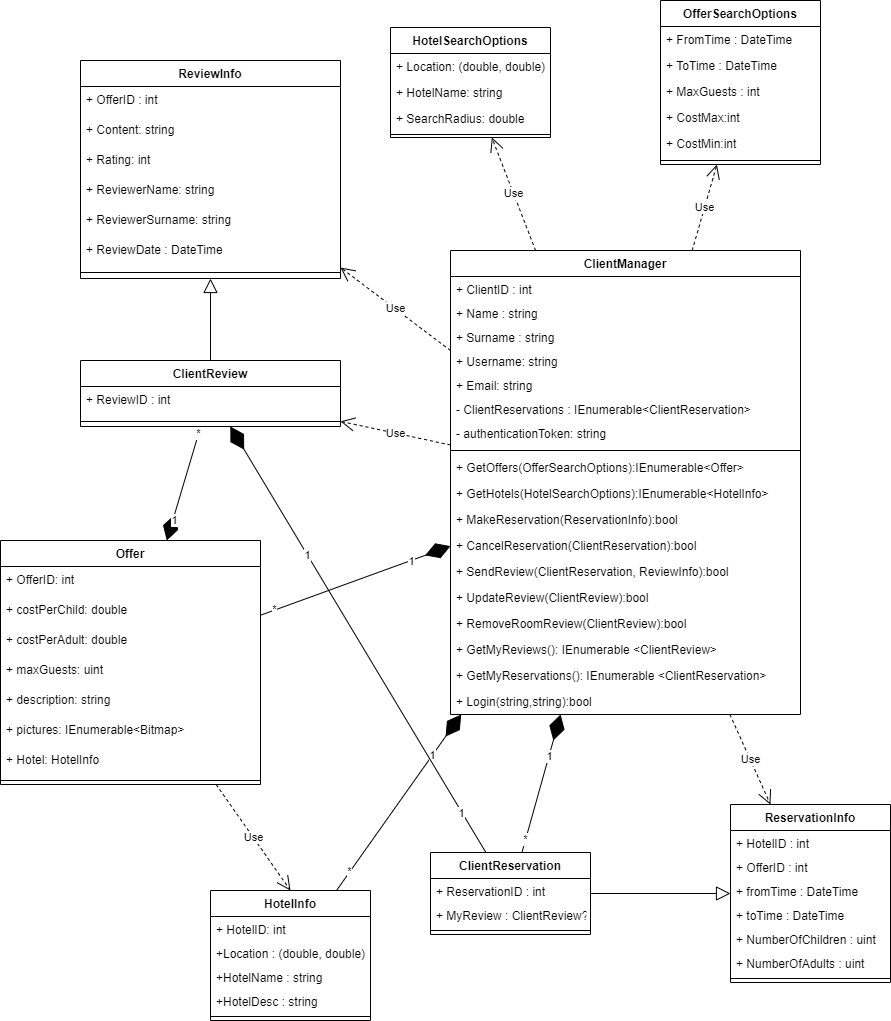
\includegraphics[scale=0.45]{checkpoint1/IO Klasy-Client_App_Module.png}
\end{center}

\subsubsection{ClientManager}
\indent \indent Klasa ta zawiera implementacje metod, które są wywoływane z poziomu UI użytkownika. Zawiera odpowiednie metody służące do autentykacji oraz dane o użytkowniku.
\begin{itemize}
    \item Login \\
    Funkcja wywoływana w czasie logowania się użytkownika do systemu.
    Przekazywane argumenty to w kolejności login i hasło.\\
    Zwraca boola czy operacja się powiodła i w przypadku powodzenia pobiera informacje o zalogowanym kliencie.
    \item GetOffers\\
    Funkcja pobiera informacje o ofertach w systemie zgodnie z kryteriami filtracji użytkownika w postaci obiektu OfferSearchOptions przekazanego do funkcji.
    \item GetHotels\\
    Funkcja pobiera informacje o hotelach w systemie zgodnie z kryteriami filtracji użytkownika w postaci obiektu HotelSearchOptions przekazanego do funkcji.
    \item MakeReservation\\
    Funkcja próbuje dodać do systemu rezerwację o parametrach do niej przekazanych.\\
    Zwraca informację czy operacja się powiodła.
    \item CancelReservation\\
    Funkcja usuwa z systemu rezerwację przekazaną jako parametr.\\
    Zwraca informację czy operacja się powiodła.
    \item RemoveRoomReview\\
    Funkcja usuwa z systemu opinię przekazaną jako parametr.\\
    Zwraca informację czy operacja się powiodła.
    \item UpdateReview\\
    Funkcja aktualizuje już istniejącą Review w systemie (zmiana oceny lub opisu).\\
    Zwraca informację czy operacja się powiodła.
    \item SendReview\\
    Funkcja dodaje do systemu nową opinię dotyczącą Oferty której Id zostało przekazane jako parametr.
    Zwraca informację czy operacja się powiodła.
    \item GetMyReviews\\
    Funkcja zwraca listę opinii utworzonych przez zalogowanego klienta.
    \item GetMyReservations\\
    Funkcja zwraca listę rezerwacji złożonych przez zalogowanego klienta.
\end{itemize}

\subsubsection{HotelInfo}
Klasa przetrzymuje informacje o hotelu.

\subsubsection{HotelSearchOptions}
Klasa trzyma w sobie wymagania jakie muszą spełniać hotele wyszukiwane przez klienta.\\
Używana tylko przy wyszukiwaniu.

\subsubsection{Offer}
Klasa przetrzymująca wszystkie informacje o ofercie.

\subsubsection{OfferSearchOptions}
Klasa trzyma w sobie wymagania, które musi spełniać oferta wyszukiwana przez klienta.\\
Używana tylko przy wyszukiwaniu.

\subsubsection{ReservationInfo}
Klasa trzyma informacje o rezerwacji bez identyfikatora rezerwacji i ewentualnej opinii.

\subsubsection{ClientReservaton}
Klasa trzyma wszystkie informacje o rezerwacji klienta wraz z opcjonalną opinią.

\subsubsection{ReviewInfo}
Klasa zawierająca informacje o recenzji bez jej identyfikatora.

\subsubsection{ClientReview}
Klasa przetrzymująca wszystkie informacje o opinii.

\subsection{Moduł hotelowy}
\begin{center}
    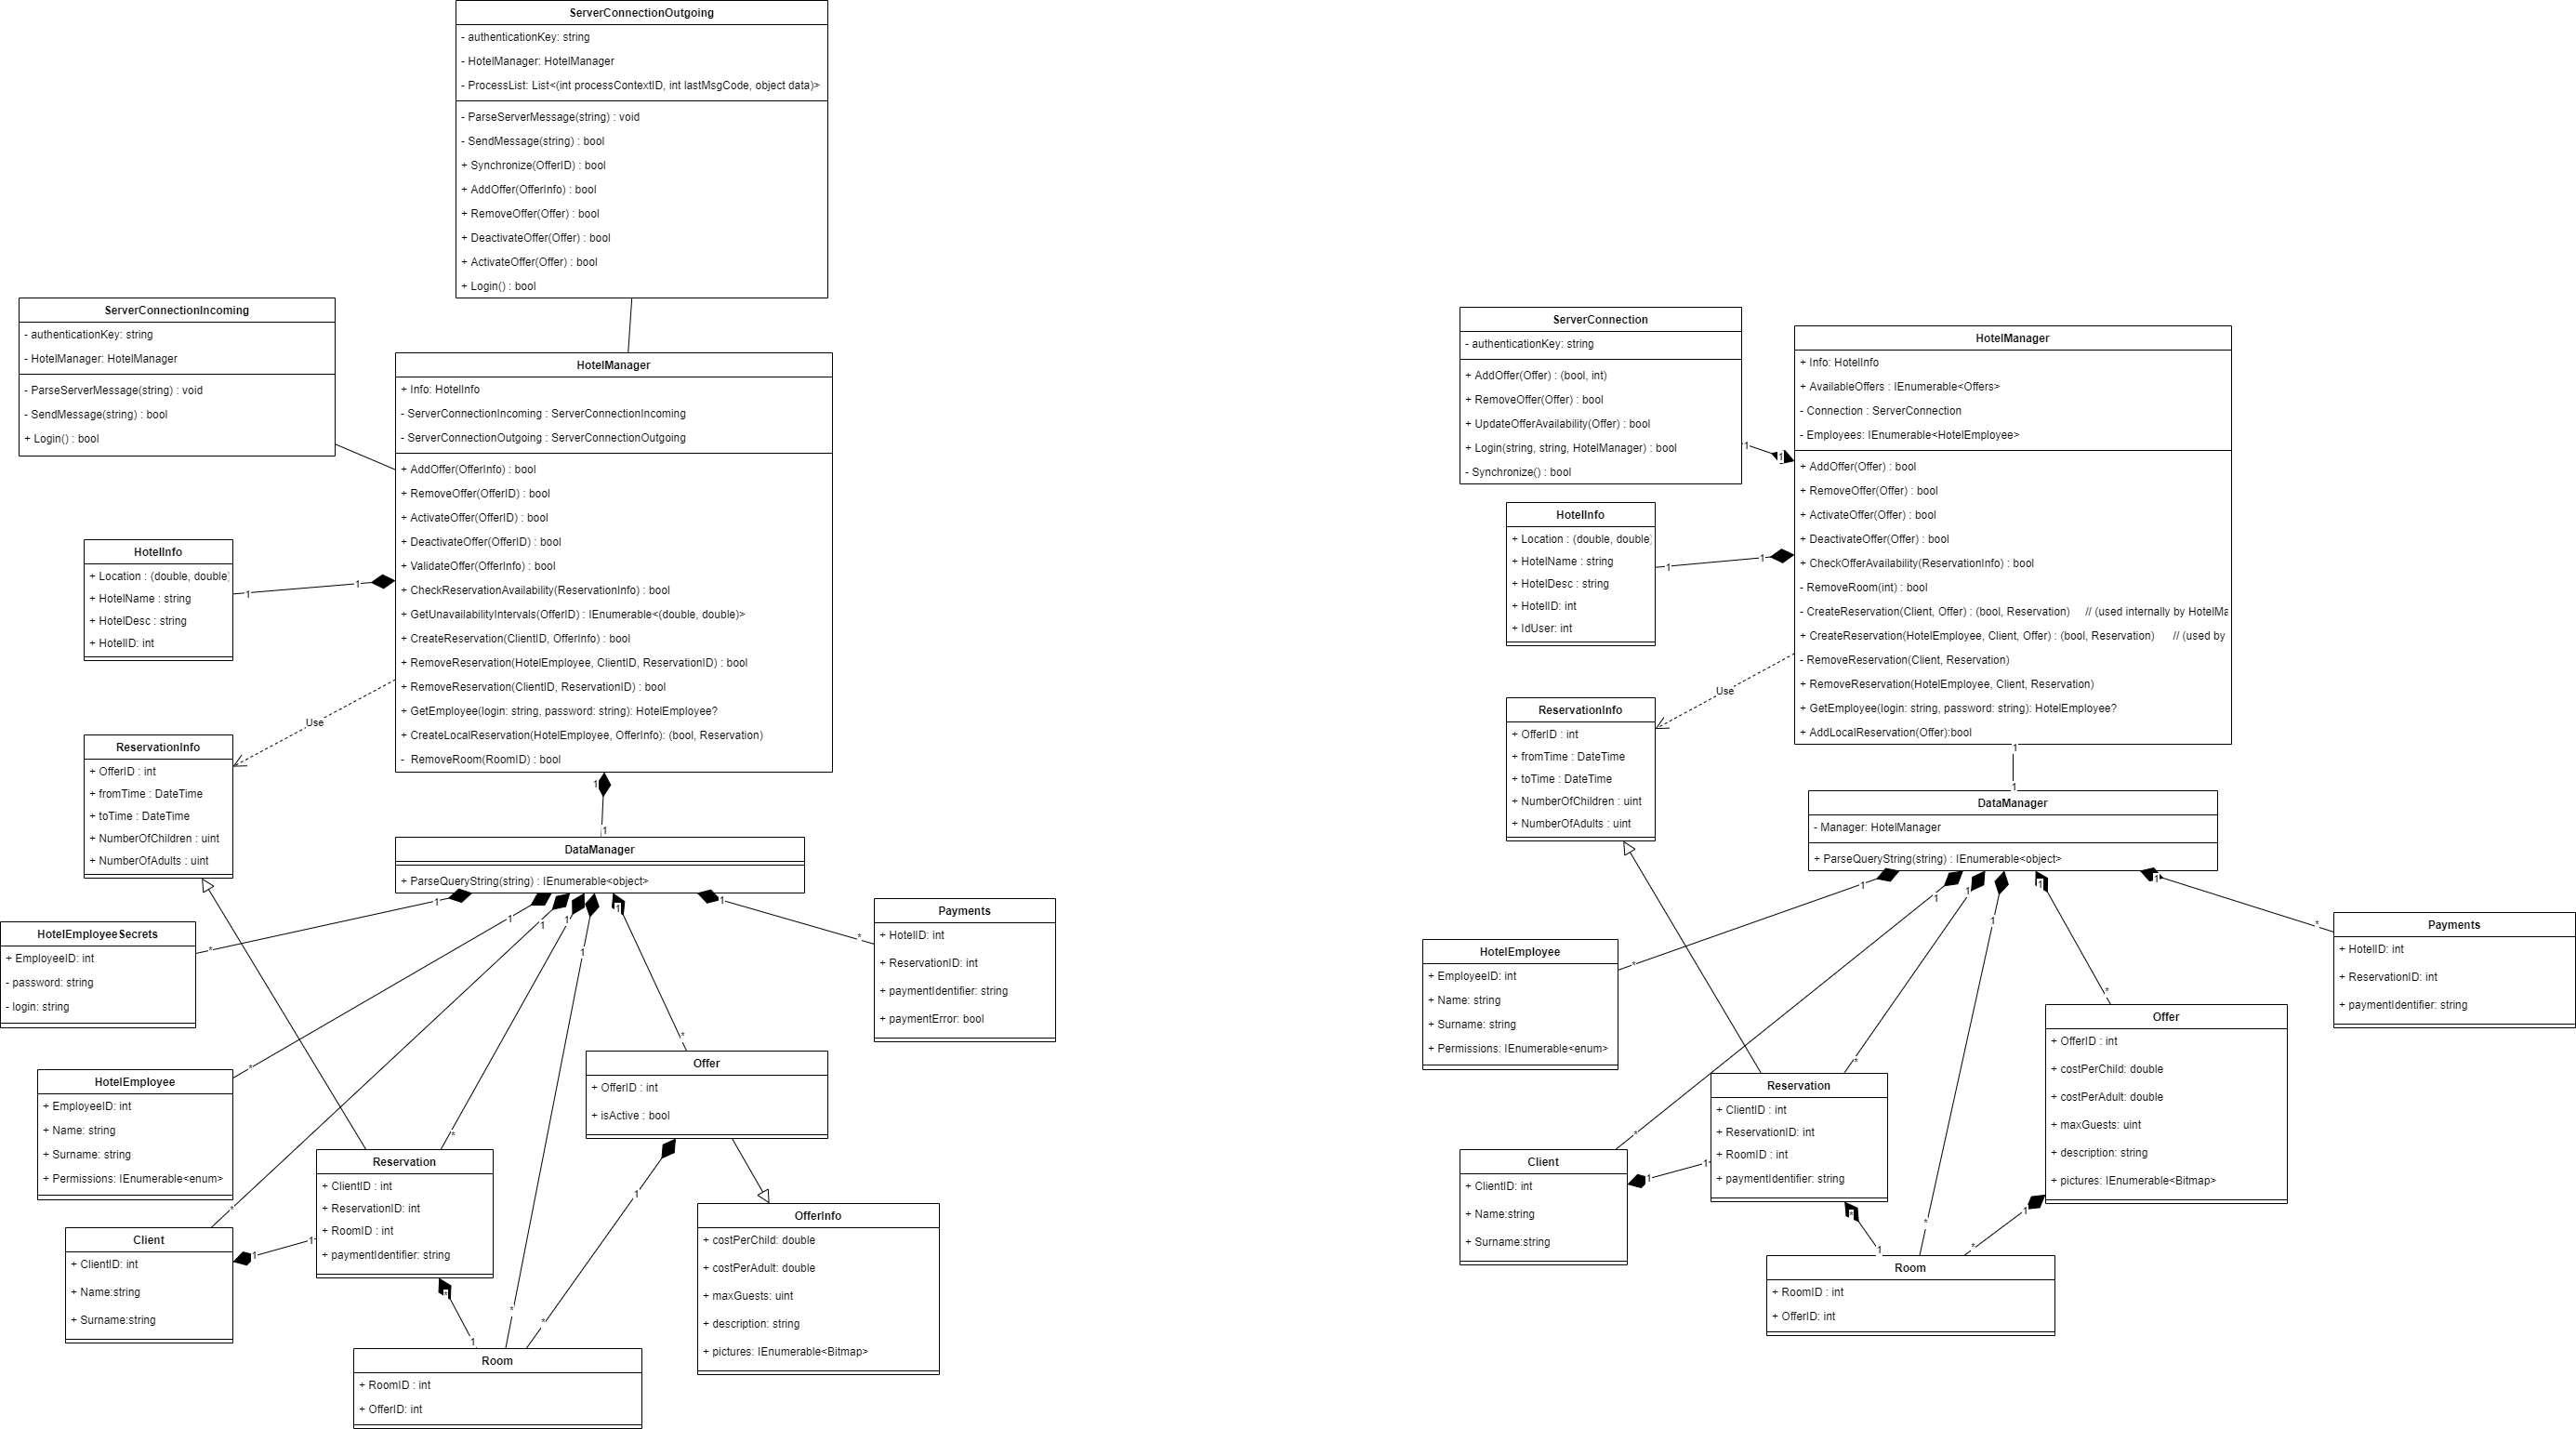
\includegraphics[scale=0.36]{checkpoint1/IO Klasy-Hotel_Module.png}
\end{center}

\subsubsection{OfferInfo}
Klasa przechowuje informacje opisujące daną ofertę bez informacji o jej identyfikatorze oraz stanu dotyczącego aktywności.

\subsubsection{Offer}
Klasa przechowuje informacje dotyczące różnych rodzajów ofert, jakie proponuje właściciel hotelu swoim potencjalnym klientom. Ponadto przechowywana jest informacja o tym czy oferta jest aktywna oraz jej identyfikator.

\subsubsection{Room}
\texttt{Pokój} jest klasą, która reprezentuje fizyczny pokój obecny w budynku hotelowym. Jego identyfikacja leży całkowicie w gestii zarządcy hotelowego. Ma odwołanie do \texttt{Offer}, w ramach której jest przedsta\-wiany na stronie.

\subsubsection{Client}
Reprezentuje klienta, którego konto istnieje w systemie rezerwacji pokoi.

\subsubsection{Reservation}
Przechowuje informacje dotyczące rezerwacji klienckiej razem z ID pokoju oraz ID oferty. Ponadto przechowywany jest identyfikator płatności rezerwacji w celu umożliwienia anulowania rezerwacji i zwrotu pieniędzy.

\subsubsection{ReservationInfo}
Przechowuje szczegóły dotyczące pojedynczej, potwierdzonej rezerwacji, czyli daty od kiedy do kiedy ma ona trwać, oraz liczbę gości w jej ramach.

\subsubsection{HotelEmployee}
Reprezentuje członka personelu hotelowego, który posiada dostęp do części danych w systemie. Zakres dostępu oraz ograniczenia zdefiniowane są przez pole \textbf{Permissions}, które zawiera zbiór zdefiniowanych przez managera stałych typu enum.

\subsubsection{HotelEmployeeSecrets}
Reprezentuje dane stanowiące podstawę do autentykacji pracownika hotelowego (dane z tabeli zawierającej obiekty tego typu są używane bezpośrednio przy logowaniu się przez personel do systemu). Ze względów bezpieczeństwa informacje o loginach i hasłach pracowników zawarte są w osobnej tabeli do której dostęp jest stosownie chroniony.

\subsubsection{Payments}
Reprezentuje dane dotyczące rezerwacji, które nie zostały jeszcze opłacone. W momencie poprawnego opłacenia rezerwacji usuwane są rekordy z tej tabeli.

\subsubsection{DataManager}
Klasa pośrednicząca w wydobywaniu informacji z bazy danych. W tym celu używa jej HotelManager. Posiada jedną metodę – \textbf{ParseQueryString(string)}, która przyjmuje kwerendę do sparsowania w języku bazy, np SQL. Ze względu na to, że pobranie danych możliwe jest wyłącznie za pośrednictwem tej metody, \textbf{DataManager} agreguje obiekty wszystkich opisanych wyżej klas.

\subsubsection{HotelInfo}\label{HotelInfo}
Przechowuje informacje o danym hotelu, takie jak lokalizacja, nazwa czy jego opis.

\subsubsection{ServerConnectionIncoming}
Klasa stanowiąca pomost w komunikacji między hotelem oraz serwerem dla wiadomości inicjowanych przez serwer. Głównym zadaniem tej klasy jest więc interpretacja żądań formułowanych przez serwer, ich przetwarzanie i zwrócenie stosownych informacji za pomocą metody \textbf{SendMessage} czy też dalsza komunikacja z modułem serwera. 
Metody:
\begin{itemize}
    \item Login\\
    Metoda wywoływana w czasie nawiązywania połączenia ze stosownym gniazdem sieciowym po stronie serwera. Do autentykacji używany jest nadany hotelowi authenticationKey. 
    Zwraca boola czy operacja się powiodła.
    \item SendMessage\\
    Podstawowy sposób wysyłania wiadomości do serwera. Wiadomość jest przekazywana do metody jako parametr typu string. Metoda ta ma na celu zagwarantowanie poprawnego przesyłu danych (np. ponawianie prób wysyłania w przypadku chwilowego przerwania połączenia). Zwracany jest typ bool, który mówi o udanym transferze danych przez gniazdo sieciowe.
    \item ParseServerMessage\\
    W tej metodzie analizowana jest wiadomość wysłana przez serwer. Poprzez interpretację  otrzymanego kodu operacyjnego następuję rozpoznanie rodzaju żądania i jego stosowna obsługa w oparciu o przesłane parametry.  
\end{itemize}

\subsubsection{ServerConnectionOutgoing}
Klasa stanowiąca pomost w komunikacji między hotelem oraz serwerem dla wiadomości inicjowanych przez hotel. Metody wewnątrz tej klasy są kluczowe dla poprawnej synchronizacji danych pomiędzy modułami hotel-serwer. Ponadto występują metody implementujące procesy biznesowe i związane z nimi procesy komunikacji. W prywatnym polu ProcessList przechowywane są aktualnie przetwarzane procesy biznesowe wraz z kodem operacyjnym ostatniej wysłanej wiadomości i jej treścią (informacje te są potrzebne do rozróżnienia tych samych procesów biznesowych oraz aktualnego kontekstu danego procesu biznesowego i oczekiwanych kodów operacyjnych w wiadomościach zwrotnych, a także dalszej obsługi wychodzącego żądania po otrzymaniu pozytywnej odpowiedzi od serwera). Każda metoda związana z procesem biznesowym wywołuje odpowiednie metody klasy HotelManager i w zależności od sukcesu lub rodzaju błędu otrzymanego od HotelManager (np. w postaci wyjątku określonego typu) tworzy żądania i odpowiedzi o odpowiednich kodach operacyjnych jednocześnie implementując cały ciąg wiadomości (i związanych z nimi kodami operacyjnymi) oraz obsługę błędów związaną z danym procesem biznesowym. Metody:
\begin{itemize}
    \item Login\\
    Metoda wywoływana w czasie nawiązywania połączenia ze stosownym gniazdem sieciowym po stronie serwera. Do autentykacji używany jest nadany hotelowi authenticationKey. 
    Zwraca boola czy operacja się powiodła.
    \item ParseServerMessage\\
    W tej metodzie analizowana jest odpowiedź serwera związana z danym ID kontekstu procesu. ID kontekstu procesu jest szukane w prywatnym polu ProcessList w celu zidentyfikowania ostatniej wysłanej wiadomości i odtworzenia kontekstu procesu biznesowego. W zależności od otrzymanej odpowiedzi proces może się zakończyć lub mogą zostać ponownie wywołane odpowiednie metody z klasy HotelManager, utworzona nowa wiadomość (żądanie) i kontynuacja procesu biznesowego.
    \item SendMessage\\
    Podstawowy sposób wysyłania wiadomości do serwera. Wiadomość jest przekazywana do metody jako parametr typu string. Metoda ta ma na celu zagwarantowanie poprawnego przesyłu danych (np. ponawianie prób wysyłania w przypadku chwilowego przerwania połączenia). Zwracany jest typ bool, który mówi o udanym transferze danych przez gniazdo sieciowe.
    \item AddOffer\\
    Metoda dodaje do serwerowej i hotelowej bazy danych nową ofertę stworzoną przez managera konta hotelowego (w przypadku sukcesu).\\
    Zwraca wartość bool określającą, czy operacja się powiodła oraz ID, jakie przyjęła oferta po stronie serwera.
    \item RemoveOffer\\
    Metoda usuwa z serwerowej oraz hotelowej bazy danych ofertę przekazaną jako argument (w przypadku sukcesu).\\
    Zwraca wartość bool określającą, czy operacja się powiodła.
    \item ActivateOffer, DeactivateOffer\\
    Metoda aktualizuje dostępność oferty przekazanej jako argument metody. Administrator hotelu może ofertę dowolnie zdezaktualizować lub zaktualizować ponownie, manipulując w ten sposób wachlarzem propozycji dla swoich potencjalnych klientów (więcej nt. stanów klasy Offer patrz: \ref{offerStateDiagram}).\\
    Zwraca wartość bool określającą, czy operacja się powiodła.
\end{itemize}

\subsubsection{HotelManager}
Centralna klasa modułu. Przechowuje wysokopoziomowe metody niezbędne do interakcji z bazą danych i implementacji wszystkich procesów biznesowych. Ponadto przechowywane są informacje o hotelu oraz referencje do klas ServerConnectionIncoming oraz ServerConnectionOutgoing.
Metody:
\begin{itemize}
    \item AddOffer\\
    Metoda dodaje do lokalnej bazy danych nową ofertę stworzoną przez managera konta hotelowego.\\
    Zwraca wartość bool określającą, czy operacja się powiodła.
    \item RemoveOffer\\
    Metoda usuwa z lokalnej bazy danych ofertę o ID przekazanym jako argument.\\
    Zwraca wartość bool określającą, czy operacja się powiodła.
    \item ActivateOffer, DeactivateOffer\\
    Metody aktualizują dostępność oferty. Administrator hotelu może ofertę dowolnie zdezaktuali\-zować lub zaaktualizować ponownie, manipulując w ten sposób wachlarzem propozycji dla swoich potencjalnych klientów (więcej nt. stanów klasy Offer patrz: \ref{offerStateDiagram}).\\
    Zwracają wartość bool określającą, czy operacja się powiodła.
    \item CheckReservationAvailability\\
    Metoda zwraca wartość bool opisującą dostępność oferty o ID w określonym czasie zawartym w obiekcie ReservationInfo przekazanym jako argument.
    \item RemoveRoom\\
    Usuwa pokój o zadanym ID.\\
    Zwraca wartość bool określającą, czy operacja się powiodła.
    \item CreateReservation\\
    Odpowiedzialnością metody jest stworzenie rezerwacji.
    Zwraca wartość bool określającą, czy operacja się powiodła.
    \item CreateLocalReservation\\
    Odpowiedzialnością metody jest stworzenie rezerwacji anonimowej przez obsługę hotelową. Metoda sprawdza uprawnienia użytkownika czy może on tworzyć nowe rezerwacje.
    Zwraca wartość bool określającą, czy operacja się powiodła oraz stworzoną rezerwację.
    \item RemoveReservation\\
    Odpowiedzialnością metody jest usunięcie rezerwacji. Pierwsza, wersja metody obsłu\-guje zapytania otrzymane od serwera. Druga  wersja jest dostępna dla członków personelu, sprawdza uprawnienia do wykonania tej akcji.\\
    Zwraca wartość bool określającą, czy operacja się powiodła.
    \item GetEmployee\\
    Zwraca członka personelu na podstawie podanych danych logowania. Dane logowania są porównywane z zawartością tabeli HotelEmployeeSecrets.\\
    W razie nieudanego logowania zwraca null.
    \item ValidateOffer
    Metoda, która ma na celu sprawdzenie czy utworzona, bądź zmodyfikowana oferta jest zgodna z wewnętrznymi regułami związanymi z walidacją danych.
    \item GetUnavailabilityIntervals
    Metoda, która przyjmuje jako argument ID oferty oraz zwraca przedziały czasowe, w których oferta jest niedostępna.
\end{itemize}

\newpage
\subsection{Moduł Serwerowy}
\begin{center}
    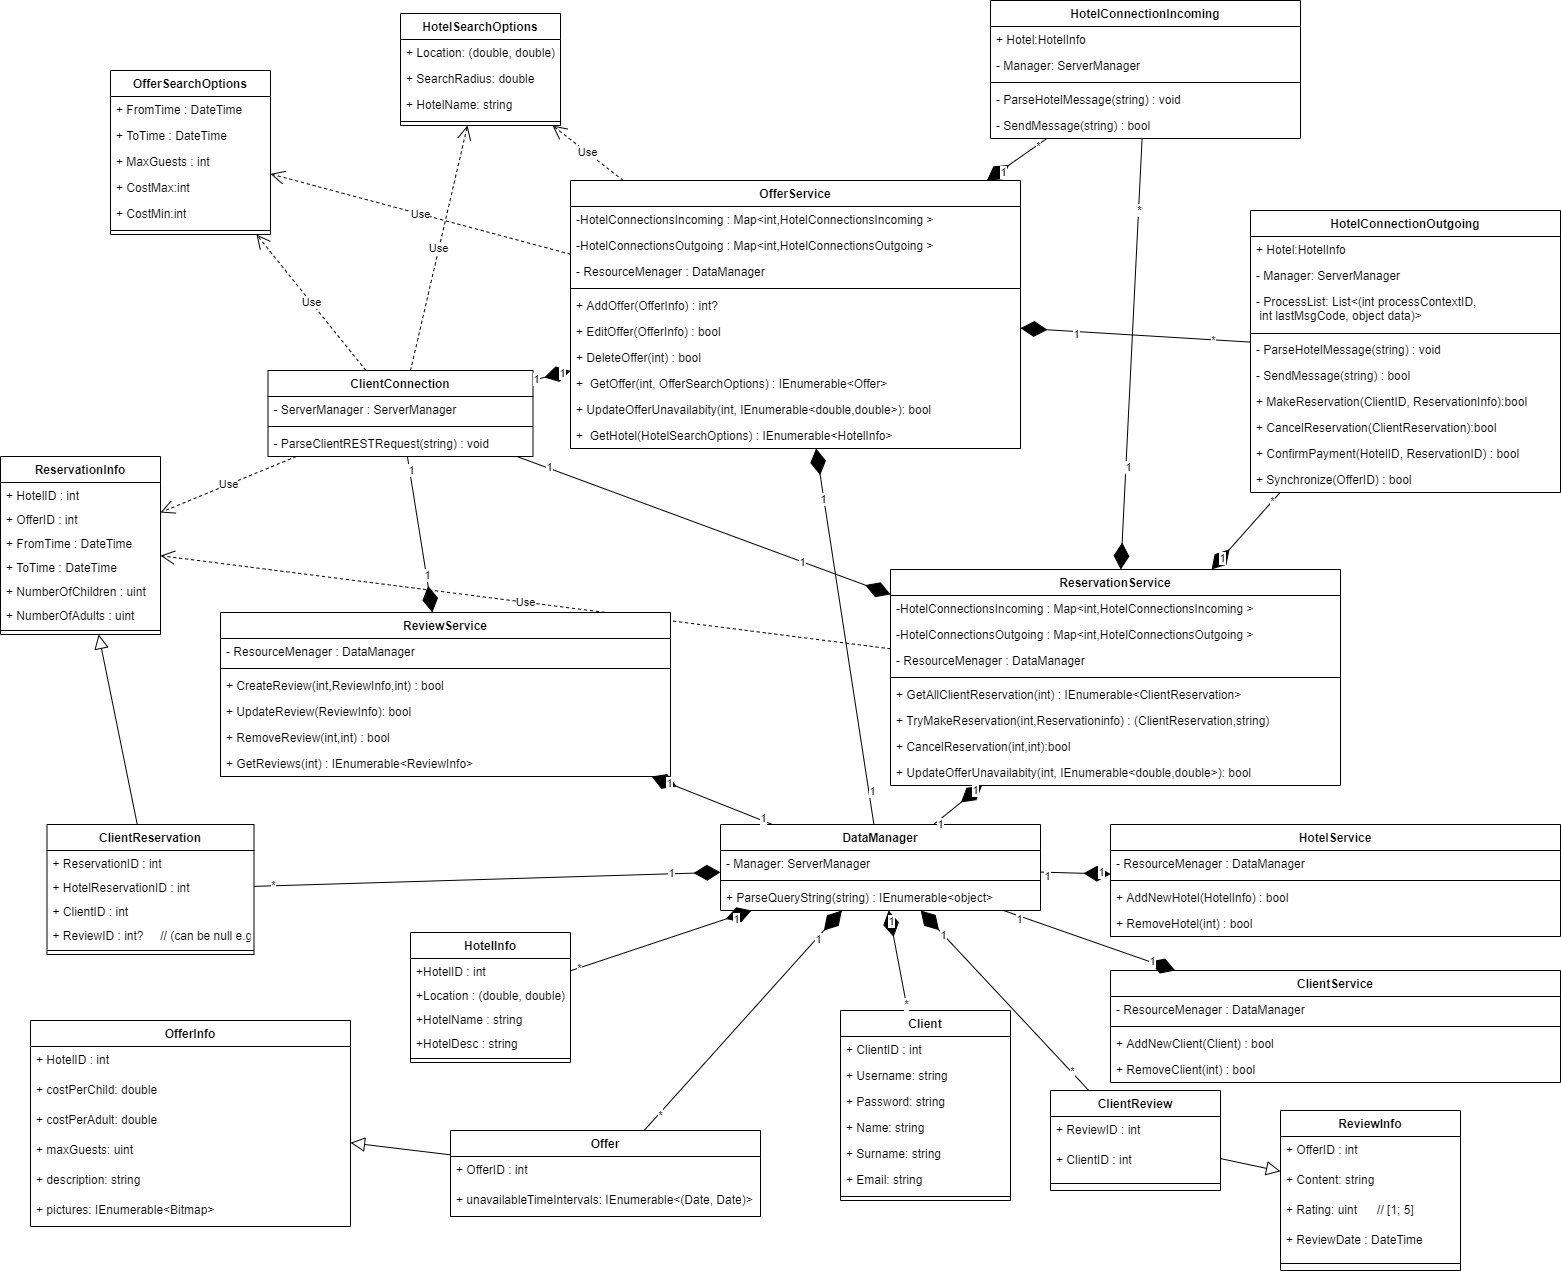
\includegraphics[scale=0.34]{checkpoint1/IO Klasy-Server_Module.png}
\end{center}

\subsubsection{Client}
Klasa trzyma informacje o kliencie.
Przedstawia jeden rekord z bazy danych.

\subsubsection{ClientConnection}
Klasa ta to interfejs sieciowy pomiędzy aplikacją kliencką i serwerem. Klasa w metodzie \texttt{ParseClientRESTRequest} implementuje procesy biznesowe związane z REST API, z których korzystają klienci. W zależności od żądania wywoływane są odpowiednie metody klasy ServerManager i zwracane są klientowi dane lub błąd (co wynika np. ze zwrócenia błędu przez odpowiednią metodę klasy ServerManager, bądź wyrzuceniem określonego typu wyjątku). Klasa ta może również przekazać żądanie do konkretnego hotelu wykorzystując metodę \texttt{GetHotelConnection} w ramach dalszej realizacji określonego procesu biznesowego (np. tworzenie rezerwacji) jednocześnie oczekując na odpowiedź od hotelu.

\subsubsection{DataManager}\label{serverModuleDataManager}
Klasa będąca interfejsem bazy danych. W serwerze jest tylko jedna instancja tej klasy, która jest używana bezpośrednio przez klasę ServerManager.

\subsubsection{HotelInfo}
Klasa trzymająca informacje o hotelach korzystających z serwisu.

\subsubsection{HotelSearchOptions}
Klasa służy do trzymania kryteriów wyszukiwania po hotelach.

\subsubsection{OfferSearchOptions}
Klasa służy do trzymania kryteriów wyszukiwania po ofertach.

\subsubsection{ReservationInfo}
Klasa zawiera informacje o pojedynczej rezerwacji bez identyfikatora tej rezerwacji.

\subsubsection{ClientReservation}
Klasa dziedziczy po ReservationInfo i ponadto łączy rezerwacje z klientem i opinią.

\subsubsection{OfferInfo}
Klasa trzymająca informacje opisowe o ofercie bez informacji o identyfikatorze oferty.

\subsubsection{Offer}
Klasa trzymająca wszystkie informacje o ofercie oraz dodatkowo informacje o przedziałach czasowych, w których oferta jest niedostępna. Informacja ta jest otrzymywana na bieżąco od hotelu w ramach procesu synchronizacji danych. ID oferty jest unikatowe w obrębie jednego hotelu (nie globalnie).

\subsubsection{ReviewInfo}
Zawiera informacje o pojedynczej opinii bez informacji o identyfikatorze opinii bądź przynależności opinii do konkretnego użytkownika.

\subsubsection{ClientReview}
Zawiera wszystkie informacje o pojedynczej opinii.

\subsubsection{Payments}
Zawiera informacje o płatnościach związanych z rezerwacjami, które nie zostały jeszcze opłacone. Klient może w dowolnym momencie pobrać informacje o nieuiszczonych płatnościach. W momencie udanej opłaty za rezerwacje usuwane są odpowiednie rekordy z tej tabeli.

\subsubsection{HotelConnectionIncoming}
Klasa stanowiąca pomost w komunikacji między hotelem oraz serwerem dla wiadomości inicjowanych przez hotel. Głównym zadaniem tej klasy jest więc interpretacja żądań formułowanych przez hotel, ich przetwarzanie i zwrócenie stosownych informacji za pomocą metody \textbf{SendMessage} czy też dalsza komunikacja z modułem serwera. 
\begin{itemize}
    \item SendMessage\\
    Podstawowy sposób wysyłania wiadomości do hotelu. Wiadomość jest przekazywana do metody jako parametr typu string. Metoda ta ma na celu zagwarantowanie poprawnego przesyłu danych (np. ponawianie prób wysyłania w przypadku chwilowego przerwania połączenia). Zwracany jest typ bool, który mówi o udanym transferze danych przez gniazdo sieciowe.
    \item ParseServerMessage\\
    W tej metodzie analizowana jest wiadomość wysłana przez hotel. Poprzez interpretację  otrzymanego kodu operacyjnego następuję rozpoznanie rodzaju żądania i jego stosowna obsługa w oparciu o przesłane parametry.  
\end{itemize}

\subsubsection{HotelConnectionOutgoing}
Klasa reprezentująca procesy biznesowe, dla których żądania wysyłane są z serwera do hotelu. Każda instancja tej klasy zawiera informacje o hotelu, w ramach którego utrzymywane jest połączenie sieciowe (pole Hotel). Ponadto zawarte jest prywatne pole ProcessList, w którym zawarte są informacje o wszystkich bieżąco realizowanych procesach biznesowych wraz z ich ID kontekstu, kodem ostatnio wysłanej wiadomości oraz danymi związanymi z ostatnio wysłaną wiadomością. Metody:
\begin{itemize}
    \item ParseHotelMessage\\
    W tej metodzie analizowana jest odpowiedź hotelu związana z danym ID kontekstu procesu. ID procesu jest wiązane z ID procesu zapisanym w polu ProcessList. W zależności od otrzymanej odpowiedzi proces może się zakończyć lub mogą zostać ponownie wywołane odpowiednie metody z klasy ServerManager, utworzona nowa wiadomość (żądanie) i kontynuacja procesu biznesowego.
    \item SendMessage\\
    Podstawowy sposób wysyłania wiadomości do hotelu. Wiadomość jest przekazywana do metody jako parametr typu string. Metoda ta ma na celu zagwarantowanie poprawnego przesyłu danych (np. ponawianie prób wysyłania w przypadku chwilowego przerwania połączenia). Zwracany jest typ bool, który mówi o udanym transferze danych przez gniazdo sieciowe.
    \item MakeReservation\\
    Metoda, która tworzy proces związany z utworzeniem nowej rezerwacji. Wysyłane jest odpowiednie żądanie do hotelu oraz odkładane jest na listę ProcessList ID nowego procesu związanego z utworzeniem nowej rezerwacji. W przypadku sukcesu tworzony jest wpis w tabeli Payments o nowo utworzonej rezerwacji, która nie jest opłacona przez klienta.
    \item CancelReservation\\
    Metoda, która tworzy proces związany z anulowaniem nowej rezerwacji. Wysyłane jest odpowiednie żądanie do hotelu oraz odkładane jest na listę ProcessList ID nowego procesu związanego z utworzeniem nowej rezerwacji. W przypadku sukcesu usuwany jest lokalny wpis o rezerwacji klienta.
    \item ConfirmPayment\\
    Metoda, która tworzy proces związany z potwierdzeniem opłaty rezerwacji. Wysyłane jest odpowiednie żądanie do hotelu oraz odkładane jest na listę ProcessList ID nowego procesu związanego z utworzeniem nowej rezerwacji. W przypadku sukcesu usuwany jest wpis o nieuiszczonej opłacie za rezerwację z tabeli Payments oraz tworzony jest wpis o nowej rezerwacji w tabeli ClientReservations.
    \item Synchronize\\
    Metoda, która tworzy proces związany z synchronizacją danych dotyczących dostępności oferty. Wysyłane jest odpowiednie żądanie do hotelu oraz odkładane jest na listę ProcessList ID nowego procesu związanego z utworzeniem nowej rezerwacji. W przypadku sukcesu aktualizowane są dane o dostępności określonej oferty za pomocą metody UpdateOfferUnavailability klasy ServerManager.
\end{itemize}

\subsubsection{ServerManager}
Klasa zawierająca wysokopoziomowe metody dostępu do bazy danych związane z określonymi procesami biznesowymi. Agreguje w sobie i udostępnia wszelkie aktywne połączenia z hotelami. Posiada również wskazanie na \textbf{DataManagera} (\ref{serverModuleDataManager}). W przypadku błędów wykonania metod zwracane mogą być błędy lub wyrzucane wyjątki, które powinny być łapane w celu określenia typu błędu. Metody: 

\begin{itemize}
    \item CreateReview, UpdateReview, RemoveReview\\
    Metody odpowiedzialne za manipulowanie opiniami znajdującymi się w bazie danych.\\
    Zwracają wartość bool określającą, czy operacja się powiodła.
    \item GetReviews\\
    Zwraca wszystkie opinie przypisane do podanej w argumencie oferty.
    \item AddOffer, EditOffer, DeleteOffer\\
    Metody odpowiedzialne za manipulowanie ofertami znajdującymi się w bazie danych.\\
    Zwracają wartość bool określającą, czy operacja się powiodła.
    \item GetOffers\\
    Zwraca wszystkie oferty spełniające podane w argumencie typu OfferSearchOptions kryteria w odniesieniu do hotelu określonego identyfikatorem przekazanym jako argument metody.
    \item GetHotels\\
    Zwraca wszystkie hotele spełniające podane w argumencie typu HotelSearchOptions kryteria.
    \item GetAllClientReservations\\
    Zwraca wszystkie rezerwacje klienta podanego w argumencie.
    \item GetHotelConnection\\
    Zwraca instancję klasy HotelConnectionOutgoing. Zwracana jest klasa reprezentująca połączenie z hotelem o identyfikatorze przekazanym jako parametr metody GetHotelConnection.
    \item TryMakeReservation\\
    Metoda próbuje stworzyć rezerwację w systemie.\\
    Zwraca instancję klasy ClientReservation i string reprezentujący identyfikator płatności za nowo utworzoną rezerwację (w przypadku sukcesu).
    \item CancelReservation\\
    Metoda usuwa rezerwację z sytemu.\\
    Zwraca wartość bool określającą, czy operacja się powiodła.
    \item ConfirmPayment\\
    Metoda mająca na celu potwierdzenie ukończenia procesu płatności przez klienta wywołując odpowiednią metodę klasy SeverConnectionOutgoing.
    \item AddNewClient\\
    Dodanie nowo zarejestrowanego użytkownika do systemu.
    \item RemoveClient\\
    Usunięcie z systemu użytkownika, który się wyrejestrował.
    \item UpdateOfferUnavailability\\
    Aktualizuje dane związane z przedziałami czasowymi niedostępności oferty w oparciu o nowo otrzymane dane z procesu synchronizacji.
\end{itemize}

\section{Diagramy stanu}
\indent \indent W tej sekcji omówione zostały stany kluczowych obiektów systemu rezerwacji pokoi hotelowych. Poniżej zamieszczone zostały diagramy UML oraz ich szczegółowe opisy.
\subsection{Pokój hotelowy}

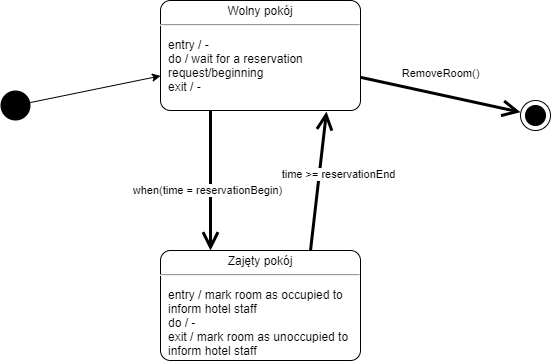
\includegraphics[width=\linewidth]{checkpoint1/RoomStateDiagram.png}
\\
\\
\indent Z każdą ofertą hotelową jest związany co najmniej jeden pokój, którego opis jest zawarty w reprezentującej go ofercie. Po utworzeniu nowego pokoju i dodaniu go do puli pokoi związanych z daną ofertą, pokój otrzymuje swój własny unikatowy identyfikator i przechodzi w stan "wolny" oczekując na rezerwację kliencką.\\
\indent W momencie rozpoczęcia rezerwacji pokój hotelowy przechodzi w stan "zajęty" - oznacza to fizyczny pobyt klienta w pokoju. Pokoje w stanie "zajętym" są wyszczególnione dla obsługi hotelowej - informacja ta może być wykorzystywana przez obsługę hotelową w celu określenia potrzeby realizacji usług takich jak regularne sprzątanie pokoju.\\
\indent W momencie zakończenia pobytu klienta w pokoju hotelowym i upływie jego rezerwacji pokój jest ponownie uwzględniany przy żądaniach rezerwacji obejmujących przedział czasowy zrealizowanej rezerwacji. Informacja o zrealizowanej rezerwacji jest usuwana w systemie hotelowym a pokój jest oznaczany jako "wolny" na okres zrealizowanej rezerwacji.\\
\indent Cykl życia obiektu pokoju hotelowego kończy się w momencie jego usunięcia z puli pokoi związanych z daną ofertą pod warunkiem, że pokój znajduje się w stanie "wolny" oraz nie są przewidziane żadne jego rezerwacje.

\subsection{Oferta pokoju}\label{offerStateDiagram}
\begin{center}
    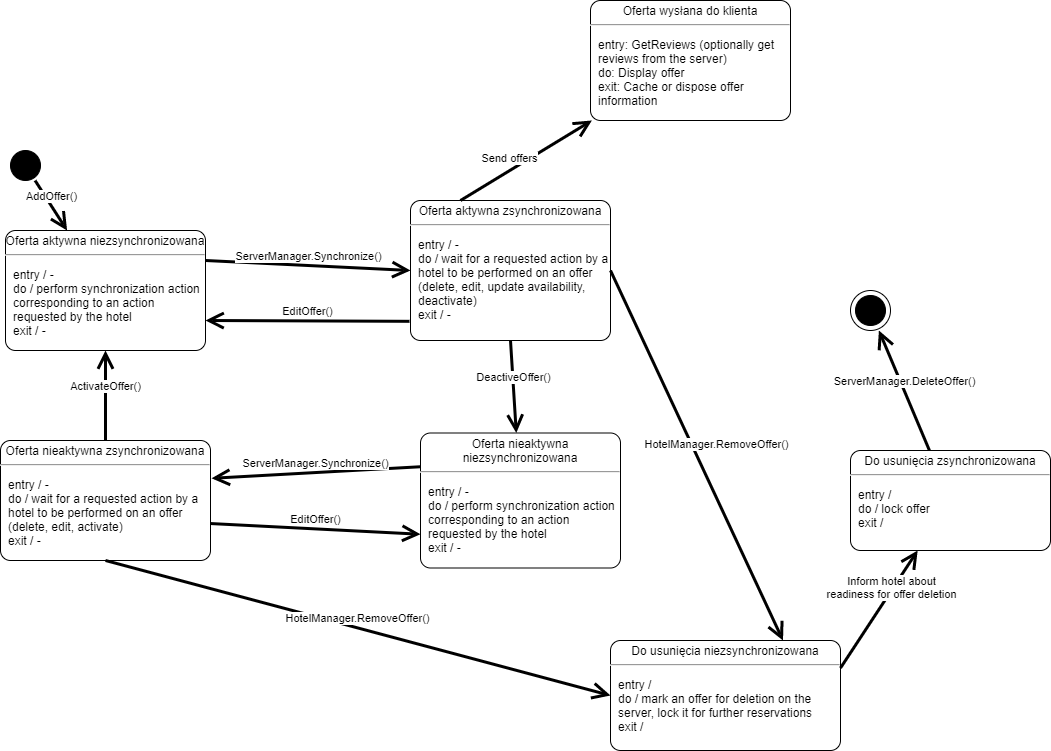
\includegraphics[scale=0.35]{checkpoint1/OfferStateDiagram.png}
\end{center}
\indent \indent Informacje o ofercie hotelowej jak i jej dostępność są przechowywane zarówno na serwerze jak i systemie hotelowym. Po utworzeniu nowej oferty w systemie hotelowym informacja o poprawnym wykonaniu tej akcji musi zostać przekazana i potwierdzona przez serwer, więc początkowym stanem nowej oferty jest "oferta aktywna niezsynchronizowana". Po poprawnej synchronizacji oferta przechodzi w stan "oferty aktywnej zsynchronizowanej".\\
\indent W przypadku edycji oferty (zmiany informacji takich jak opis pokoi, cena itp.) oferta ponownie przechodzi w stan "oferty aktywnej niezsynchronizowanej" oczekującej na wykonanie żądanych przez hotel akcji na serwerze oraz potwierdzenie ich wykonania lub informacji o błędzie. \\
\indent Oferta aktywna zsynchronizowana może zostać zdezaktywowana, dzięki czemu opcja tworzenia nowych rezerwacji jest tymczasowo niedostępna dla klientów. Oferta ta przechodzi w stan "oferty nieaktywnej niezsynchronizowanej" oczekującej na synchronizację tej akcji między modułem serwerowym i modułem hotelowym. Po pomyślnej dezaktywacji oferty przechodzi ona w stan "oferty nieaktywnej zsynchronizowanej" oczekującej na ponowną aktywację lub jej edycję przez hotel. W przypadku edycji oferta przechodzi ponownie w stan "oferty nieaktywnej niezsynchronizowanej" oczekując na zakończenie procesu syn\-chro\-nizacji serwera i hotelu, natomiast z przypadku aktywacji oferty jej stan zmienia się na "ofertę aktywną niezsynchronizowaną" oczekującą na potwierdzenie reaktywacji oferty i synchronizacji obu modułów.\\
\indent Oferty znajdujące się w stanie "aktywnym zsynchronizowanym" mogą zostać przesłane do aplikacji klienckiej w celu ich wyświetlenia. Razem z wysyłanymi ofertami mogą również zostać opcjonalnie wysłane recenzje tych ofert. Oferty te są wówczas w stanie "wysłane do klienta" a po zakończeniu ich wyświetlania obiekty reprezentujące oferty są niszczone lub zachowywane po stronie aplikacji klienckiej w celu cache'ingu.\\
\indent Oferty znajdujące się w stanie "zsynchronizowanym" mogą zostać permanentnie usunięte na żądanie systemu hotelowego. Oferta wówczas przechodzi w stan "do usunięcia niezsynchronizowana", podczas którego serwer wykonuje odpowiednie akcje związane z usunięciem oferty (oznaczenie oferty do usunięcia oraz zablokowanie możliwości tworzenia rezerwacji w ramach tej oferty) oraz informuje hotel o powodzeniu lub błędzie. W przypadku powodzenia oferta przechodzi w stan "do usunięcia zsynchronizowana" po czym obiekty reprezentujące tą ofertę są niszczone zarówno po stronie serwera jak i systemu hotelowego.

\subsection{Rezerwacja pokoju}
\begin{center}
    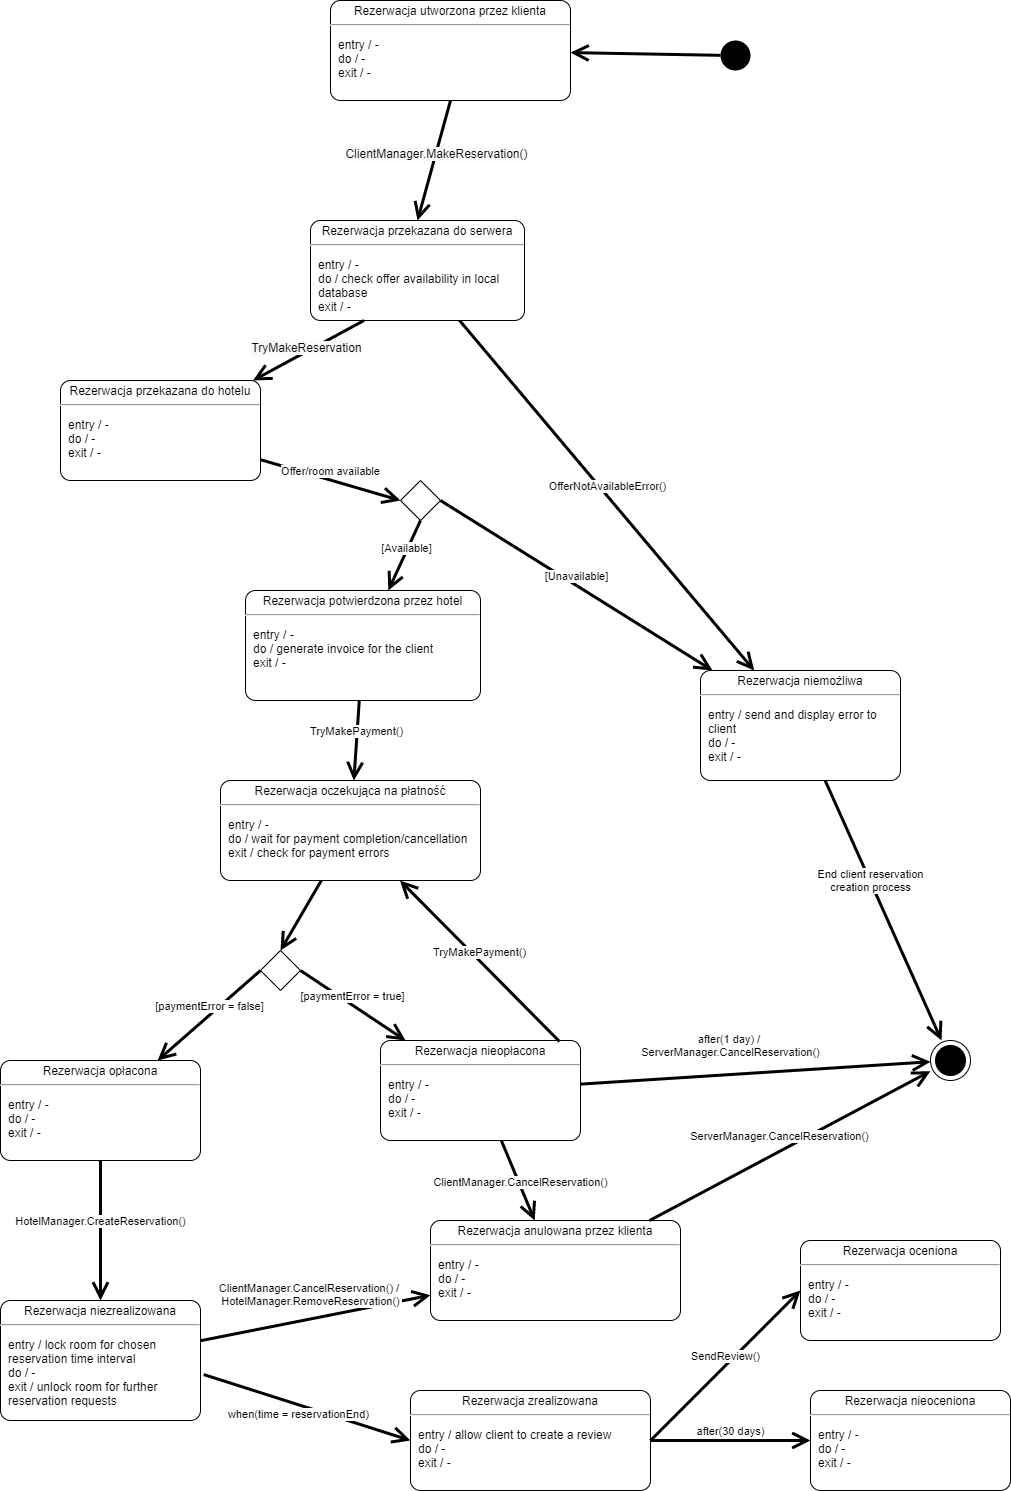
\includegraphics[scale=0.42]{checkpoint1/ReservationStateDiagram.png}
\end{center}
\indent \indent Rezerwacja pokoju hotelowego tworzona jest przez klienta w oparciu o informacje o hotelach i udostępnionych przez nie ofert jak i dostępnych terminach rezerwacji w ramach tych ofert za pomocą metody \texttt{MakeReservation}. Utworzony obiekt zawierający informacje o żądanej przez klienta rezerwacji jest w stanie "rezerwacji utworzonej przez klienta".\\
\indent Po poprawnym utworzeniu obiektu reprezentującego nową rezerwację przesyłany jest on do serwera, przechodząc w stan "rezerwacji przekazanej do serwera". Serwer w oparciu o własną lokalną bazę danych zawierającą dane związane z dostępnością ofert w określonych przedziałach czasowych (aktualizowaną na bieżąco w oparciu o komunikaty hoteli informujące o zmianie dostępności ofert) odpowiednio odrzuca żądanie rezerwacji przechodząc do stanu "rezerwacji niemożliwej" informując klienta o niedostępności oferty i ostatecznie niszcząc obiekt reprezentujący rezerwację po stronie serwera.\\
\indent W przypadku dostępności oferty w wybranym przez klienta terminie w oparciu o informacje zawarte w lokalnej bazie danych serwera żądanie rezerwacji przechodzi w stan "rezerwacji przekazy\-wanej do hotelu" w celu dodatkowej weryfikacji dostępności terminu rezerwacji po stronie systemu hotelowego. W przypadku niedostępności żadnego pokoju na określony w ramach nowej rezerwacji czas, rezerwacja przechodzi w stan "rezerwacji niemożliwej" informując klienta o błędzie oraz serwer o błędzie synchronizacji lokalnej bazy danych serwera przetrzymującej informacje o dostępności oferty z bazą danych hotelu.\\
\indent W przypadku potwierdzenia dostępności pokoju na podany przez klienta okres, oferta przechodzi do stanu "rezerwacji potwierdzonej przez hotel", podczas którego generowana jest metoda opłacenia rezerwacji przez klienta poprzez wywołanie metody \texttt{TryMakePayment}. Obiekt rezerwacji przechodzi wówczas do stanu "rezerwacji oczekującej na płatność", podczas której przeprowadzany jest proces płatności i walidacja tego procesu. W przypadku niepowodzenia rezerwacja przechodzi w stan "rezerwacji nieopłaconej". Klient może wówczas ponowić próbę płatności za rezerwację co skutkuje ponownym przejściem rezerwacji w stan "rezerwacji oczekującej na płatność".\\
\indent Możliwa jest również jawna rezygnacja klienta z rezerwacji w przypadku gdy rezerwacja jest w stanie "rezerwacji nieopłaconej" w skutek czego obiekt rezerwacji przechodzi do stanu "rezerwacji anulowanej przez klienta" i przeprowadzane są odpowiednie akcje anulowania rezerwacji po stronie klienta (\texttt{CancelReservation}). Po wywołaniu akcji \texttt{CancelReservation} po stronie serwera obiekt rezerwacji jest niszczony. W przypadku braku jawnej decyzji klienta o anulowaniu rezygnacji w momencie gdy jest ona w automatycznie anulowana po upływie 1 dnia. Po wywołaniu akcji \texttt{CancelRe\-servation} obiekt rezerwacji jest niszczony.\\
\indent W przypadku braku decyzji o anulowaniu rezerwacji oraz zakończenia procesu płatności z powo\-dzeniem rezerwacja przechodzi w stan "rezerwacji opłaconej". Po przetworzeniu zapłaty system hotelowy tworzy obiekt rezerwacji w bazie danych za pomocą metody \texttt{CreateReservation} na skutek czego rezerwacja przechodzi do stanu "rezerwacji niezrealizowanej". W przypadku anulowania rezerwacji przez klienta przyznany przez system hotelowy pokój jest zwalniany i ponownie uwzględniany w kolejnych żądaniach rezerwacji. Anulowana rezerwacja przechodzi wówczas do stanu "rezerwacji anulowanej przez klienta".\\
\indent Po upływie czasu rezerwacji obiekt przechodzi w stan "rezerwacji zrealizowanej", natomiast zarezerwowany pokój jest ponownie uwzględniany w nowych żądaniach rezerwacji. Przed upływem 30 dni klient może wystawić opinię oferty, w ramach zrealizowanej rezerwacji pokoju hotelowego. Zapisywana jest wówczas recenzja klienta, natomiast obiekt rezerwacji przechodzi wówczas do stanu "rezerwacji ocenionej".

\section{Diagramy aktywności i sekwencji}
Poniżej prezentujemy diagramy sekwencji przedstawiające przebieg komunikacji pomiędzy modułami przy realizacji najistotniejszych naszym zdaniem funkcjonalności systemu. Uwzględnione są również błędy czy alternatywne przebiegi komunikacji. Na diagramach wyróżnieni są następujący aktorzy: system hotelowy (moduł hotelowy), serwer (moduł serwera), aplikacja kliencka/ClientApp (moduł klienta). W celu zwiększenia czytelności diagramów ignorowane są błędy wynikające z utraty czy braku połączenia. 
\subsection{Oferta}
Jedną z najważniejszych funkcjonalności naszej aplikacji jest możliwość dynamicznego zarządzania ofertami przez managera hotelu (zarządcy modułu hotelowego). Dla każdej oferty można, więc przeprowadzić następujące operacje:
\begin{itemize}
    \item Dodawanie nowej oferty do systemu
    \item Usuwanie już istniejącej oferty - jeśli oferta z jakichkolwiek powodów przestanie być aktualna (zakończenie okresu promocji, wyczerpanie liczby dostępnych ofert) udostępniamy możliwość trwałego usunięcia jej z systemu, tak aby przestała być widoczna dla klientów
    \item Edytowanie oferty - w przypadku zaistnienia konieczności modyfikacji już istniejącej oferty manager ma możliwość zmiany dowolnego parametru oferty. W tym celu posługuje się dobrze mu znanym formularzem dodawania nowej oferty z naniesioną bieżącą postacią oferty.  
\end{itemize}
Przebieg komunikacji dla każdej z tych operacji prezentujemy poniżej.
\subsubsection{Dodawanie oferty}
\begin{center}
    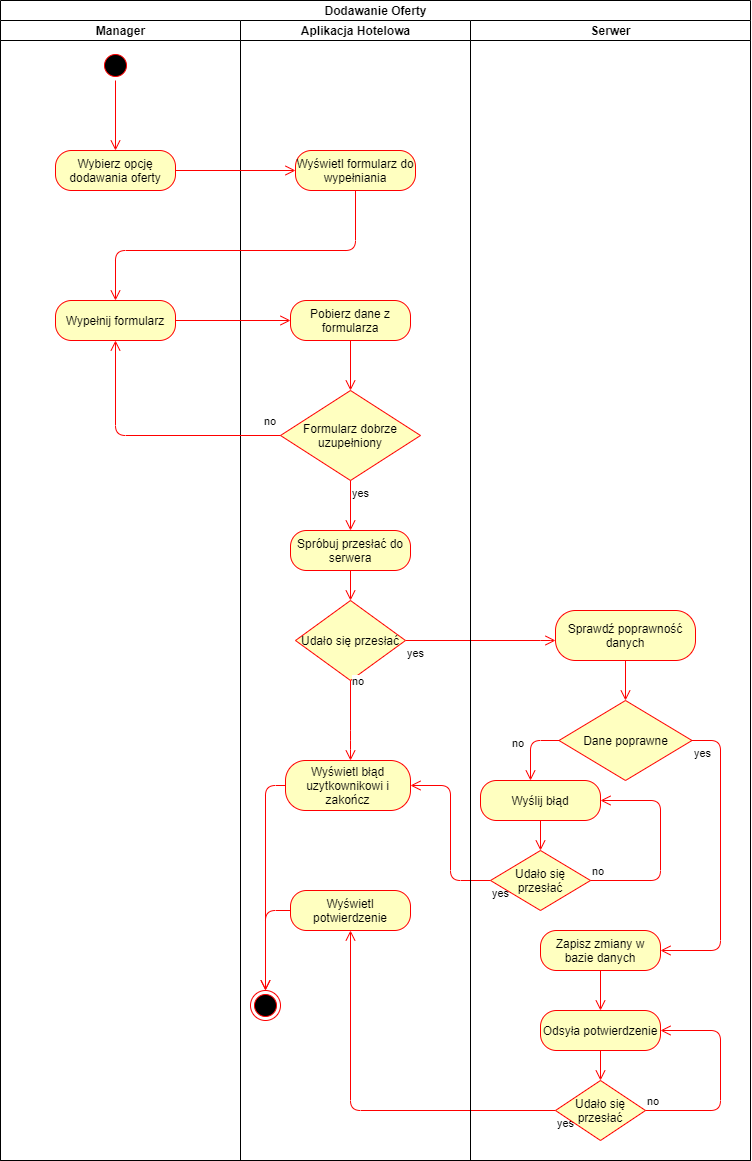
\includegraphics[scale=0.4]{Aktywnosc/IO_Aktywności-Dodawanie oferty.png}\newpage
    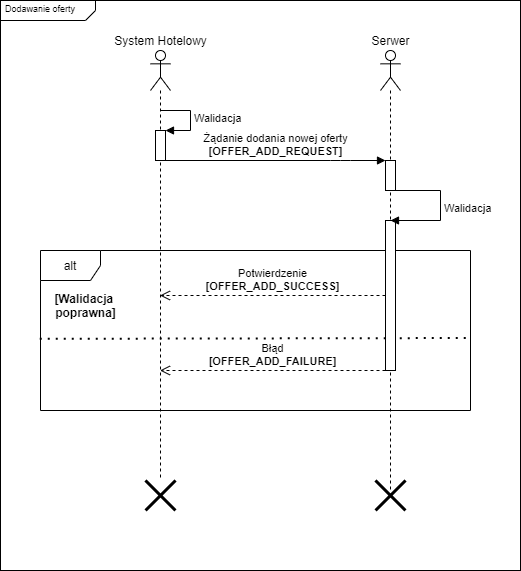
\includegraphics[width=\linewidth]{Sekwencje/Offer_Add.png}
\end{center}
Dodawanie oferty to operacja między Systemem Hotelowym, a Serwerem.
System Hotelowy wysyła po walidacji lokalnej żądanie do serwera wraz z wszystkimi informacjami o ofercie.
Serwer po otrzymaniu żądania waliduje otrzymane dane po czym odsyła serwerowi czy operacja się powiodła, wtedy odsyła potwierdzenie, czy nastąpił jakiś błąd, wtedy odsyła informacje o błędzie.
Jeśli system hotelowy nie może wysłać komunikatu ponawia próbę po pewnym czasie. Powtarza to 5 razy co sekundę, po czym zarzuca wykonywanie aktywności.
W przypadku otrzymania potwierdzenia System Hotelowy kończy operacje dodaniem do swojej bazy danych oferty.
W przypadku niepowodzenia oferta nie zostaje dodana do bazy danych i proces się kończy.
\subsubsection{Usuwanie oferty}
\begin{center}
    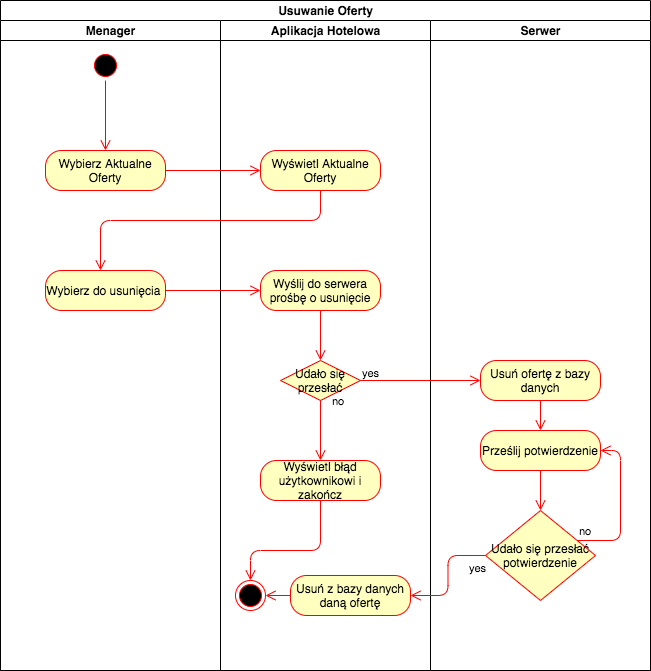
\includegraphics[scale=0.5]{Aktywnosc/IO_Aktywności-Usuwanie oferty.png}
    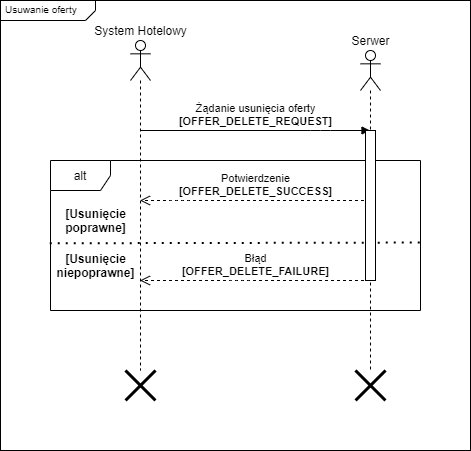
\includegraphics[scale=0.65]{Sekwencje/Offer_Delete.png}
\end{center}

Usuwanie oferty odbywa się w następujący sposób System hotelowy wysyła żądanie, a Serwer odsyła informacje o powodzeniu operacji lub o błędzie.
Jeśli system hotelowy nie może wysłać komunikatu ponawia próbę po pewnym czasie. Powtarza to 5 razy co sekundę, po czym zarzuca wykonywanie aktywności.
\subsubsection{Edytowanie oferty}
\begin{center}
    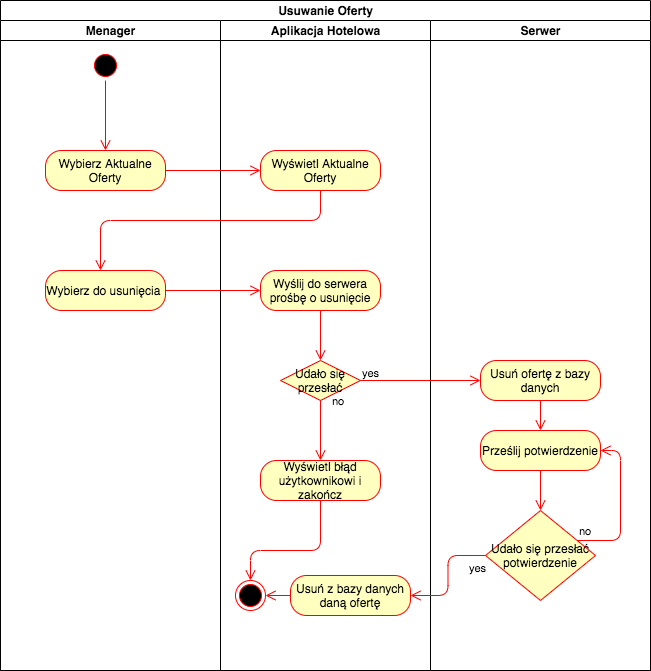
\includegraphics[scale=0.4]{Aktywnosc/IO_Aktywności-Usuwanie oferty.png}
    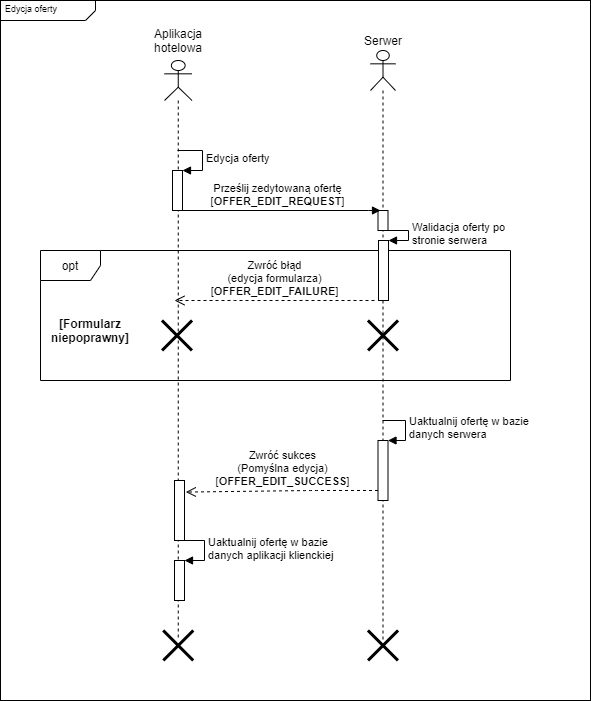
\includegraphics[scale=0.4]{Sekwencje/Offer_Edit.png}
\end{center}

Edycja oferty zaczyna się od wypełnienia formularza zmian przez użytkownika Systemu Hotelowego wewnątrz niej. Zmiany są następnie wstępnie walidowane. W przypadku nieudanej walidacji użytkownik jest z powrotem odsyłany do formularza. W przypadku udanej walidacji System Hotelowy wysyła żądanie wprowadzenia zmian do Serwera który jeszcze raz waliduje otrzymane dane. Jeśli to się nie powiedzie odsyła błąd i proces się kończy. W przypadku przejścia walidacji pomyślnie system uaktualnia dane i odsyła informacje o powodzeniu operacji po czym System Hotelowy uaktualnia swoje dane.
Jeśli system hotelowy nie może wysłać komunikatu ponawia próbę po pewnym czasie. Powtarza to 5 razy co sekundę, po czym zarzuca wykonywanie aktywności.
\subsubsection{Wyszukiwanie oferty}
\begin{center}
    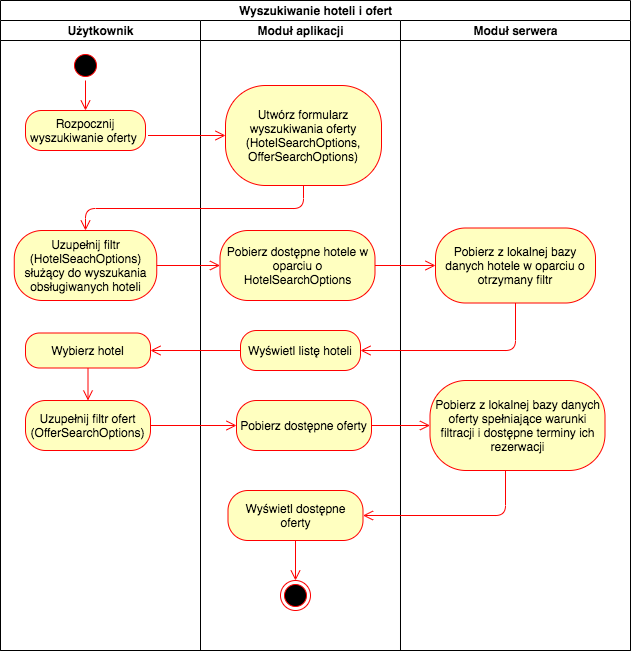
\includegraphics[scale=0.65]{Aktywnosc/IO_Aktywności-Wyszukiwanie hoteli i ofert.png} \newpage
    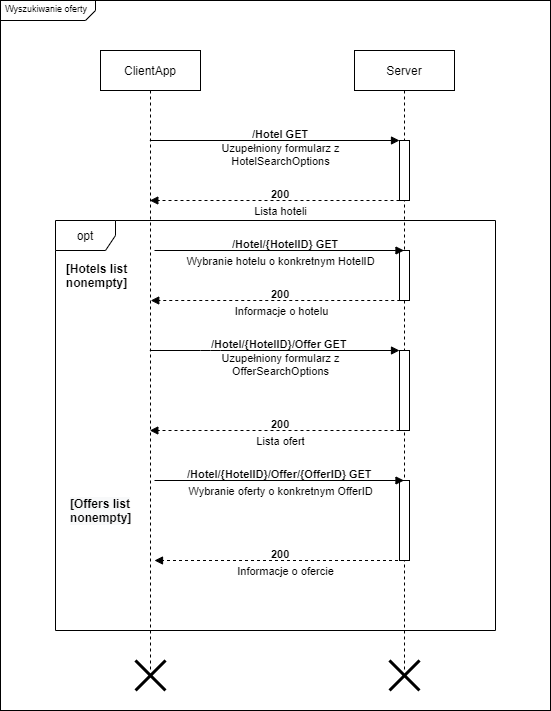
\includegraphics[scale=0.65]{Sekwencje/Offer_Search.png}
\end{center}

Wyszukiwanie oferty w systemie jest 2 etapowe.\newline
Pierwszy etap to uzupełnienie danych wyszukiwania hotelu. Wypełniony formularz jest przesyłany do serwera. Tam odbywa się jego walidacja. W przypadku nieprawidłowości w formularzu do użytkownika zostaje przesłany błąd w postaci kodu 400 wraz z informacją o błędnie wypełnionym polu. Jeśli formularz został wypełniony poprawnie zwracana jest lista hoteli. W przypadku gdy lista jest niepusta możemy wybrać jeden z hoteli, aby poznać szczegółowe informacje na jego temat i mieć dostęp do udostępnionych przez niego ofert.\\ 
Drugi etap to wyszukiwanie ofert spośród tych udostępnionych przez wybrany we wcześniejszych krokach hotel. Wyszukiwanie to przebiega analogicznie do wyszukiwania hoteli. Użytkownik ma możliwość ograniczenia listy ofert poprzez wypełnienie danych do wyszukiwania ofert. Formularz jest przesyłany do serwera gdzie odbywa się jego walidacja. W przypadku nieprawidłowości do użytkownika zostaje przesłany błąd w postaci kodu 400 wraz z informacją o błędnie wypełnionym polu.
Jeśli formularz został wypełniony poprawnie zwracana jest lista ofert. W przypadku gdy lista jest niepusta możemy wybrać jedną z ofert, aby poznać jej szczegóły i przejść do dalszej interakcji.\\
Jeśli system hotelowy nie może wysłać komunikatu ponawia próbę po pewnym czasie. Powtarza to 5 razy co sekundę, po czym zarzuca wykonywanie aktywności.\\
Walidacja formularza i ewentualnie zwracane błędy w postaci kodów 400 nie zostały naniesione na diagram w celu zachowania jego czytelności. 

\subsection{Rezerwacja}
Podstawą systemu jest możliwość składania rezerwacji przez klientów. W poniższej podsekcji zobaczymy jak wygląda z grubsza komunikacja między modułami podczas tworzenia i anulowania rezerwacji przez klienta.
\subsubsection{Tworzenie rezerwacji} \label{reservation_diagram}
\begin{center}
    \includegraphics[scale=0.237]{Aktywnosc/IO_Aktywności-Tworzenie rezerwacji.png}
\end{center}
\begin{center}
    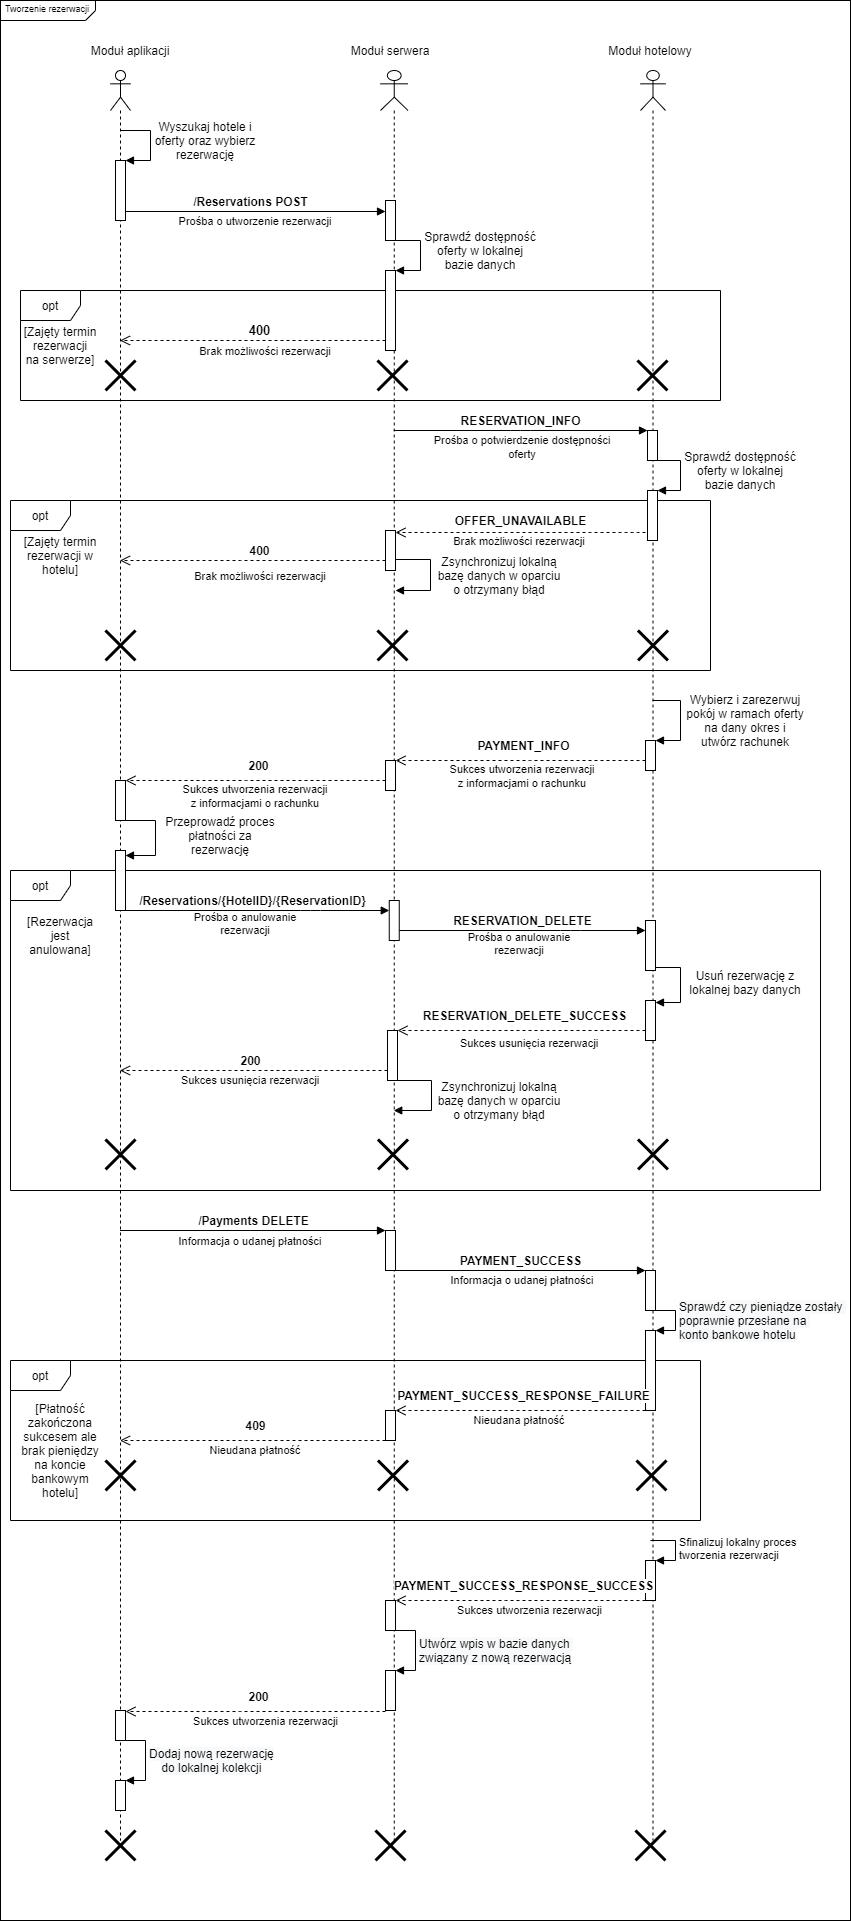
\includegraphics[scale=0.3]{Sekwencje/Reservation_Create.png}
\end{center}
\indent \indent Proces tworzenia rezerwacji zaczyna się po wybraniu przez użytkownika aplikacji klienckiej hotelu oraz oferty, w ramach której ma być utworzona nowa rezerwacja. Prośba o utworzenie nowej rezerwacji jest przesyłana do serwera, który sprawdza czy oferta jest dostępna w oparciu o własne dane uzyskane z hotelu. W przypadku braku wolnego terminu zwracany jest błąd i kończony jest proces tworzenia rezerwacji. 
\newline
\indent Jeśli jednak z lokalnych danych wynika możliwość utworzenia rezerwacji, przesyłane jest żądanie do hotelu o wstępne utworzenie rezerwacji. Hotel w oparciu o swoje dane ponownie sprawdza dostępność oferty. W przypadku gdy oferta nie jest dostępna w wyznaczonym czasie zawracany jest błąd, który oznacza desynchronizację między danymi hotelu a serwera opasującymi dostępność oferty. W efekcie serwer odsyła użytkownikowi informację o nieudanej rezerwacji oraz natychmiastowo wykonuje proces związany z synchronizacją danych. 
\newline
\indent W przypadku gdy hotel będzie mógł przyporządkować odpowiedni pokój na podany okres czasowy, tworzy on lokalny wpis w bazie danych związany z tą rezerwacją oraz wpis dotyczący płatności za tą rezerwację, która musi zostać opłacona przez klienta, a następnie wysyłana do klienta przez serwer.
\newline
\indent Klient może anulować rezerwację oraz wysłać do serwera odpowiedni komunikat, który następnie jest przesyłany do hotelu. Hotel usuwa wówczas utworzony wpis rezerwacji i zwraca odpowiednią informację serwerowi, która jest propagowana do klienta.
\newline
\indent Jeśli klient opłaci w czasie daną rezerwację, wysyłany jest komunikat do serwera o zakończeniu procesu płatności, który jest następnie przekazywany do hotelu. Hotel ponownie sprawdza czy płatność związana z konkretnym identyfikatorem płatności została zakończona sukcesem.
\newline
\indent W przypadku niepowodzenia zwracana jest wiadomość do serwera oznaczająca konieczność kontaktu z hotelem w celu potwierdzenia płatności. Jest to sytuacja szczególna, która może być zależna od zewnętrznego dostawcy usług płatności i błędami w tym systemie płatności lub brakiem odpowiedniej synchronizacji (ten przypadek szczególny został opisany przy (\ref{payments})).
\newline
\indent Jeśli płatność zostanie potwierdzona przez hotel, jest odsyłana odpowiedź o sukcesie do serwera, w wyniku czego tworzony jest wpis o rezerwacji klienckiej po stronie serwera i odsyłana odpowiednia odpowiedź stanowiąca o sukcesie całego procesu rezerwacji.

\subsubsection{Anulowanie rezerwacji}
\begin{center}
    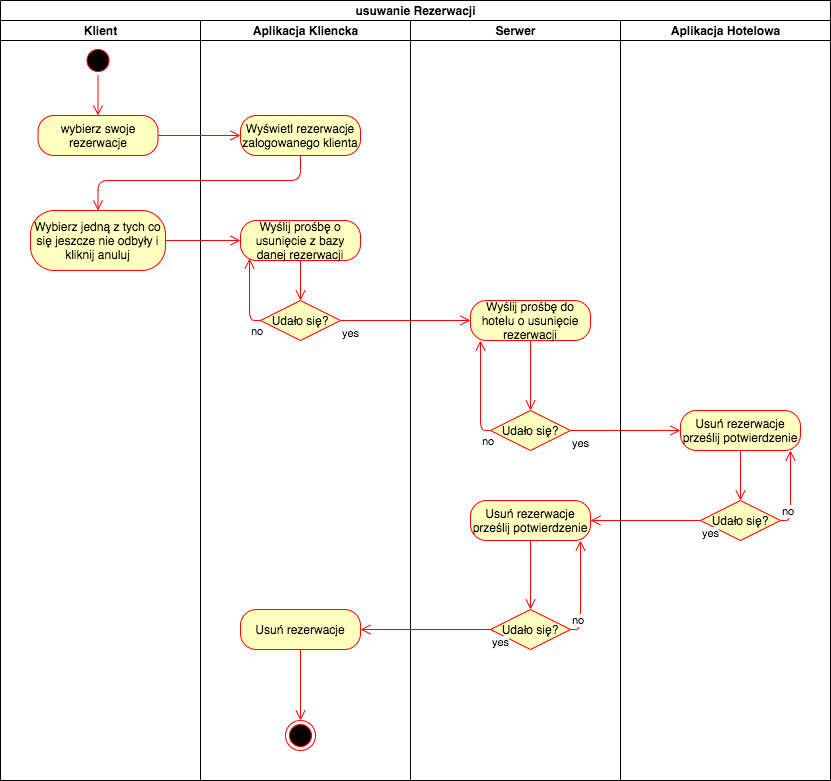
\includegraphics[scale=0.4]{Aktywnosc/IO_Aktywności-Usuwanie rezerwacji.png}\newpage
    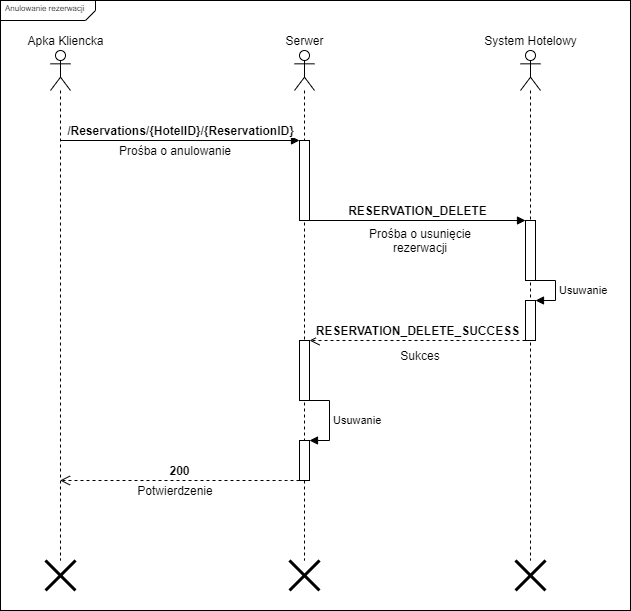
\includegraphics[width=\linewidth]{Sekwencje/Reservation_Cancel.png}
\end{center}

Po wybraniu swojej rezerwacji klient ma możliwość anulowania jej. Aplikacja Kliencka wysyła wtedy żądanie usunięcia rezerwacji do Serwera który przekazuje ją odpowiedniemu hotelowi. Hotel usuwa ze swojej bazy danych rezerwacje i przesyła potwierdzenie do Serwera który również usuwa rezerwację z swojej bazy danych i przesyła potwierdzenie do klienta. W przypadku wystąpienia błędu na którymkolwiek z tych etapów przesyłany jest błąd w stronę klienta i żadne zmiany w bazie danych nie są robione.
Jeśli któryś z modułów nie może wysłać komunikatu ponawia próbę po pewnym czasie. Powtarza to 5 razy co sekundę, po czym zarzuca wykonywanie aktywności.
\subsubsection{Tworzenie rezerwacji lokalnie}
\begin{center}
    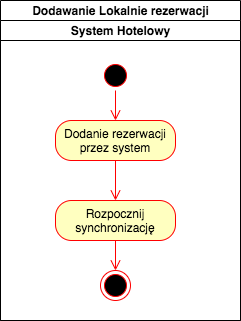
\includegraphics[scale=1]{Aktywnosc/IO_Aktywności-Local reservation.png}
\end{center}
Istnieje również możliwość że klient przyjdzie do hotelu bez rezerwacji. System hotelowy ma możliwość właśnie na taką ewentualność. System hotelowy może zarezerwować pokój w imieniu klienta Po takiej rezerwacji nie może zostać strwożona opinia gdyż serwer nie wie o istnieniu takowej. Id klienta w bazie danych systemu hotelowego jest IdUser hotelu. Hotel nie przetrzymuje wtedy żadnych informacji o kliencie, ale za to klient nie musi trwożyć nowego konta. System Hotelowy próbuje synchronizować się z serwerem i gdy nie ma żadnych przeciwności(czytaj np. nie ma rezerwacji które były na serwerze na dany okres, a system hotelowy o nich nie wiedział) dodaje rezerwację do lokalnej bazy danych.
\subsection{Opinia}
W celu umożliwienia oceny danej oferty klienci(użytkownicy aplikacji klienckiej) mają możliwość dodawania swoich opinii do ofert z których ostatnio skorzystali. Poniżej przedstawiamy proces dodawania takiej opini do systemu.
\subsubsection{Dodawanie opinii}
\begin{center}
    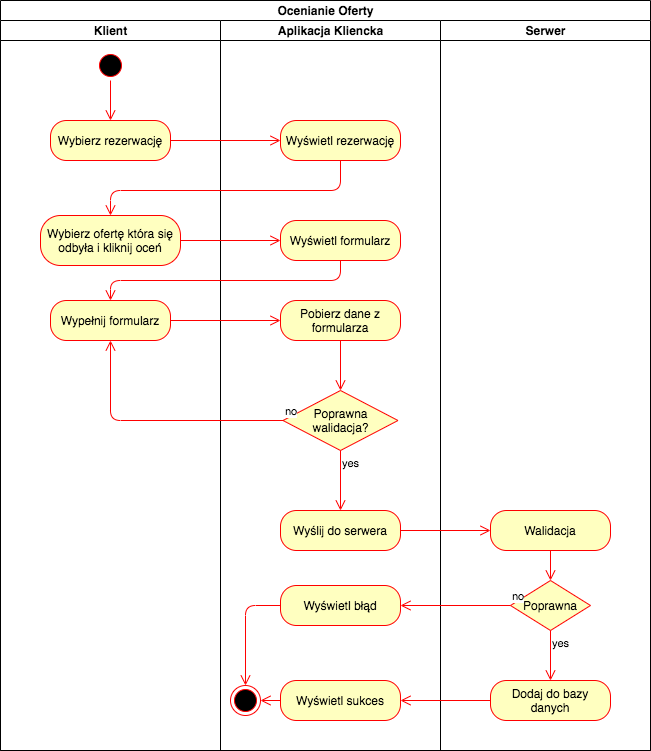
\includegraphics[width=\linewidth]{Aktywnosc/IO_Aktywności-Dodawanie oceny.png}\newpage
    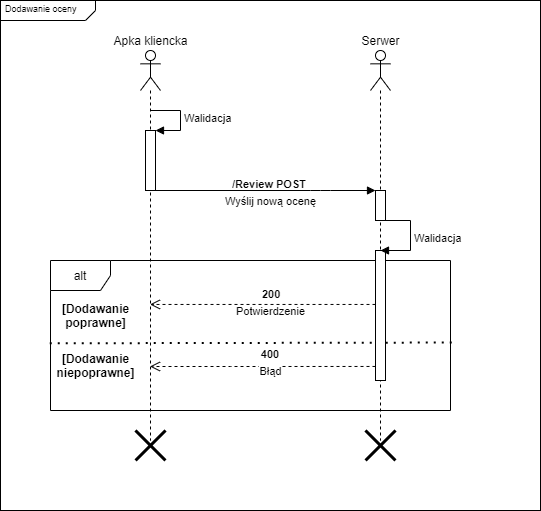
\includegraphics[width=\linewidth]{Sekwencje/Opinion_Add.png}
\end{center}

Klient może dodać opinie do wybranej przez siebie rezerwacji którą już odbył. W tym celu wypełnia formularz w Aplikacji Klienckiej, który jest walidowany (w przypadku niepowodzenie odsyłany jest z powrotem do formularza). Po przejściu przez walidację żądanie wysyłane jest do Serwera który ponownie je waliduje i odsyła informacje czy operacja się powiodła czy nie.
\subsection{Synchronizacja}
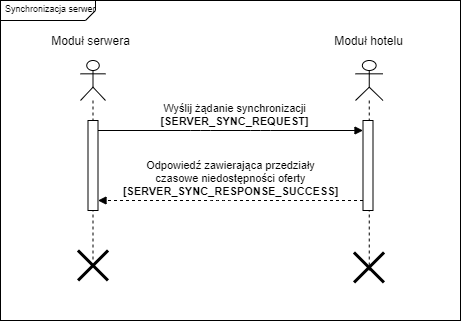
\includegraphics[width=\linewidth]{Sekwencje/Synchronization_Server.png.png}
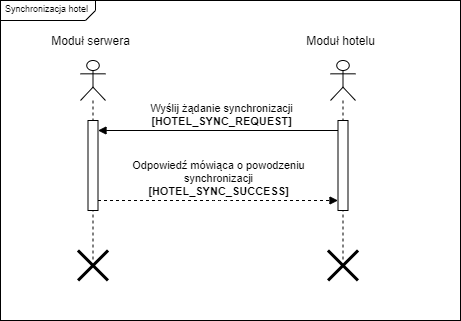
\includegraphics[width=\linewidth]{Sekwencje/Synchronization_Hotel.png}
W dowolnym momencie dane między hotelem a serwerem dotyczące dostępności ofert mogą się zdesynchronizować. Może to wynikać np. z błędów systemowych/sprzętowych po stronie serwera powodujących utratę danych, przeorganizowanie przyporządkowań pokoi do rezerwacji czy utworzenia nowej, anonimowej rezerwacji w hotelu niezależnej od systemu. W celu zsynchronizowania danych, zarówno serwer jak i hotel mogą rozpocząć procedurę synchronizacji danych w odniesieniu do konkretnej oferty hotelowej. Przesyłane są wówczas dane zawierające przedziały czasowe niedostępności ofert odpowiednio wyznaczone przez hotel.


\section{Hotel-Serwer}
Do przesyłania wiadomości używane są trwałe połączenia TCP. Wynika to z faktu, że komunikacja między modułami hotelowymi a modułem serwerowym może się rozpocząć zarówno po stronie hotelu jak i serwera. Format przesyłanych wiadomości jest następujący:
\begin{enumerate}
    \item Unsigned integer (enum) oznaczający kontekst wiadomości (kod operacyjny)
    \item Unsigned integer oznaczający id kontekstu (procesu) pozwalający odróżnić wiadomość od innych o takim samym kodzie operacyjnym (w przypadku gdy realizowanych jest kilka takich samych procesów biznesowych jak tworzenie rezerwacji, istnieje konieczność odróżnienia, który ciąg wiadomości odnosi się do którego procesu)
    \item Unsigned integer oznaczający liczbę bajtów przesyłanych danych
    \item Ciąg bajtów danych zawierający zserializowany obiekt JSON
\end{enumerate}
Standard unsigned integerów to ISO/IEC 9899. Standardem zapisu JSONa jest UTF-8. Pozwoli nam to zachować polskie znaki wewnątrz Opinii klientów i wewnątrz Ofert wystawianych przez Hotele.
W odniesieniu do jednego połączenia TCP między hotelem oraz serwerem procesy biznesowe i wiadomości są podzielone na 2 grupy - procesy, których żądania związane z rozpoczęciem są zawsze żądaniami wychodzącymi oraz procesy, których żądania związane z rozpoczęciem tego procesu są zawsze żądaniami przychodzącymi. Każdy z tych procesów jest związany z oddzielnym gniazdem sieciowym realizującym połączenie TCP (te same adresy IP, ale różne porty). Każda z tych grup może być przetwarzana przez oddzielny proces na danym module (zatem w ramach jednego połączenia wyróżniamy 4 procesy: 2 procesy po stronie serwera przetwarzające procesy związane z żądaniami wychodzącymi (serwera) i przychodzącymi (hotelu) oraz 2 procesy po stronie hotelu przetwarzające procesy związane z żądaniami przychodzącymi (serwera) i wychodzącymi (hotelu)). Procesy te w obrębie jednego modułu są od siebie niezależne, wykorzystując własne gniazda sieciowe oraz mogą przetwarzać wiele procesów jednocześnie przyporzą\-dkowując odpowiednie id kontekstu procesu w wysyłanych wiadomościach.
W przypadku źle sformatowanej wiadomości nie robimy nic.

Poniżej zostały przedstawione wszystkie kody operacyjne wraz z ich prawdziwymi wartościami.
\begin{center}
    \begin{tabular}{|c|c|c|}\hline
        kod operacyjny & numer & wysyłany przez\\ \hline \hline
        HOTEL\_LOGIN\_REQUEST & 1 & Hotel\\ \hline
        HOTEL\_LOGIN\_RESPONSE\_SUCCESS & 2 & Serwer\\ \hline
        HOTEL\_LOGIN\_RESPONSE\_FAILURE & 3 & Serwer\\ \hline
        HOTEL\_SYNC\_REQUEST & 4 & Hotel\\ \hline
        HOTEL\_SYNC\_RESPONSE\_SUCCESS & 5 & Serwer\\ \hline
        SERWER\_SYNC\_REQUEST & 6 & Serwer\\ \hline
        SERWER\_SYNC\_RESPONSE\_SUCCESS & 7 & Hotel\\ \hline
        RESERVATION\_CREATE & 8 & Serwer\\ \hline
        RESERVATION\_GET & 9 & Serwer\\ \hline
        RESERVATION\_GET\_RESPONSE & 10 & Hotel\\ \hline
        OFFER\_UNAVALAIBLE & 11 & Hotel\\ \hline
        PAYMENT\_INFO & 12 & Hotel\\ \hline
        PAYMENT\_SUCCESS & 13 & Serwer\\ \hline
        PAYMENT\_SUCCESS\_RESPONSE\_SUCCESS & 14 & Hotel\\ \hline
        PAYMENT\_SUCCESS\_RESPONSE\_FAILURE & 15 & Hotel\\ \hline
        ID\_UNKNOWN & 16 & Hotel\\ \hline
        RESERVATION\_DELETE & 17 & Serwer\\ \hline
        RESERVATION\_DELETE\_SUCCESS & 18 & Hotel\\ \hline
        RESERVATION\_DELETE\_FAILURE & 19 & Hotel\\ \hline
        OFFER\_ADD\_REQUEST & 20 & Hotel\\ \hline
        OFFER\_ADD\_SUCCESS & 21 & Serwer\\ \hline 
        OFFER\_ADD\_FAILURE & 22 & Serwer\\ \hline
        OFFER\_DELETE\_REQUEST & 23 & Hotel\\ \hline
        OFFER\_DELETE\_SUCCESS & 24 & Serwer\\ \hline 
        OFFER\_DELETE\_FAILURE & 25 & Serwer\\ \hline   
        OFFER\_EDIT\_REQUEST & 26 & Hotel\\ \hline
        OFFER\_EDIT\_SUCCESS & 27 & Serwer\\ \hline 
        OFFER\_EDIT\_FAILURE & 28 & Serwer\\ \hline
    \end{tabular}
\end{center}

\subsection{Logowanie i uwierzytelnienie hotelu}

\subsubsection{\texttt{HOTEL\_LOGIN\_REQUEST}}
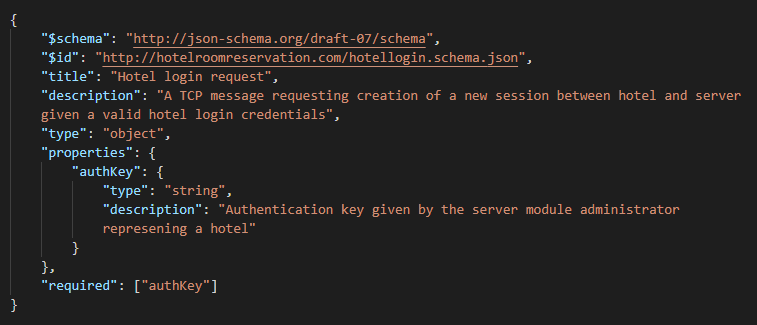
\includegraphics[width=\linewidth]{Hotel login + synchronizacja/hotel_login_request.png}
\indent W celu możliwości zarządzania ofertami hotelowymi i tworzenia rezerwacji system hotelowy musi nawiązać trwałe połączenie TCP z serwerem. Po nawiązaniu połączenia na znany adres IP i numer portu serwera pierwszym komunikatem wysyłanym przez hotel musi być wiadomość o kodzie operacyjnym \texttt{HOTEL\_LOGIN\_REQUEST} oraz zserializowanym obiektem JSON zgodnym ze schematem załączonym powyżej. W obiekcie tym znajduje się właściwość “authKey” będąca kluczem autentykacyjnym hotelu. Unikatowe klucze autentykacyjne są uprzednio nadawane przez administratora serwera każdemu hotelowi korzystającemu z serwisu. W związku z faktem, że połączenie składa się z 2 gniazd sieciowych przetwarzających różne grupy procesów biznesowych powyższa wiadomość musi być przesłana do każdego gniazda oddzielnie po nawiązaniu połączenia.

Do kodów “akceptowalnych” należą:
\begin{itemize}
    \item \texttt{HOTEL\_LOGIN\_RESPONSE\_SUCCESS} - wiadomość mówiąca o udanym zalogowaniu. Utworzone zostaje stałe łącze TCP między hotelem a serwerem, przez które mogą być wysyłane nowe żądania. Wiadomość ta składa się jedynie z kodu operacyjnego - nie jest przesyłany zserializowany obiekt JSON.
    \item \texttt{HOTEL\_LOGIN\_RESPONSE\_FAILURE}
\end{itemize}

\subsubsection{\texttt{HOTEL\_LOGIN\_RESPONSE\_FAILURE}}
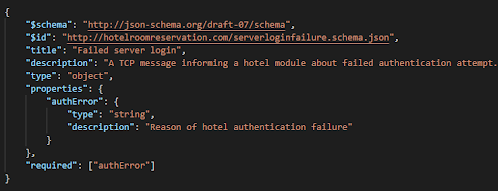
\includegraphics[width=\linewidth]{Hotel login + synchronizacja/hotel_login_response_failure.png}
\indent Wiadomość wysyłana w przypadku niepowodzenia procesu logowania hotelu do serwisu. Zawiera ona obiekt JSON z właściwością “authError” zawierającą szczegółowy opis błędu autentykacji.

\subsection{Synchronizacja}
\indent \indent Informacje o rezerwacji są przechowywane zarówno w bazie danych modułu hotelowego jak i modułu serwera. Gdy klient wyszukuje oferty możliwych do rezerwacji w określonym zakresie czasowym serwer znajduje odpowiadające oferty w oparciu o własne dane dotyczące przedziałów czasowych, w których dana oferta jest niedostępna. Dane te są na bieżąco aktualizowane z hotelami podczas procesu tworzenia i anulowania rezerwacji jak i w ramach możliwego mechanizmu periodycznej synchronizacji obu modułów. W przypadku gdy zostanie utworzona nowa rezerwacja anonimowa (na miejscu w hotelu) bądź system hotelowy przeorganizuje dopasowanie pokoi do rezerwacji tworząc lub zamykając tym samym “okna” dostępności danej oferty potrzebna jest synchronizacja danych dostępności danej oferty z serwerem. Ponadto, system synchronizacji jest częścią procesu anulowania jak i tworzenia rezerwacji po stronie serwera. Serwer może w nieoczekiwanym przypadku mieć nieaktualne dane związane z dostępnością oferty w momencie wysłania wiadomości do hotelu o utworzeniu nowej rezerwacji. W efekcie zostanie zwrócony błąd o niedostępności oferty, przez co serwer zmuszony będzie do niezwłocznego wysłania żądania o synchronizacje danych.

\subsubsection{\texttt{HOTEL\_SYNC\_REQUEST}}
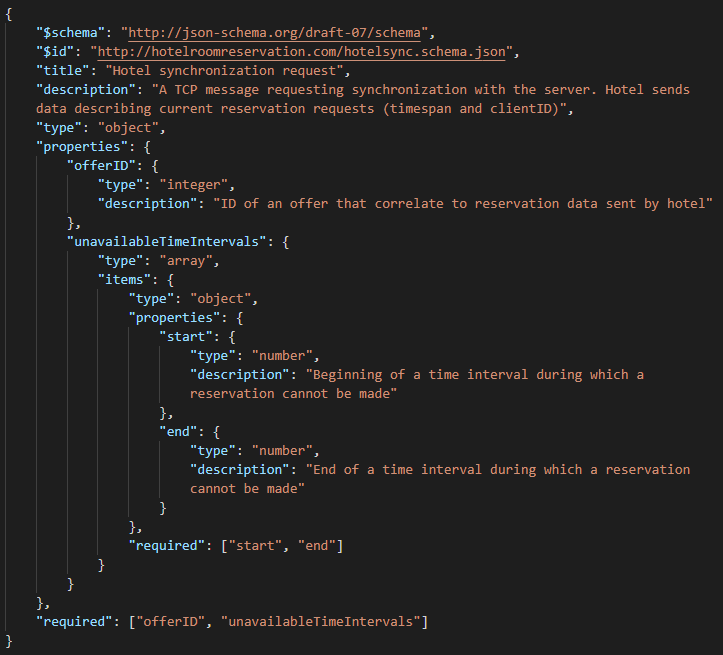
\includegraphics[width=\linewidth]{Hotel login + synchronizacja/hotel_sync_request.png}
\indent Wiadomość ta jest żądaniem synchronizacji danych dotyczących dostępności oferty wysyłanym przez hotel. Żądanie to może się wiązać z anonimową rezerwacją lub przeorganizowaniem przyporządkowania pokoi do rezerwacji hotelu. Wysyłana jest wówczas do serwera powyższa wiadomość zawierająca tablicę przedziałów czasowych, podczas których nie jest możliwe wykonanie rezerwacji (we właściwości “unavailableTimeIntervals”). 

Do kodów “akceptowalnych” należą:
\begin{itemize}
    \item \texttt{HOTEL\_SYNC\_RESPONSE\_SUCCESS} - wiadomość zwrotna oznaczająca udaną synchronizację danych po stronie serwera. Wiadomość ta nie zawiera zserializowanego obiektu JSON.
\end{itemize}

\subsubsection{\texttt{SERVER\_SYNC\_REQUEST}}
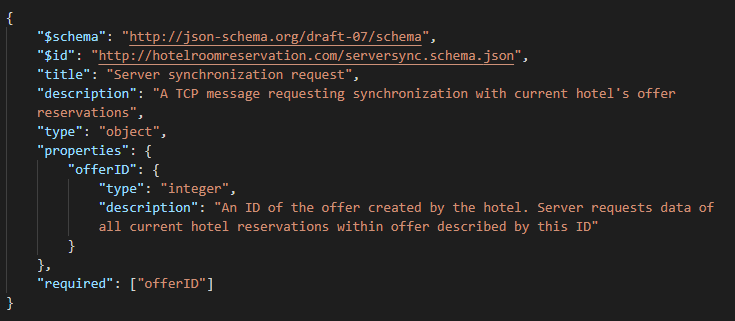
\includegraphics[width=\linewidth]{Hotel login + synchronizacja/server_sync_request.png}
\indent Wiadomość ta wiąże się z żądaniem serwera o synchronizację danych z hotelem. Może ono wystąpić w mechanizmie periodycznej synchronizacji danych w celu zachowania spójności danych w obu modułach, w przypadku anulowania rezerwacji lub podczas procesu tworzenia nowej rezerwacji klienckiej po otrzymaniu komunikatu \texttt{OFFER\_UNAVAILABLE} oznaczającego niedostępność oferty. Wiadomość ta ma na celu potwierdzenia lub aktualizację dostępności danej oferty z hotelem. 

Do kodów “akceptowalnych” należą:
\begin{itemize}
    \item \texttt{SERVER\_SYNC\_RESPONSE\_SUCCESS} - wiadomość zwrotna zawierające dane potrzebne do synchronizacji dostępności oferty po stronie serwera. Zawartość wiadomości jest identyczna jak zawartość wiadomości o kodzie operacyjnym \texttt{HOTEL\_SYNC\_REQUEST}
\end{itemize}

\subsection{Zarządzanie ofertami}
\subsubsection{\texttt{OFFER\_ADD\_REQUEST}}

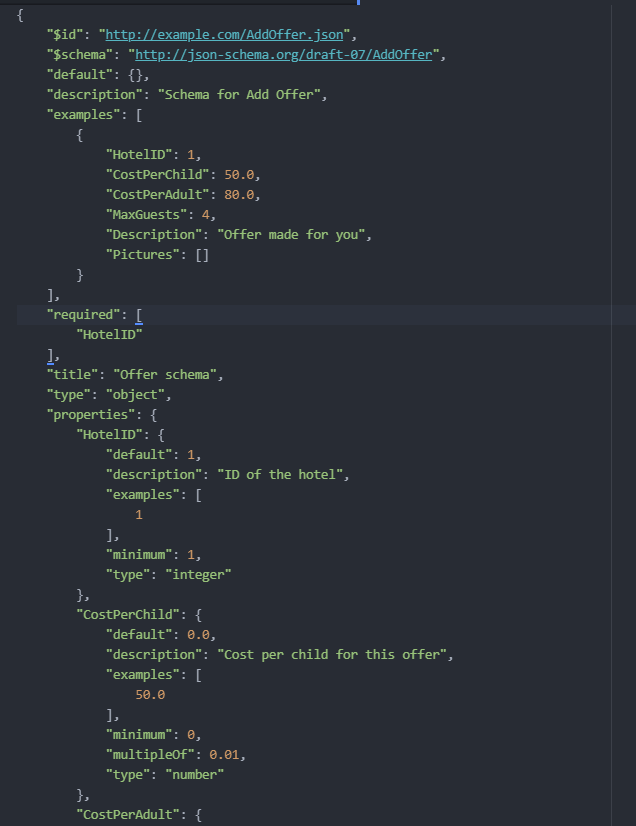
\includegraphics[width=\linewidth]{Oferta-Hotel-Serwer/Offer_Add_JSON1.png}

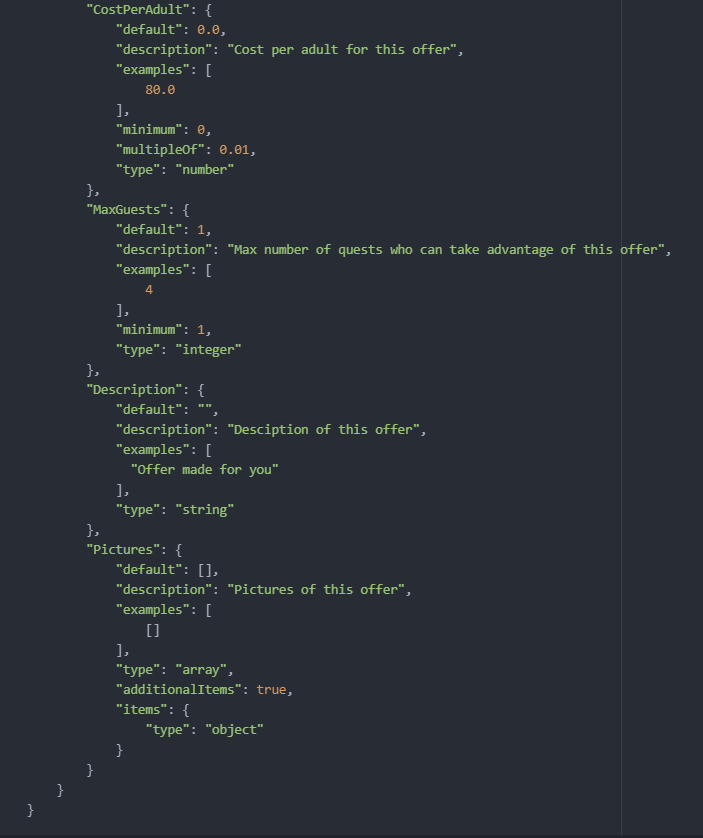
\includegraphics[width=\linewidth]{Oferta-Hotel-Serwer/Offer_Add_JSON2.png}
\textbf{Dodawanie nowej oferty}\\
Proces dodawania nowej oferty zaczyna się od wypełnienia odpowiedniego formularza. Następnie dokonywana jest wstępna walidacja formularza po stronie systemu hotelowego. Jeżeli nie wykryto żadnych błędów, do serwera zostaje przesłany kod operacyjny: \texttt{OFFER\_ADD\_REQUEST} wraz z zserializowanym JSONem zawierającym kolejne pola formularza i informację o ID hotelu od którego pochodzi żądanie. Są to więc kolejno:
\begin{itemize}
    \item CostPerChild - koszt skorzystania z oferty dla dziecka. Powinien być większy od 0. Przyjęta precyzja to 0.01. Parametr ten nie jest wymagany.
    \item CostPerAdult - koszt skorzystania z oferty dla osoby dorosłej. Powinien być większy od 0. Przyjęta precyzja to 0.01. Parametr ten nie jest wymagany.
    \item MaxGuests - maksymalna liczba osób dla której przeznaczona jest oferta. Minimalna wartość to 1. Parametr ten nie jest wymagany.
    \item Description - szczegółowy opis oferty. Parametr ten nie jest wymagany.
    \item Pictures - zdjęcia związane z dodawaną ofertą. Parametr ten nie jest wymagany.
\end{itemize}
Wszystkie parametry dla których wartość nie została zdefiniowana są ukrywane w widoku oferty. Manager hotelu ma możliwość późniejszej edycji oferty i wprowadzenie dokładnych wartości.

\subsubsection{\texttt{OFFER\_ADD\_SUCCESS}}
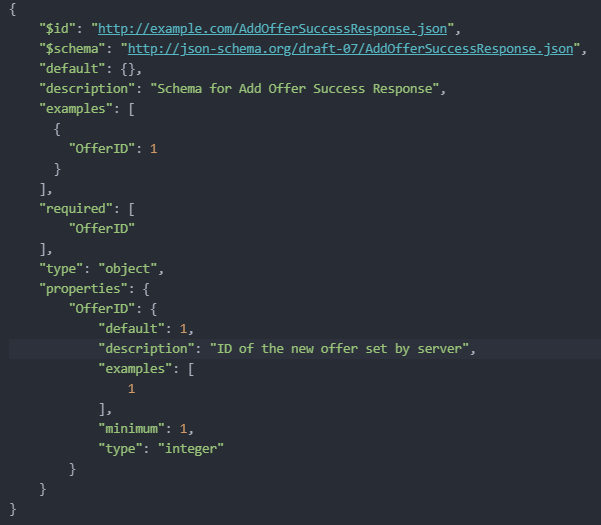
\includegraphics[width=\linewidth]{Oferta-Hotel-Serwer/Offer_Add_Success.png}
Po otrzymaniu JSONa z informacjami o ofercie serwer dokonuje ponownej walidacji wszystkich parametrów. Jeśli oferta została uzupełniona poprawnie serwer dodaje ją do swojej lokalnej bazy danych i odsyła do hotelu informację o powodzeniu w postaci kodu operacyjnego: \texttt{OFFER\_ADD\_SUCCESS} i informacji o ID nowo dodanej oferty. Moduł hotelowy następnie dodaję do lokalnej bazy danych ofertę ze wskazanym przez serwer OfferID. Takie rozwiązani pozwala na zachowanie spójności pomiędzy numerami identyfikacyjnymi ofert po stronie serwera i hotelu.
\subsubsection{\texttt{OFFER\_ADD\_FAILURE}}
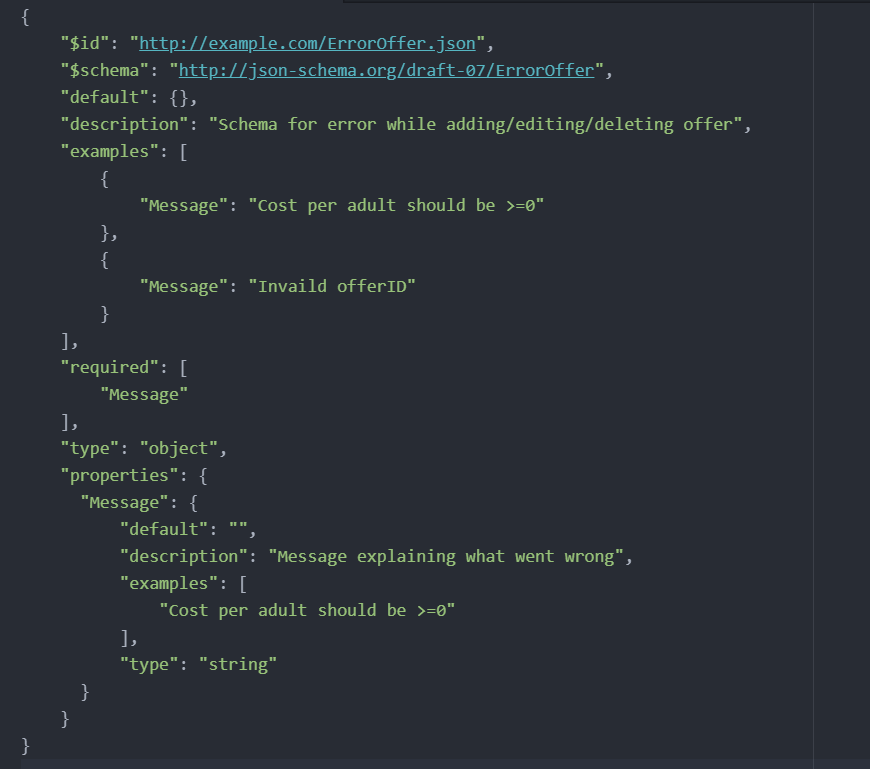
\includegraphics[width=\linewidth]{Oferta-Hotel-Serwer/Offer_Error.png}
W przypadku błędów w formularzu serwer przesyła kod operacyjny: \texttt{OFFER\_ADD\_FAILURE} wraz z JSONem zawierającym jedynie informację na czym polegał błąd. Otrzymany JSON powinien być więc zgodny z powyższym schematem.
Przykładowe błędy to między innymi:
\begin{itemize}
    \item Brak HotelID lub jego nieprawidłowa wartość
    \item Błędne wypełnienie jednego lub więcej pól formularza - niespełnienie warunków walidacji 
\end{itemize}

\subsubsection{\texttt{OFFER\_DELETE\_REQUEST}}
\textbf{Usuwanie oferty}\\
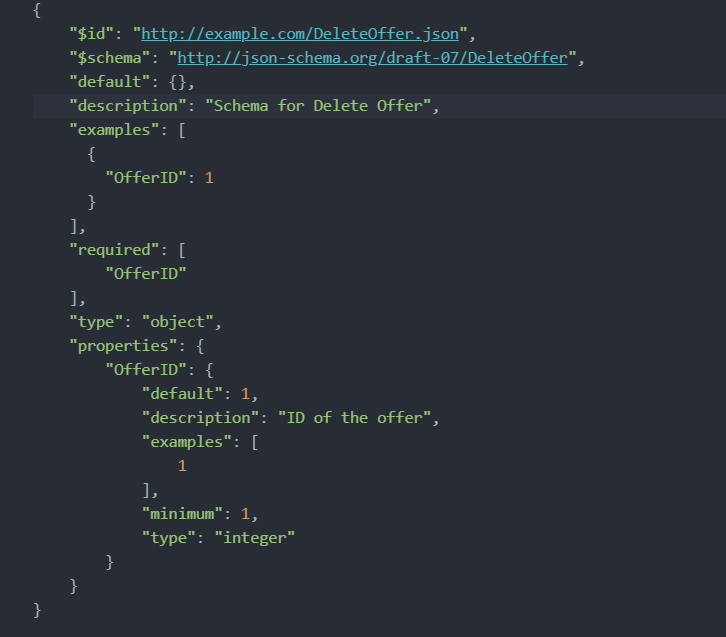
\includegraphics[width=\linewidth]{Oferta-Hotel-Serwer/Offer_DeleteJSON.png}
Manager hotelu wskazuje ofertę przeznaczoną do usunięcia. System hotelowy następnie przesyła kod operacyjny \texttt{OFFER\_DELETE\_REQUEST} wraz z zserializowanym JSONem zawierającym ID usuwanej oferty.

\subsubsection{\texttt{OFFER\_DELETE\_SUCCESS}}
Po otrzymaniu JSONa serwer podejmuje próbę usunięcia ze swojej lokalnej bazy danych oferty o wskazanym ID. Jeśli operacja ta powiodła się, do systemu hotelowego odsyłana jest informacja o powodzeniu w postaci kodu operacyjnego: \texttt{OFFER\_DELETE\_SUCCESS}. 
\subsubsection{\texttt{OFFER\_DELETE\_FAILURE}}
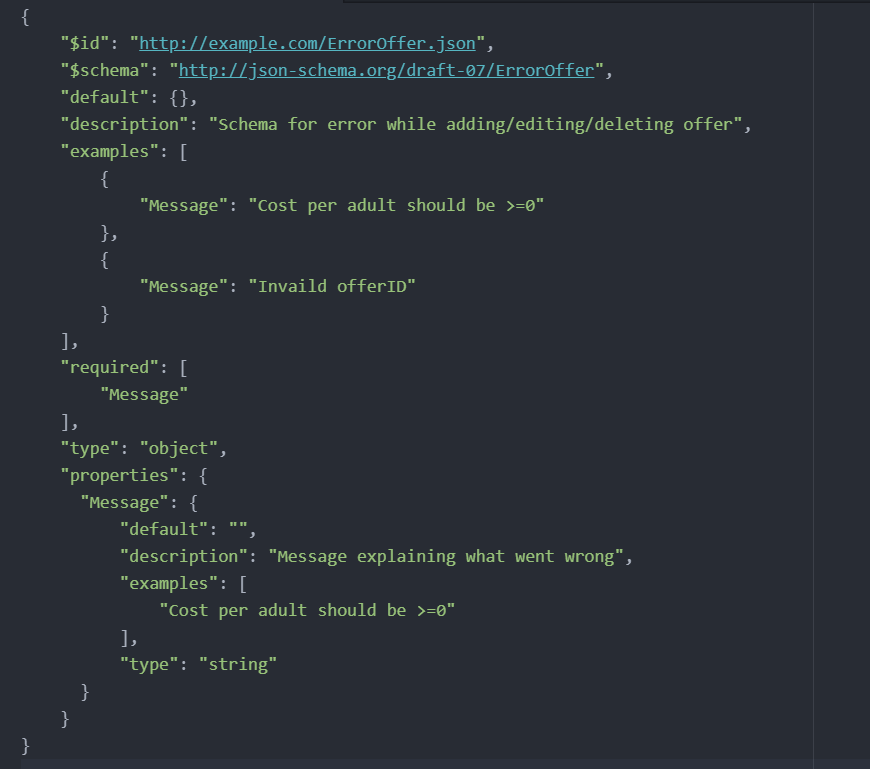
\includegraphics[width=\linewidth]{Oferta-Hotel-Serwer/Offer_Error.png}
Jeśli otrzymany JSON zawiera nieprawidłowe ID, serwer przekona się o tym przy próbie znalezienia zadanego rekordu o zadanym ID. System hotelowy zostanie poinformowany o zaistniałym błędzie poprzez przesłanie następującego kodu operacyjnego: \texttt{OFFER\_DELETE\_FAILURE} wraz ze stosownym komunikatem.
W przypadku wystąpienia błędów po stronie serwera, system hotelowy zostanie poinformowany o zaistniałej sytuacji analogicznie kodem \texttt{OFFER\_DELETE\_FAILURE} wraz z JSONem zawierającym jedynie informację na czym polegał błąd. Niezależnie od natury błędu otrzymany JSON powinien być więc zgodny z powyższym schematem.
\newpage
\subsubsection{\texttt{OFFER\_EDIT\_REQUEST}}
\textbf{Edytowanie istniejącej oferty}\\
\begin{center}
    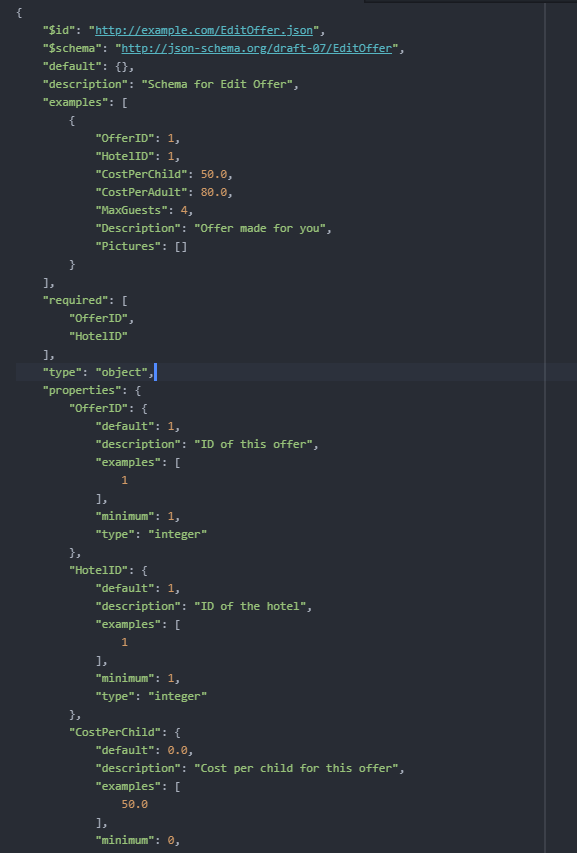
\includegraphics[scale=1.3]{Oferta-Hotel-Serwer/Offer_Edit_JSON1.png}
    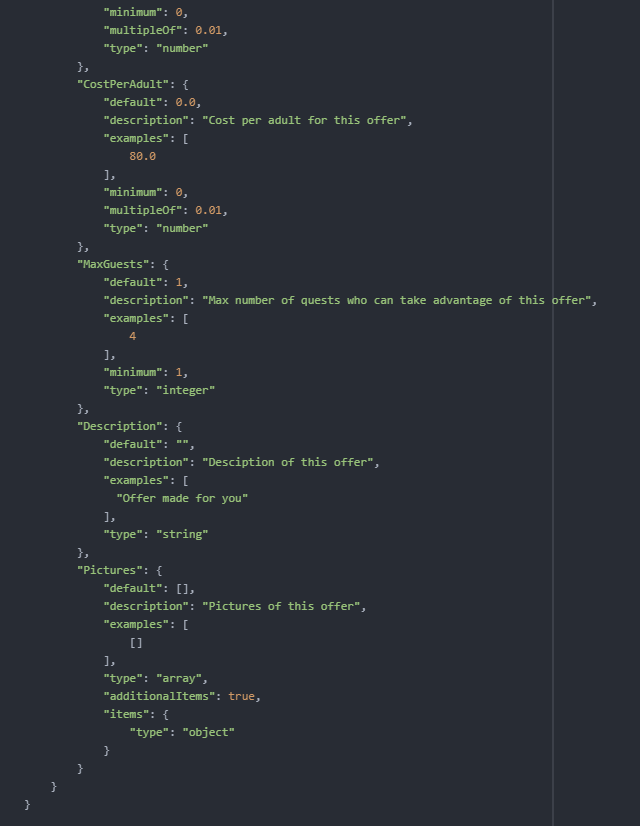
\includegraphics[width=\linewidth]{Oferta-Hotel-Serwer/Offer_Edit_JSON2.png}
\end{center}

Manager ma możliwość edycji już istniejącej oferty. W tym celu wybiera ofertę i przechodzi do jej edycji poprzez formularz znany mu dobrze z dodawania nowej oferty. Po zakończeniu edycji oferta jest ponownie walidowana po stronie systemu hotelowego, po czym do serwera zostaje przesłany kod operacyjny: \texttt{EDIT\_OFFER\_REQUEST} wraz z zserialiozowanym JSONem zawierającym pola które zostały poddane modyfikacji. Schemat wiadomości jest więc analogiczny do tego dla dodawania nowej oferty. Wzbogacony jest jedynie o dodatkowe wymagane pole OfferID pozwalające na identyfikację modyfikowanej oferty.
\subsubsection{\texttt{OFFER\_EDIT\_SUCCESS}}
Po otrzymaniu JSONa z informacjami o ofercie serwer dokonuje ponownej walidacji wszystkich parametrów. Jeśli oferta została zedytowana poprawnie serwer uaktualnia odpowiedni wpis w swojej lokalnej bazie danych i odsyła do systemu hotelowego informację o powodzeniu w postaci kodu operacyjnego: \texttt{OFFER\_EDIT\_SUCCESS}. 
\subsubsection{\texttt{OFFER\_EDIT\_FAILURE}}
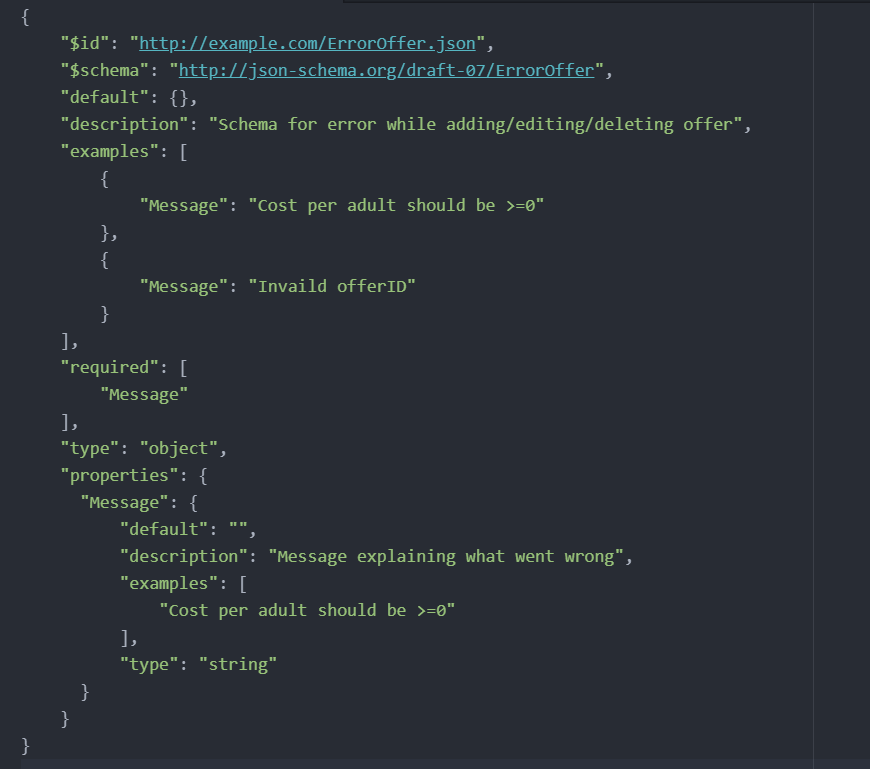
\includegraphics[width=\linewidth]{Oferta-Hotel-Serwer/Offer_Error.png}
W przypadku błędów w formularzu serwer przesyła kod operacyjny: \texttt{OFFER\_EDIT\_FAILURE} wraz z JSONem zawierającym jedynie informację na czym polegał błąd.

\subsection{Zarządzanie rezerwacjami}

\subsubsection{\texttt{RESERVATION\_CREATE}} \label{reservation_info}
Komunikat przesyła szczegółowe informacje dot. rezerwacji. Serwer wysyła tę wiadomość natychmiast po prośbie klienta stworzenia tejże rezerwacji.

Pola tego obiektu są analogiczne do odpowiadającej mu klasy \texttt{ReservationInfo}, rozszerzone o \texttt{ClientID} klienta powiązanego z rezerwacją.

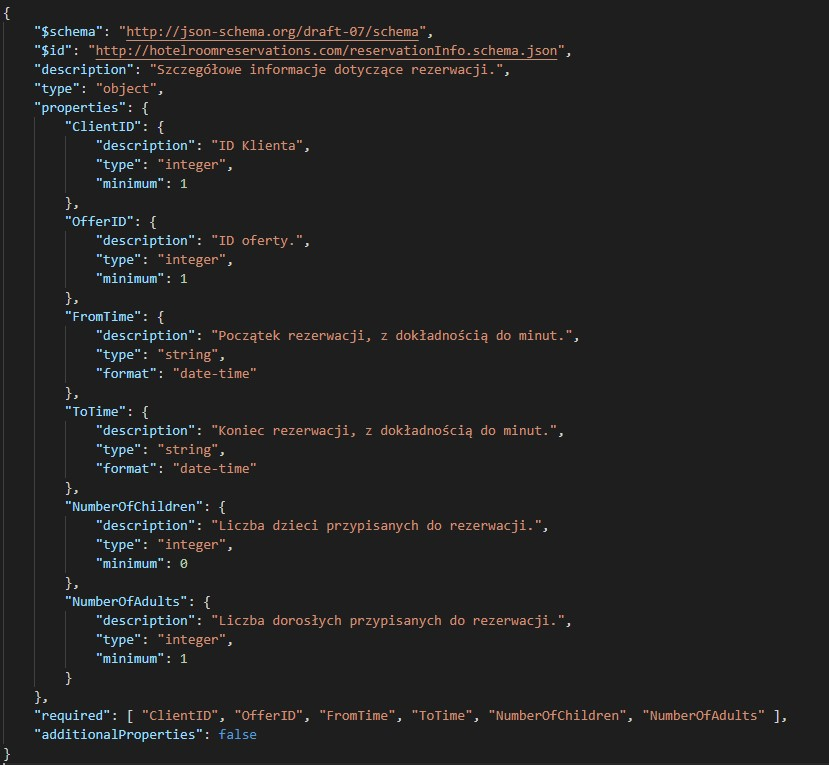
\includegraphics[width=\linewidth]{Rezerwacje/ReservationInfoSchema.jpg}

Oczekiwane odpowiedzi:
\begin{itemize}
    \item \texttt{OFFER\_UNAVAILABLE} \\
    Oferta jest niedostępna w wybranym okresie wg danych po stronie hotelu. Hotel sugeruje, że potrzebna jest synchronizacja.
    \item \texttt{PAYMENT\_INFO} \\
    Serwer po otrzymaniu \texttt{PAYMENT\_INFO} zapisuje otrzymane informacje tymczasowo w lokalnej bazie danych. Oprócz otrzymanych danych serwer przetrzymuje w danym wierszu również informację o ID hotelu, od którego je otrzymał. W ten sposób może jednoznacznie zidentyfikować rezerwację, w ramach której została utworzona dana płatność (innymi słowy, para [HotelID,~ReservationID] jest tutaj kluczem głównym). Informacje te są potrzebne głównie dla późniejszego wykorzystania przez klienta przy płatności (patrz: /payments).
    
    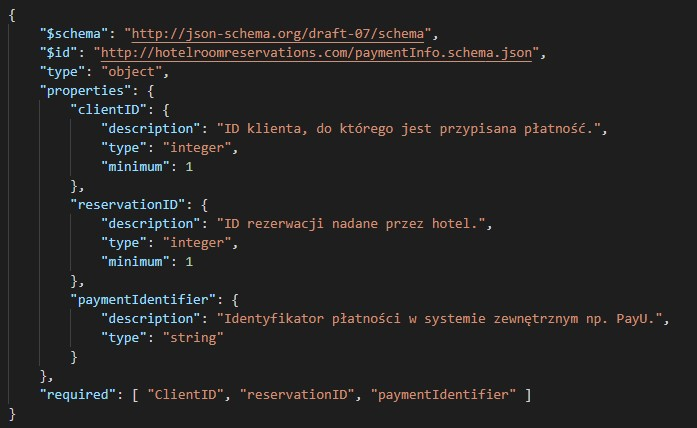
\includegraphics[width=\linewidth]{Rezerwacje/paymentInfo.jpg}
\end{itemize}

\subsubsection{\texttt{PAYMENT\_SUCCESS}} \label{payment_success}
Komunikat wysyłany do hotelu po otrzymaniu od klienta informacji o zakończonym procesie płatności.

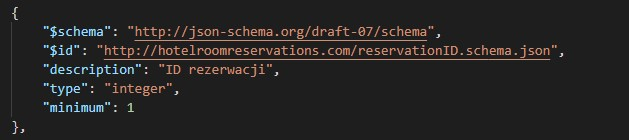
\includegraphics[width=\linewidth]{Rezerwacje/reservationIDSchema.jpg}

Oczekiwane odpowiedzi:
\begin{itemize}
    \item \texttt{PAYMENT\_SUCCESS\_RESPONSE\_SUCCES}\\
    Płatność dotarła do hotelu. Hotel w odpowiedzi przesyła obiekt z 2 właściwościami: \textbf{ID rezerwacji} oraz \textbf{ID klienta}. Serwer zapisuje te informacje w swojej bazie.
    \item \texttt{PAYMENT\_SUCCESS\_RESPONSE\_FAILURE}\\
    Płatność nie dotarła do hotelu. Wiadomość zawiera string w opisanym powodem błędu.
    \item \texttt{ID\_UNKNOWN}\\
    Nieznane ID rezerwacji
\end{itemize}

\subsubsection{\texttt{RESERVATION\_DELETE}}
    Klient może zrezygnować ze swojej rezerwacji w dowolnym momencie. Zaraz po otrzymaniu przez serwer takiej prośby, przekazuje ją do hotelu niniejszym komunikatem. Wewnątrz wiadomości znajduje się ID rezerwacji, której dotyczy. Struktura jest więc identyczna jak w (\ref{payment_success}).
    
Oczekiwane odpowiedzi:
\begin{itemize}
    \item \texttt{RESERVATION\_DELETE\_SUCCESS}\\
    Usunięcie powiodło się.
    \item \texttt{RESERVATION\_DELETE\_FAILURE}\\
    Usunięcie nie powiodło się.
    \item \texttt{ID\_UNKNOWN}\\
    Nieznane ID rezerwacji.
\end{itemize}

\subsubsection{\texttt{RESERVATION\_GET}}
Zapytanie o szczegóły konkretnej rezerwacji - na przykład w celu przekazania tych informacji klientowi. Struktura wiadomości identyczna jak w (\ref{payment_success}).

Oczekiwane odpowiedzi:
\begin{itemize}
    \item \texttt{RESERVATION\_GET\_RESPONSE}\\
    Szczegółowe info. dot. rezerwacji. Struktura wiadomości identyczna jak w komunikacie \texttt{RESERVATION\_CREATE }(patrz: \ref{reservation_info}).
    \item \texttt{ID\_UNKNOWN}\\
    Nieznane ID rezerwacji.
\end{itemize}

\section{Klient-Serwer}
\indent \indent Komunikacja pomiędzy klientem (modułem aplikacji klienckiej), a serwerem odbywa się przy użyciu połączeń HTTP i REST API. Poniżej opisane są wszystkie endpoint'y oraz związane z nimi żądania i odpowiedzi HTTP zamodelowane w RAML.
\subsection{Autentykacja i autoryzacja}
\indent \indent Poniżej opisana jest przykładowa implementacja schematu autentykacji dla klientów realizowana przez serwer. Część ta jest jedynie przykładem realizacjitego procesu - inną możliwością jest użycie zewnętrznych usług autentykacyjnych. Wówczas cały proces autentykacji byłby realizowany oddzielnie, natomiast serwer przechowywałby jedynie dane klientów bez ich sekretów. Wówczas na podstawie zewnętrznego dostawcy token'ów JWT (np. Azure B2C) na podstawie claim'ów zawartych w tym tokenie możliwe byłoby przydzielenie własnego niestandardowego token'a (opisanego poniżej) identyfikującego klienta z rekordem w bazie danych klienta.\\
\indent Wszystkie endpointy serwera (poza endpointem związanym z logowaniem) zabezpieczone są przez schemat autentykacji opierający się na tworzeniu tokenów autentykacyjnych dla każdego klienta w momencie gdy dostarczone zostaną poprawne dane logowania. W każdym zapytaniu klienta powinien być dołączony nagłówek “x-session-token”, którego wartością jest otrzymany przez klienta token autentykacyjny. Token ten jest zawsze tworzony po stronie serwera i odpowiednio szyfrowany w celu uniemożliwienia jego modyfikacji bądź podrobienia. Generowany token ma format JSON i jego przykładowa zawartość jest podana na zdjęciu poniżej. Token “clientSessionToken” jest obiektem JSON zawierającym właściwość, której wartością jest ciąg znaków będący zaszyfrowanym tokenem JWT, natomiast “serverSessionToken” powstaje poprzez rozszyfrowanie przez serwer tego ciągu znaków. Każdy token zawiera właściwość “id”, której wartość jednoznacznie identyfikuje klienta w bazie danych serwera.
\newline
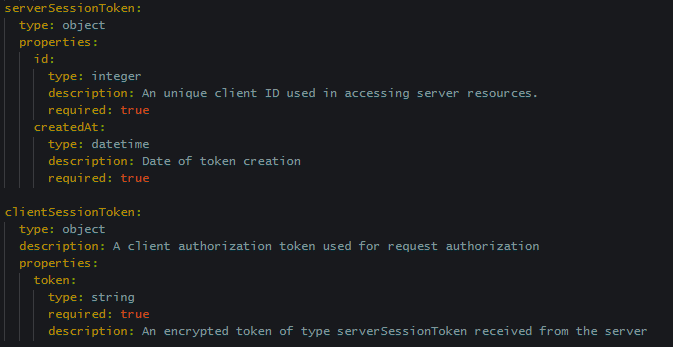
\includegraphics[width=\linewidth]{Client login + authentication/authentication_tokens.png}
\indent Poniżej znajduje się dokładny opis schematu autentykacji w języku RAML oraz zwracane kody błędu związane z niepowodzeniem procesu uwierzytelnienia klienta. Każda wiadomość związana z błędem zawiera dokładny opis zawierający czytelne dla człowieka szczegóły dotyczące tego błędu.
\newline
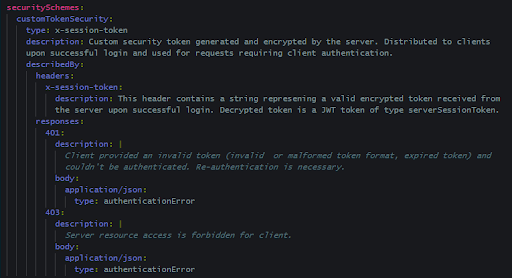
\includegraphics[width=\linewidth]{Client login + authentication/authentication_scheme.png}
\newline
\newline
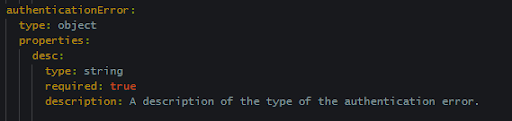
\includegraphics[width=\linewidth]{Client login + authentication/authentication_error.png}

\subsection{Logowanie klienta i pobieranie danych o kliencie}
\indent \indent Z logowaniem klienta jest związana rejestracja konta. Proces rejestracji nie jest przedstawiony w specyfikacji, gdyż może być on zrealizowany w dowolny sposób. Przykładową implementacją może być tabela sekretów klienta w module serwerowym na podstawie której serwer przeprowadza proces autentykacji, bądź proces rejestracji może być częścią usług zewnętrznej, w skład której wchodzi proces autentykacji i zarządzanie sekretami klientów (np. serwis Azure B2C). Poniżej przedstawiona została przykładowa implementacja logowania klientów w przypadku implementacji procesu autentykacji przeprowadzanej przez serwer w oparciu o lokalną tablicę sekretów w bazie danych. Porównywane są wówczas przesłane przez klienta login i hasło z danymi przechowywanymi w takiej tabeli i zwracany jest odpowiednio zaszyfrowany token przechowujący ID klienta.\\
\indent Do zarządzania danymi związanymi z kontem klienta oraz logowania do serwisu służą odpowiednio endpointy: \texttt{/Client} oraz \texttt{/Client/login}. Endpoint \texttt{/Client} jest zabezpieczony wyżej zdefiniowanym schematem autentykacji, natomiast endpoint służący do logowania nie wymaga przesyłania nagłówka \texttt{x-session-token}.

\subsubsection{\texttt{/Client}}

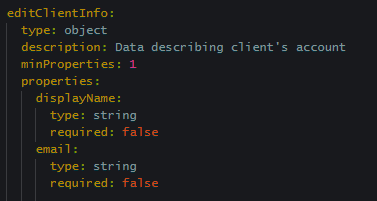
\includegraphics[width=\linewidth]{Client login + authentication/client_info_type.png}
\newpage
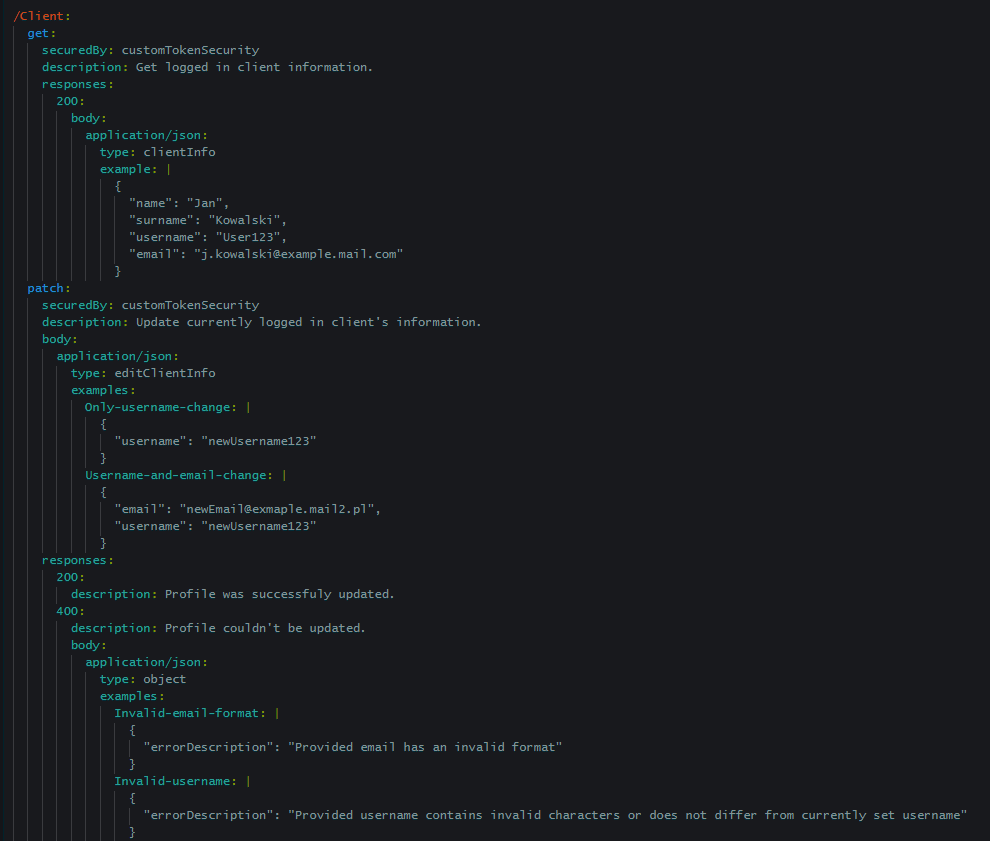
\includegraphics[width=\linewidth]{Client login + authentication/client_info.png}
\indent Endpoint ten definiuje 2 metody HTTP: \texttt{GET} oraz \texttt{PATCH}. Metoda \texttt{GET} pobiera informacje o aktualnie zalogowanym użytkowniku, natomiast metoda \texttt{PATCH} udostępnia możliwość zmiany danych użytkownika takich jak e-mail lub nazwa użytkownika. W przypadku niepowodzenia metody \texttt{PATCH} wysyłany jest obiekt JSON z właściwością "errorDescription" opisującą rodzaj błędu.

\subsubsection{\texttt{/Client/login}}
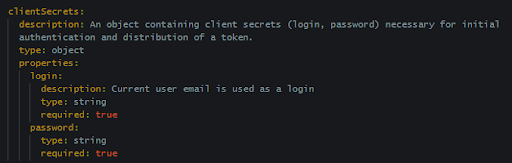
\includegraphics[width=\linewidth]{Client login + authentication/client_secrets.png}
\newline
\includegraphics[width=\linewidth]{Client login + authentication/client_login.png}
\indent Endpoint ten nie jest zabezpieczony przez schemat autentykacji - nie jest wymagane dołączanie tokenu do nagłówka “x-session-token”.
\newline
\indent Endpoint służący do logowania się użytkowników do systemu za pomocą ustalonego przy rejestracji loginu i hasła. Wysłane przez klienta dane logowania jako metoda POST sprawdzane są następnie przez serwer. W przypadku sukcesu tworzony jest “serverSessionToken” zawierający “id” logującego się klienta i szyfrowany a następnie zwracany w ciele odpowiedzi HTTP serwera. W celu dalszej autentykacji klienta token ten jest dołączany do kolejnych żądań HTTP w nagłówku “x-session-token”. W przypadku niepowodzenia serwer zwraca odpowiedni kod błędu oraz dokładny opis błędu w ciele odpowiedzi HTTP.
Powyżej znajdują się szczegółowe opisy typów danych oraz żądań i odpowiedzi HTTP w języku RAML.

\subsection{Wyszukiwanie hoteli}

    \includegraphics[width=\linewidth]{Oferta+Hotel-Raml/pageable.png}

 Opisane w tej i kolejnej sekcji endpointy \texttt{/Hotel} i \texttt{/Hotel/\{HotelID\}/Offer} korzystają z pagingu. Rozwiązanie to zwiększa czytelność zwracanych list ograniczając liczbę wyników do ilości zdefiniowanej przez parametr: limit. Przeglądanie kolejnych stron odbywa się przez modyfikacje parametru: offset.
\subsubsection{\texttt{/Hotel}}
\begin{center}
    \includegraphics[scale=1.3]{Oferta+Hotel-Raml/Hotel_Raml.png}
\end{center}

\newpage
\includegraphics[width=\linewidth]{Oferta+Hotel-Raml/HotelInfoPreview_Raml.png}
Endpoint służy do przeglądania hoteli współpracujących z systemem. Dostęp jest stosownie chroniony przez customSecurityToken. W celu zwiększenia przejrzystości zastosowano paging ograniczający ilość rekordów znajdujących się na aktualnie przeglądanej stronie. Ponadto użytkownik ma możliwość wyszukiwania wymarzonego hotelu po zestawie filtrów takich jak lokalizacja, czy nazwa hotelu. Wynikiem udanego wyszukiwania hoteli jest kod 200 wraz z listą zawierającą obiekty typu HotelInfoPreview. Każdy z elementów listy składa się wyłącznie z kluczowych informacji na temat hotelu co poprawia czytelność wyników wyszukiwania. Są to odpowiednio opis hotelu i jego lokalizacja. Naciśnięcie na jeden z elementów listy powoduje przeniesienie do enpoint'u \texttt{/Hotel/\{HotelID\}} gdzie uzyskujemy dostęp do dalszych interakcji z wybranym przez nas hotelem.\\
W przypadku niepowodzenia zwracany jest błąd o kodzie 400 wraz ze stosownym opisem.
\subsubsection{\texttt{/Hotel/\{HotelID\}}}
\includegraphics[width=\linewidth]{Oferta+Hotel-Raml/HotelID_Raml.png}
\newpage
\includegraphics[width=\linewidth]{Oferta+Hotel-Raml/HotelInfo_Raml.png}
Po wybraniu z listy konkretnego hotelu mamy dostęp do większej ilości informacji w ramach przygotowanego przez hotel opisu. O powodzeniu jesteśmy również informowani przez kod 200. Uzyskujemy także dostęp do dalszych działań związanych z wybranym przez nas hotelem. W przypadku wybrania ID nieistniejącego hotelu użytkownik jest informowany o błędzie przez kod 404 i stosowny komentarz.

\subsection{Wyszukiwanie ofert}
\subsubsection{\texttt{/Hotel/\{HotelID\}/Offer}}
\includegraphics[width=\linewidth]{Oferta+Hotel-Raml/Offer_e_Raml.png}
\newpage
\includegraphics[width=\linewidth]{Oferta+Hotel-Raml/OfferPreview_Raml.png}
Zadaniem tego endpointu jest prezentacja ofert należących do wybranego przez użytkownika we wcześniejszych krokach hotelu. Analogicznie jak w przypadku opisanego wyżej endpointu \texttt{/Hotel} w celu podniesienia przejrzystości zastosowano paging i wyświetlane są jedynie najistotniejsze informacje dotyczące prezentowanych ofert. Między innymi: koszt skorzystania z oferty dla dziecka i osoby dorosłej, a także maksymalna liczba gości, która może skorzystać z oferty. Użytkownik aplikacji przy wyszukiwaniu wymarzonej oferty ponownie może skorzystać z zestawu filtrów. Poprawne wyszukiwanie ofert kończy się, więc zwróceniem kodu 200 wraz z listą obiektów typu OfferPreview przedstawionych na powyższym schemacie. O niepoprawnym użyciu filtrów czy błędzie innej postaci informuje kod 400 wraz ze stosownym komentarzem.
\subsubsection{\texttt{/Hotel/\{HotelID\}/Offer/\{OfferID\}}}
\includegraphics[width=\linewidth]{Oferta+Hotel-Raml/OfferID_Raml.png}
\newpage
\begin{center}
    \includegraphics[scale=1]{Oferta+Hotel-Raml/Offer_Raml.png}
\end{center}

Po wybraniu z listy konkretnej oferty możemy poznać jej szczegóły takie jak opis, zdjęcia czy opinie innych użytkowników aplikacji, którzy skorzystali już z tej oferty. Przykładowy obiekt Offer zwracany w przypadku poprawnego OfferID został przedstawiony na powyższej grafice ilustrującej cały endpoint. W przypadku wskazania oferty o nieprawidłowym OfferID jesteśmy informowani o błędzie przez kod 404 wraz ze stosownym komentarzem.

\subsection{Zarządzanie rezerwacjami}
Ze szczególną uwagą warto przyjrzeć się komunikatom wymienianym pod adresem \texttt{/Reservations/} oraz \texttt{/Payments/}. 
Ze względu na to, że potencjalna strona z listą rezerwacji użytkownika stanowi jego "centrum dowodzenia wszechświatem" i za jej pośrednictwem user wykonuje wiele akcji, warto dobrze zrozumieć wymianę komunikatów odbywającą się w tym miejscu. Pewne nieoczywiste rozwiązania zastosowane są m.in. przy płatnościach.

\subsubsection{\texttt{/Reservations}}
Pod tym adresem można otrzymać wszystkie rezerwacje klienta wraz z ewentualnymi przypisanymi do nich opiniami. \texttt{HotelID} i \texttt{ReservationID} reprezentują wspólnie jedną rezerwację. Są niejako złożonym kluczem głównym dla rezerwacji. Jeżeli dana rezerwacja nie posiada wystawionej opinii, właściwość \texttt{ReviewID} nie jest zawarta w przesłanych danych (patrz przykład).

\includegraphics[width=\linewidth]{Rezerwacje/reservationType.jpg}

\includegraphics[width=\linewidth]{Rezerwacje/reservationsGET.jpg}
Należy zauważyć, że nie jest to pełna lista informacji gotowa do wyświetlenia, a raczej lista powiązanych ze sobą ID. Aby otrzymać taką listę, należy odwołać się do adresu \texttt{/Reservations/\{HotelID\}/\{ReservationID\}} reprezentującego konkretną rezerwację - należy to wykonać dla \textit{każdej} otrzymanej rezerwacji.

Przesłanie prośby o dodanie nowej rezerwacji odbywa się przez metodę \texttt{POST}. Wysyła się obiekt \texttt{ReservationInfo} zawierający wszystkie niezbędne informacje.

\includegraphics[width=\linewidth]{Rezerwacje/reservationInfoType.jpg}

\includegraphics[scale=0.6]{Rezerwacje/reservationsPOST.jpg}

\subsubsection{\texttt{/Reservations/\{HotelID\}/\{ReservationID\}}}
Pod tym endpointem można znaleźć szczegółowe informacje dotyczące konkretnej rezerwacji \texttt{ReservationID} w hotelu \texttt{HotelID} bądź ją usunąć.

\includegraphics[width=\linewidth]{Rezerwacje/reservationEndpoint.jpg}

\subsubsection{\texttt{/Payments}} \label{payments}
Powyżej nie znajdują się jednak \textit{wszystkie} informacje dotyczące rekordu. Identyfikatory płatności przypisane do rejestracji są przechowywane pod osobnym adresem URI. Serwer przechowuje te informacje jedynie przez krótką chwilę, natomiast dłużej są przetrzymywane w Hotelu (przynajmniej do zakończenia rezerwacji). W momencie, kiedy serwer otrzymuje komunikat \texttt{PAYMENT\_INFO} (patrz (\ref{reservation_info}) oraz spójrz na (\ref{reservation_diagram})), zapisuje te informacje u siebie. Aby klient mógł opłacić zamówienie, musi dostać te informacje - w związku z tym przy listowaniu rezerwacji należy również się odwołać do \texttt{/Payments}. Kiedy klient szczęśliwie zakończy opłatę, informuje o tym serwer, który informuje hotel, po czym serwer usuwa informację o tej płatności. Hotel może przechowywać identyfikator płatności (i tak też robi, w razie ewentualnych zwrotów) przez dłuższy czas.\\
\indent Trudna sytuacja może pojawić się w przypadku, kiedy płatność nie zostanie potwierdzona przez hotel. Wówczas stan rzeczy jest następujący:
\begin{itemize}
    \item Hotel stworzył płatność i oznaczył ją jako nieudaną (znacznik bool isError). Przechowuje u siebie dane zarówno o płatności jak i rezerwacji.
    \item Płatność nie została zakończona, więc serwer nie zapisał sobie tej rezerwacji. Posiada natomiast wpis dot. płatności (z flagą isError), który pozostawił (ponieważ dostał odpowiedź\\ \texttt{PAYMENT\_SUCCESS\_RESPONSE\_FAILURE}).
    \item Aplikacja kliencka wyświetliła komunikat z sugestią kontaktu z hotelem. Po przeładowaniu interfejsu komunikatu nie ma.
\end{itemize}
Aby uchronić się przed tym, że użytkownik straci jakiekolwiek informacje o tej rezerwacji (oraz pieniądze) – serwer powinien dla każdej płatności oznaczonej flagą \texttt{isError}, poprosić hotel o te dane wysyłając \texttt{RESERVATION\_GET}.

\includegraphics[width=\linewidth]{Rezerwacje/paymentsGET.jpg}

\includegraphics[scale=0.7]{Rezerwacje/paymentsDELETE.jpg}

\textbf{Uwaga!} Dla uproszczenia projektu, aby nie trzeba było wprowadzać czwartego modułu zajmującego się płatnościami, proces w systemie jest symulowany w bardzo prosty sposób: zawsze się udaje. W aktualnym inkremencie rozwoju nie przewidujemy zwracanego błędu 409 metody \texttt{/Payments DELETE} - poza specjalnie zaaranżowanym przypadkiem testowym.

\subsection{Zarządzanie opiniami}
Endpointy poniżej służą użytkownikowi do zarządzania swoimi opiniami na temat rezerwacji które odbył.
Oba są zabezpieczone w sposób przedstawiony na początku tego rozdziału.\newline
\begin{center}
    \includegraphics[scale=0.7]{Review+id/return_id.png}
    \includegraphics[scale=0.7]{Review+id/review.png}
\end{center}
Powyżej widzimy szczegółowy opis typów używanych przez opisane poniżej Endpointy w języku RAML. typ review służy do przesyłani informacji o Opinii i jest odpowiednikiem klasy Review w systemie. Natomiast id\_return służy do przesyłania id świeżo dodanej opinii do klienta.
\subsubsection{\texttt{/Review}}

\includegraphics[width=\linewidth]{Review+id/post.png}
\newline
\includegraphics[width=\linewidth]{Review+id/get[].png}

Endpoint służy do pobierania wszystkich Opinii klienta oraz dodawaniu nowych.
Metoda POST nie znajduje się w \texttt{/Review/\{id\}}, gdyż nie znamy jeszcze id Opinii. Zostanie ona przyznana przez serwer i odesłana do klienta za pomocą id\_return. Aplikacja kliencka zapisuje po uzyskaniu id zapisuje nową Opinię razem z innymi.
Metoda GET jest tutaj używana zaraz po logowani Klienta w celu pobrania jego opinii.
\subsubsection{\texttt{/Review/\{id\}}}
\begin{center}
    \includegraphics[width=\linewidth]{Review+id/get.png} \newline
    \includegraphics[width=\linewidth]{Review+id/put.png} \newline
    \includegraphics[width=\linewidth]{Review+id/delete.png}\newline
\end{center}
Endpoint służy do zarządzania pojedynczą Opinią.

Metoda GET służy pobieraniu pojedynczej Opinii z Serwera.

Metod PUT służy do edytowani istniejących w systemie Opinii. Zastępuje ona dane w Serwerze danymi przesłanymi z Aplikacji Klienckiej.

Metoda DELETE natomiast usuwa z systemu Opinię o danym id.

\section{Scenariusze testowe}
Scenariusze przedstawiają proponowane testy do przeprowadzania na systemie. Podają one na początku dane wejściowe, następnie przebieg wykonywania zadania oraz ewentualne scenariusze alternatywne (w razie błędów). Scenariusze są przygotowane w ten sposób aby można było łatwo przetestować poprawność zaimplementowanego systemu pod kątem komunikacji - poniższe scenariusze pokrywają jej całość.

\subsection{Dodawanie nowej oferty}
Manager hotelu dodaje nową ofertę. Moduły pomiędzy którymi odbywa się komunikacja: Hotel, Serwer. Hotel w ramach którego manager dokonuje operacji ma następujące ID:
\begin{itemize}
    \item HotelID: 1
\end{itemize}
Formularz został wypełniony następującymi danymi: 
\begin{itemize}
    \item Cost per child: 80
    \item Cost per adult: 120
    \item Max guests: 3
    \item Description: Very very very good offer 
\end{itemize}
Następuje wymiana wiadomości:
\begin{itemize}
    \item Hotel $\rightarrow$ Serwer \texttt{OFFER\_ADD\_REQUEST}\\ 
    Do modułu serwerowego przesłany zostaje zserializowany obiekt oferty. Oferta jest walidowana, a następnie dodawana do lokalnej bazy danych serwera. Powiedzmy, że oferta zostaje dodana do odpowiedniej tabeli z następującym ID:
    \begin{itemize}
        \item OfferID: 3
    \end{itemize}
    \item Hotel $\leftarrow$ Serwer \texttt{OFFER\_ADD\_SUCCESS}\\
    W odpowiedzi odsyłany jest OfferID pod jakim oferta została dodana. Moduł hotelowy następnie dodaje ofertę pod tym samym ID do swojej lokalnej bazy danych.
\end{itemize}
Wynikiem pomyślnego zakończenia operacji jest dodanie do bazy danych serwera i hotelu w stosownych tabelach następującego wpisu:
\begin{itemize}
    \item OfferID: 3
    \item isActive: true
    \item costPerChild: 80
    \item costPerAdult: 120
    \item maxGuests: 3
    \item description: Very very very good offer 
\end{itemize}
Dla serwera wpis ten jest dodatkowo rozszerzony o następujące pole:
\begin{itemize}
    \item HotelID: 1
\end{itemize}
W przypadku gdy:
\begin{itemize}
    \item Dojdzie do utraty połączenia przy przesyłaniu oferty przez moduł hotelowy do serwera. 
    \item Walidacja parametrów oferty po stronie serwera nie zakończy się powodzeniem.
    \item Dojdzie do utraty połączenia przy przesyłaniu odpowiedzi serwera.
    \item Przesyłane wiadomości są niezgodne z przyjętym formatem (kody operacyjne, treść wiadomości).
\end{itemize}
operacja kończy się niepowodzeniem i nowa oferta nie jest dodawana do systemu. Jeśli oferta została już dodana po stronie serwera, z bazy danych usuwany jest dodany rekord. W przypadku błędów przy walidacji do modułu hotelowego odsyłana jest odpowiedź o kodzie \texttt{OFFER\_ADD\_FAILURE} wraz z informacją, które pole zostało błędnie wypełnione.

\subsection{Edycja istniejącej oferty} 
Manager hotelu dokonuje edycji istniejącej już w systemie oferty. Moduły pomiędzy którymi odbywa się komunikacja: Hotel, Serwer. Hotel w ramach którego manager dokonuje operacji ma następujące ID:
\begin{itemize}
    \item HotelID: 1
\end{itemize}
Wybrana przez niego oferta ma następujące ID:
\begin{itemize}
    \item OfferID: 3
\end{itemize}
Formularz został wypełniony następującymi danymi: 
\begin{itemize}
    \item Cost per child: 70
    \item Cost per adult: 110
    \item Max guests: 4
    \item Description: Not so very very very good offer 
\end{itemize}
Następuje wymiana wiadomości:
\begin{itemize}
    \item Hotel $\rightarrow$ Serwer \texttt{OFFER\_EDIT\_REQUEST}\\ 
    Do modułu serwerowego przesłany zostaje zserializowany obiekt oferty. Oferta jest walidowana, a następnie uaktualniany jest stosowny wpis w bazie danych serwera. 
    \item Hotel $\leftarrow$ Serwer \texttt{OFFER\_EDIT\_SUCCESS}\\
    Po otrzymaniu potwierdzenia moduł hotelowy uaktualnia wpis z daną ofertą w swojej lokalnej bazie danych
\end{itemize}
Wynikiem pomyślnego zakończenia operacji jest uaktualnienie wpisu zawierającego informacje o wskazanej ofercie dla baz danych serwera i hotelu:
\begin{itemize}
    \item OfferID: 3
    \item isActive: true
    \item costPerChild: 70
    \item costPerAdult: 110
    \item maxGuests: 4
    \item description: Not so very very very good offer 
\end{itemize}
Dla serwera wpis ten jest dodatkowo rozszerzony o następujące pole:
\begin{itemize}
    \item HotelID: 1
\end{itemize}
W przypadku gdy:
\begin{itemize}
    \item Dojdzie do utraty połączenia przy przesyłaniu oferty przez moduł hotelowy do serwera. 
    \item Walidacja parametrów oferty po stronie serwera nie zakończy się powodzeniem.
    \item Dojdzie do utraty połączenia przy przesyłaniu odpowiedzi serwera.
    \item Przesyłane wiadomości są niezgodne z przyjętym formatem (kody operacyjne, treść wiadomości).
\end{itemize}
operacja kończy się niepowodzeniem i oferta nie ulega modyfikacji. W przypadku błędów przy walidacji do modułu hotelowego odsyłana jest odpowiedź o kodzie \texttt{OFFER\_EDIT\_FAILURE} wraz z informacją, które pole zostało błędnie wypełnione.

\subsection{Usuwanie istniejącej oferty}
Manager hotelu usuwa z systemu ofertę. Moduły pomiędzy którymi odbywa się komunikacja: Hotel, Serwer. Hotel w ramach którego manager dokonuje operacji ma następujące ID:
\begin{itemize}
    \item HotelID: 1
\end{itemize}
Wybrana przez niego oferta ma następujące ID:
\begin{itemize}
    \item OfferID: 3
\end{itemize}
Następuje wymiana wiadomości:
\begin{itemize}
    \item Hotel $\rightarrow$ Serwer \texttt{OFFER\_DELETE\_REQUEST}\\ 
    Do modułu serwerowego przesłane zostaje OfferID=3. Ze stosownej tabeli usuwany jest wpis zawierający żądane OfferID.
    \item Hotel $\leftarrow$ Serwer \texttt{OFFER\_DELETE\_SUCCESS}\\
    Po otrzymaniu potwierdzenia moduł hotelowy również usuwa stosowny wpis ze swojej lokalnej bazy danych.
\end{itemize}
Operacja zakończona powodzeniem usunie z systemu ofertę o wskazanym OfferID (w tym przypadku OfferID=3).
W przypadku gdy:
\begin{itemize}
    \item Dojdzie do utraty połączenia przy przesyłaniu ID oferty przez moduł hotelowy do serwera. 
    \item Dojdzie do utraty połączenia przy przesyłaniu odpowiedzi serwera.
    \item Przesyłane wiadomości są niezgodne z przyjętym formatem (kody operacyjne, treść wiadomości).
    \item Oferta o wskazanym ID nie istnieje w systemie.
\end{itemize}
operacja kończy się niepowodzeniem i stan ofert nie ulega zmianie (żadna z ofert nie jest usuwana). W przypadku wskazania oferty o nieistniejącym ID przesyłana jest odpowiedź \texttt{OFFER\_DELETE\_FAILURE}.

\subsection{Wyszukiwanie ofert}
Klient wyszukuje oferty. Moduły pomiędzy którymi odbywa się komunikacja: Client, Serwer. 
Następuje wymiana wiadomości:
\begin{itemize}
    \item Client $\rightarrow$ Serwer \texttt{/Hotel GET}\\ 
    Formularz z HotelSearchOptions został wypełniony w następujący sposób:
    \begin{itemize}
        \item longitude: 52.25
        \item latitude: 21.0
        \item radius: 0.5
    \end{itemize}
    \item Client $\leftarrow$ Serwer \texttt{HTTP 200}\\
    W wyniku wyszukiwania zostały zwrócone hotele o następujących ID:
    \begin{itemize}
        \item HotelID: 1
        \item HotelID: 2
    \end{itemize}
    \item Client $\rightarrow$ Serwer \texttt{/Hotel/{1} GET}\\ 
    Klient decyduje się na skorzystanie z usług oferowanych przez hotel o ID równym 1.
    \item Client $\leftarrow$ Serwer \texttt{HTTP 200}\\ 
    Serwer zwraca informacje o wybranym hotelu wraz z możliwością przeglądania jego ofert.
    \item Client $\rightarrow$ Serwer \texttt{/Hotel/{1}/Offer GET}\\ 
    Formularz z OfferSearchOptions został wypełniony w następujący sposób:
    \begin{itemize}
        \item FromTime: 2077-07-07
        \item ToTime: 2077-07-17
        \item MaxGuests: 2
        \item CostMin: 0
        \item CostMax: 70
    \end{itemize}
    \item Client $\leftarrow$ Serwer \texttt{HTTP 200}\\ 
    W wyniku wyszukiwania zostały zwrócone oferty o następujących ID:
    \begin{itemize}
        \item OfferID: 1
        \item OfferID: 3
    \end{itemize}
    \item Client $\rightarrow$ Serwer \texttt{/Hotel/{1}/Offer/{3} GET}\\ 
    Klient decyduję się na wybór oferty o ID=3.
    \item Client $\leftarrow$ Serwer \texttt{HTTP 200}\\ 
    Serwer zwraca informacje o wybranej ofercie.
\end{itemize}
Operacja zakończona powodzeniem powinna kolejno zwracać klientowi następujące widoki:
\begin{itemize}
    \item Lista hoteli spełniających kryteria.
    \item Szczegółowe informacje o wybranym hotelu.
    \item Lista ofert spełniających kryteria.
    \item Szczegółowe informacje o wybranej ofercie.
\end{itemize}
W przypadku gdy:
\begin{itemize}
    \item Nie został znaleziony żaden hotel, bądź oferta o wskazanych parametrach
\end{itemize}
wyszukiwanie kończy się odpowiednio przy znajdowaniu ofert czy hoteli. Taka sytuacja kończy się kodem 200 i zwróconą pustą listą hoteli, bądź ofert co nie jest uważane za błąd.\\
W przypadku gdy:
\begin{itemize}
    \item Dojdzie do utraty połączenia w trakcie wyszukiwania ofert, czy hoteli
\end{itemize}
proces wyszukiwania ofert zostaje przerwany o czym użytkownik jest informowany w postaci stosownego błędu.\\
W przypadku gdy:
\begin{itemize}
    \item Formularz HotelSearchOptions, bądź OfferSearchOptions nie został wypełniony poprawnie
\end{itemize}
użytkownik jest informowany o błędzie w postaci kodu 400. Ma możliwość wznowienia wyszukiwania od momentu zakończonego błędem.

\subsection{Synchronizacja / dodawanie lokalnej Rezerwacji}
W hotelu dodano nową rezerwacje lokalnie. W tym celu system hotelowy dodaje rezerwację używając swojego UserID i przeprowadza synchronizację jeśli na serwerze zostanie wykryta rezerwacja kolidująca z wprowadzaną to wprowadzana zostaje cofnięta, a wykryta zostaje wprowadzona do systemu i operacja kończy się niepowodzeniem.\newline
Z punktu widzenia całego systemu nie różni się to niczym od przeprowadzenia synchronizacji.\newline
\begin{enumerate}
    \item Hotel $\rightarrow$  Serwer \texttt{Hotel\_SYNC\_REQUEST} \\
    Rozpoczęcie synchronizacji.
    \item Serwer $\rightarrow$ Hotel \texttt{HOTEL\_SYNC\_RESPONSE\_SUCCESS}\\
    Poprawnie przeprowadzono synchronizację
\end{enumerate}
W wypadku gdy:
\begin{itemize}
    \item Offer IsActive = false
    \item Nie ma przypisanych pokoi do Offer
\end{itemize}
, to funkcja \texttt{AddLocalReservation} nie dodaje rezerwacji do systemu i zwraca false.

\subsection{Dodawanie Opinii}
Klient dodaje opinię do rezerwacji. W tym celu ściąga swoje rezerwacje i wybiera dla jednej z nich opcję dodania Opinii. Następnie wypełnia formularz i przesyła go do serwera. Serwer następnie odsyła info o id nadane Opinii.\newline
Z punktu widzenia systemu sytuacja wygląda następująco:
\begin{enumerate}
    \item Client $\rightarrow$  Serwer \texttt{/Reservations GET} \\
    Pobieranie własnych rezerwacji.
    \item Client $\rightarrow$ Serwer \texttt{/Review POST}\\
    Klient wysyła formularz i dostaje zwrot z id Opinii.
\end{enumerate}

W wypadku gdy:
\begin{itemize}
    \item Istniała już opinia do danej rezerwacji(w takim wypadku radzimy zamienić przycisk przy rezerwacji z dodaj Opinię na Edytuj Opinię)
    \item Klient nie odbył rezerwacji lub nie ma rezerwacji na podaną ofertę(w takim wypadku radzimy aby przycisk umożliwiający dodanie Opinii się nie wyświetlał)
    \item Klient utracił połączenie z serwerem na dłuższy okres czasu 
\end{itemize}
operacja kończy się niepowodzeniem i nie wprowadza zmian do systemu.

\subsection{Usuwanie Opinii}
Klient usuwa opinię; może to zrobić na 2 sposoby: wyświetlić swoje rezerwację i stąd mieć możliwość usunięcia Opinii przypisanej do danej rezerwacji lub wyświetlić wszystkie swoje Opinie i stąd usunąć jedną wybraną.
Pierwszy sposób z punktu widzenia systemu wygląda następująco:
\begin{enumerate}
    \item Client $\rightarrow$  Serwer \texttt{/Reservations GET} \\
    Pobieranie własnych rezerwacji.
    \item Client $\rightarrow$ Serwer \texttt{/Review/\{id\} DELETE}\\
    Klient wysyła prośbę o usunięcie Opinii o danym id.
\end{enumerate}
Drugi natomiast:
\begin{enumerate}
    \item Client $\rightarrow$  Serwer \texttt{/Review GET} \\
    Pobieranie własnych Opinii.
    \item Client $\rightarrow$ Serwer \texttt{/Review/\{id\} DELETE}\\
    Klient wysyła prośbę o usunięcie Opinii o danym id.
\end{enumerate}
Operacja zakończona powodzeniem usunie z systemu daną opinię.

W wypadku gdy:
\begin{itemize}
    \item Istniała już opinia do danej rezerwacji
    \item Klient nie odbył rezerwacji lub nie ma rezerwacji na podaną ofertę
    \item Klient utracił połączenie z serwerem na dłuższy okres czasu 
\end{itemize}
, operacja kończy się niepowodzeniem i nie wprowadza zmian do systemu.


\subsection{Edycja Opinii}
Klient edytując opinię może to zrobić na 2 sposoby. Wyświetlić swoje rezerwację i stąd mieć możliwość edycji Opinii przypisanej do danej rezerwacji lub wyświetlić wszystkie swoje Opinie i stąd edytować jedną wybraną.
Pierwszy sposób z punktu widzenia systemu wygląda następująco:
\begin{enumerate}
    \item Client $\rightarrow$  Serwer \texttt{/Reservations GET} \\
    Pobieranie własnych rezerwacji.
    \item Client $\rightarrow$ Serwer \texttt{/Review/\{id\} PUT}\\
    Klient wysyła prośbę o nadpisanie Opinii o danym id.
\end{enumerate}
Drugi natomiast:
\begin{enumerate}
    \item Client $\rightarrow$  Serwer \texttt{/Review GET} \\
    Pobieranie własnych Opinii.
    \item Client $\rightarrow$ Serwer \texttt{/Review/\{id\} PUT}\\
    Klient wysyła prośbę o nadpisanie Opinii o danym id.
\end{enumerate}
Operacja zakończona powodzeniem nadpisze z systemu daną opinię.

W wypadku gdy:
\begin{itemize}
    \item Nie istnieje taka Opinia
    \item Opinia istnieje ale nie należy do danego Klienta
    \item Klient utracił połączenie z serwerem na dłuższy okres czasu 
    \item Istnieje taka Opinia ale nie do tej samej rezerwacji lub oferty
\end{itemize}
, operacja kończy się niepowodzeniem i nie wprowadza zmian do systemu.

\subsection{Rezerwacja pokoju przez klienta}
Klient planuje z rodziną nocleg w \textit{Warszawie} w dniach \textit{2022-02-02} do \textit{2022-02-22}.
Po znalezieniu i wybraniu swojej wymarzonej oferty, wypełnia formularz:
\begin{itemize}
    \item FromTime: 2022-02-02
    \item ToTime: 2022-02-22
    \item Number of children: 2
    \item Number of adults: 2
\end{itemize}
i przesyła go do serwera. Po chwili otrzymuje szczegóły dot. płatności, finalizuje ją i cieszy się z potwierdzonej rezerwacji.

\begin{itemize}
    \item Klient najpierw popełnia pomyłkę i w polu "Liczba dzieci" wpisuje 20 zamiast 2. Otrzymuje błąd 400. Nie zachodzą żadne zmiany w danych.\\
    Jeżeli walidacja UI uniemożliwia wprowadzenie takiej liczby, można zasymulować ten przypadek ręcznym odniesieniem się do \texttt{/Reservations POST}.
    \item Tym razem klient wypełnił formularz poprawnie. Nastąpiła wymiana wiadomości:
    \begin{itemize}
        \item Client $\rightarrow$ Serwer \texttt{/Reservations POST}
        \item Serwer $\rightarrow$ Hotel \texttt{RESERVATION\_CREATE}
        \item Serwer $\leftarrow$ Hotel \texttt{PAYMENT\_INFO}\\
        Serwer zanotował dane dot. płatności.
        \item Client $\leftarrow$ Serwer \texttt{HTTP 200}
        \item Klient został przekierowany na stronę ze swoimi rezerwacjami.\\
        Client $\rightarrow$ Serwer \texttt{/Reservations GET}\\
        Client $\rightarrow$ Serwer \texttt{/Reservations/\{HotelID\}/\{ReservationID\} GET} dla każdej z uzyskanych rezerwacji.\\
        Client $\rightarrow$ Serwer \texttt{/Payments GET}. Klient zauważa jedną aktywną płatność, którą od razu realizuje:\\
        Client $\rightarrow$ Serwer \texttt{/Payments DELETE}
        \item Serwer $\rightarrow$ Hotel \texttt{PAYMENT\_SUCCESS}
        \item Serwer $\leftarrow$ Hotel \texttt{PAYMENT\_SUCCESS\_RESPONSE\_SUCCESS}\\
        Serwer usunął dane dot. płatności.
        \item Client $\leftarrow$ Serwer \texttt{HTTP 200} (odpowiedź do \texttt{/Payments DELETE})
    \end{itemize}
    \item Przy podglądzie własnych rezerwacji, klient widzi właśnie dokonaną rezerwację pokoju z danymi, które są takie same jak te wprowadzone w formularzu.
    \item Rezerwację widzi również hotel. Ma łatwy podgląd danych klienta, pokoju do którego zostanie skierowany oraz oferty, w ramach której złożono rezerwację wraz z przedziałem czasowym z nią związanym.
    %\item Przy próbie rezerwacji oferty nieistniejącej, np. z nieistniejącym nr ID, klient otrzymuje odpowiedni błąd.
    %\item Sztuczna desynchronizacja - przy ręcznej zmianie dostępności oferty po stronie hotelu (w związku z tym dane przestają być zsynchronizowane z serwerem), klient otrzymuje odpowiedni błąd.
\end{itemize}

\subsection{Anulowanie Rezerwacji}
Klient ma na swoim koncie 3 rezerwacje: 
\renewcommand{\labelenumi}{\alph{enumi}}
\begin{enumerate}
    \item rezerwacja zakończona kilka dni temu - istnieje możliwość oceny pobytu,
    \item rezerwacja w trakcie,
    \item rezerwacja z przyszłą datą pobytu, (już opłacona).
\end{enumerate}
Spośród nich tylko jedną (ostatnią) można anulować.

\begin{itemize}
    \item Próba ręcznego anulowania rezerwacji przeszłej bądź będącej w trakcie, przez odwołanie się do endpointu \texttt{/Reservations/\{HotelID\}/\{ReservationID\} DELETE} zwraca 400. Bazy danych pozostają nienaruszone.
    \item Anulowanie przyszłej rezerwacji kończy się sukcesem. Wymiana komunikatów:
    \begin{itemize}
        \item Client $\rightarrow$ Serwer \texttt{/Reservations/\{HotelID\}/\{ReservationID\} DELETE}
        \item Serwer $\rightarrow$ Hotel \texttt{RESERVATION\_DELETE}
        \item Serwer $\leftarrow$ Hotel \texttt{RESERVATION\_DELETE\_SUCCESS}
        \item Client $\leftarrow$ Serwer \texttt{HTTP 200}
    \end{itemize}
    \item Lista rezerwacji klienta zostaje zaktualizowana.
    \item Hotel również widzi aktualną listę rezerwacji.
    \item Jeśli zaszła taka potrzeba, dane (np. te dotyczące (nie)dostępności oferty) po stronie serwera zostały zaktualizowane odpowiednio do zmian - Serwer oraz hotel pozostają zsynchronizowane.
    
\end{itemize}

\subsection{Płatność}
Po zakończonej płatności za rezerwację, klient przekazuje taką informację do systemu. Na potrzeby testów, Hotel na tę wiadomość powinien zareagować negatywnie (należy to zmienić w kodzie, np. w odpowiednim miejscu \texttt{return true;} na \texttt{return false;}). W tym momencie klient otrzymuje informację o tym, że płatność nie została przyjęta poprawnie. Sugeruje się kontakt z hotelem w celu uzgodnienia wykonania płatności, np. na miejscu albo zostawia się inicjatywę związaną z rozwiązaniem zaistniałej sytuacji hotelowi (szczegóły takiej sytuacji: (\ref{payments})). Nastąpiła wymiana komunikatów:
\begin{itemize}
    \item Client $\rightarrow$ Serwer \texttt{/Payments GET}
    \item Client $\leftarrow$ Serwer \texttt{HTTP 200}
    \item Client $\rightarrow$ Serwer \texttt{/Payments DELETE}
    \item Serwer $\rightarrow$ Hotel \texttt{PAYMENT\_SUCCESS}
    \item Serwer $\leftarrow$ Hotel \texttt{PAYMENT\_SUCCESS\_RESPONSE\_FAILURE}
    \item Client $\leftarrow$ Serwer \texttt{HTTP 409}
    \item Przy kolejnym wypisaniu rezerwacji widnieje wiadomość o tym, że płatność jest problematyczna.
\end{itemize}

\section{Wymagania Technologiczne}
\subsection{Serwer}
\begin{itemize}
    \item System - Windows 10 64bit lub Linux Pop!\_OS 20.04 LST lub ekwiwalentny
    \item Procesor - Inter Core i5-3570K
    \item RAM - 8GB
    \item Miejsce na dysku - 80 GB
    \item Język C\# - .Net Core 3.1.11 lub nowszy
\end{itemize}
\subsection{Aplikacja Kliencka}
\begin{itemize}
    \item System - Windows 10 64bitowy
    \item Procesor - Inter Core i5-3570K
    \item RAM - 8GB
    \item Karta graficzna - NVIDIA GeForce GTX 780 or AMD Radeon RX 470
    \item DirectX - Wersja 12
    \item Miejsce na dysku - 70 GB
    \item Język C\# - .Net Framework 4.8 lub nowszy
\end{itemize}
\subsection{System hotelowy}
\begin{itemize}
    \item System - Windows 10 64bitowy
    \item Procesor - Inter Core i5-3570K
    \item RAM - 8GB
    \item Karta graficzna - NVIDIA GeForce GTX 780 or AMD Radeon RX 470
    \item DirectX - Wersja 12
    \item Miejsce na dysku - 70 GB
    \item Język C\# - .Net Framework 4.8 lub nowszy
\end{itemize}

\end{document}
